% LaTeX source for ``Modeling and Simulation in Python''
% Copyright 2017  Allen B. Downey.

% License: Creative Commons Attribution-NonCommercial 3.0 Unported License.
% http://creativecommons.org/licenses/by-nc/4.0/
%

\documentclass[12pt]{book}

\title{Modeling and Simulation in Python}
\author{Allen B. Downey}

\newcommand{\thetitle}{Modeling and Simulation in Python}
\newcommand{\thesubtitle}{}
\newcommand{\theauthors}{Allen B. Downey}
\newcommand{\theversion}{0.7.2}


%%%% Both LATEX and PLASTEX

\usepackage{graphicx}
\usepackage{hevea}
\usepackage{makeidx}
\usepackage{setspace}
\usepackage{xcolor}
\usepackage{upquote}
\usepackage[listings]{tcolorbox}

% to get siunitx
% sudo apt-get install texlive-science
\usepackage{siunitx}

\definecolor{light-gray}{gray}{0.95}

\newtcblisting{python}{
  skin=standard,
  boxrule=0.4pt,
  colback=light-gray,
  listing only,
  top=0pt,
  bottom=0pt,
  left=0pt,
  right=0pt,
  boxsep=2pt,
  listing options={
    basicstyle=\ttfamily,
    language=python,
    showstringspaces=false,
  },
}
 
\newtcblisting{result}{
  skin=standard,
  boxrule=0.0pt,
  colback=white,
  listing only,
  top=0pt,
  bottom=0pt,
  left=0pt,
  right=0pt,
  boxsep=2pt,
  listing options={
    basicstyle=\ttfamily,
    language=python,
    showstringspaces=false,
  },
}
 
\makeindex

% automatically index glossary terms
\newcommand{\term}[1]{%
\item[#1:]\index{#1}}

\usepackage{amsmath}
\usepackage{amsthm}

% format end of chapter excercises
\newtheoremstyle{exercise}
  {12pt}        % space above
  {12pt}        % space below
  {}            % body font
  {}            % indent amount
  {\bfseries}   % head font
  {}            % punctuation
  {12pt}        % head space
  {}            % custom head
\theoremstyle{exercise}
\newtheorem{exercise}{Exercise}[chapter]

\newif\ifplastex
\plastexfalse

%%%% PLASTEX ONLY
\ifplastex

\usepackage{localdef}

\usepackage{url}

\newcount\anchorcnt
\newcommand*{\Anchor}[1]{%
  \@bsphack%
    \Hy@GlobalStepCount\anchorcnt%
    \edef\@currentHref{anchor.\the\anchorcnt}%
    \Hy@raisedlink{\hyper@anchorstart{\@currentHref}\hyper@anchorend}%
    \M@gettitle{}\label{#1}%
    \@esphack%
}

% code listing environments:
% we don't need these for plastex because they get replaced
% by preprocess.py
%\newenvironment{code}{\begin{code}}{\end{code}}
%\newenvironment{stdout}{\begin{code}}{\end{code}}

% inline syntax formatting
\newcommand{\py}{\verb}%}

%%%% LATEX ONLY
\else

\input{latexonly}

\fi

%%%% END OF PREAMBLE
\begin{document}

\frontmatter

%%%% PLASTEX ONLY
\ifplastex

\maketitle

%%%% LATEX ONLY
\else

\begin{latexonly}

%-half title--------------------------------------------------
\thispagestyle{empty}

\begin{flushright}
\vspace*{2.0in}

\begin{spacing}{3}
{\huge \thetitle}
\end{spacing}

\vspace{0.25in}

Version \theversion

\vfill

\end{flushright}

%--verso------------------------------------------------------

\newpage
\newpage
%\clearemptydoublepage
%\pagebreak
%\thispagestyle{empty}
%\vspace*{6in}

%--title page--------------------------------------------------
\pagebreak
\thispagestyle{empty}

\begin{flushright}
\vspace*{2.0in}

\begin{spacing}{3}
{\huge \thetitle}
\end{spacing}

\vspace{0.25in}

Version \theversion

\vspace{1in}


{\Large
\theauthors \\
}


\vspace{0.5in}

{\Large Green Tea Press}

{\small Needham, Massachusetts}

%\includegraphics[width=1in]{figs/logo1.eps}
\vfill

\end{flushright}


%--copyright--------------------------------------------------
\pagebreak
\thispagestyle{empty}

+Copyright \copyright ~2016 \theauthors.



\vspace{0.2in}

\begin{flushleft}
Green Tea Press       \\
9 Washburn Ave \\
Needham MA 02492
\end{flushleft}

Permission is granted to copy, distribute, transmit and adapt this work under a Creative Commons Attribution-NonCommercial-ShareAlike 4.0 International License: \url{http://creativecommons.org/licenses/by-nc-sa/4.0/}.

If you are interested in distributing a commercial version of this
work, please contact the author.

The \LaTeX\ source for this book is available from

\begin{code}
      http://greenteapress.com/complexity
\end{code}

%--table of contents------------------------------------------

\cleardoublepage
\setcounter{tocdepth}{1}
\tableofcontents

\end{latexonly}


% HTML title page------------------------------------------

\begin{htmlonly}

\vspace{1em}

{\Large \thetitle}

{\large \theauthors}

Version \theversion

\vspace{1em}

Copyright \copyright ~2017 \theauthors.

Permission is granted to copy, distribute, and/or modify this work
under the terms of the Creative Commons
Attribution-NonCommercial-ShareAlike 4.0 International License, which is
available at \url{http://creativecommons.org/licenses/by-nc-sa/4.0/}.

\vspace{1em}

\setcounter{chapter}{-1}

\end{htmlonly}

% END OF THE PART WE SKIP FOR PLASTEX
\fi

\chapter{Preface}
\label{preface}

Usual rant about freshman physics.

\section{Who is this book for?}

No Python.

High school physics and high school calc, but not really.


\section{Using the code}
\label{code}

The code and sound samples used in this book are available from
\url{https://github.com/AllenDowney/ModSimPy}.  Git is a version
control system that allows you to keep track of the files that
make up a project.  A collection of files under Git's control is
called a ``repository''.  GitHub is a hosting service that provides
storage for Git repositories and a convenient web interface.
\index{repository}
\index{Git}
\index{GitHub}

The GitHub homepage for my repository provides several ways to
work with the code:

\begin{itemize}

\item You can create a copy of my repository
on GitHub by pressing the {\sf Fork} button.  If you don't already
have a GitHub account, you'll need to create one.  After forking, you'll
have your own repository on GitHub that you can use to keep track
of code you write while working on this book.  Then you can
clone the repo, which means that you copy the files
to your computer.
\index{fork}

\item Or you could clone
my repository.  You don't need a GitHub account to do this, but you
won't be able to write your changes back to GitHub.
\index{clone}

\item If you don't want to use Git at all, you can download the files
in a Zip file using the button in the lower-right corner of the
GitHub page.

\end{itemize}

All of the code is written to work in both Python 2 and Python 3
with no translation.

I developed this book using Anaconda from
Continuum Analytics, which is a free Python distribution that includes
all the packages you'll need to run the code (and lots more).
I found Anaconda easy to install.  By default it does a user-level
installation, not system-level, so you don't need administrative
privileges.  And it supports both Python 2 and Python 3.  You can
download Anaconda from \url{http://continuum.io/downloads}.
\index{Anaconda}

If you don't want to use Anaconda, you will need the following
packages:

\begin{itemize}

\item NumPy for basic numerical computation, \url{http://www.numpy.org/};
\index{NumPy}

\item SciPy for scientific computation,
  \url{http://www.scipy.org/};
\index{SciPy}

\item matplotlib for visualization, \url{http://matplotlib.org/}.
\index{matplotlib}

%TODO: what else

\end{itemize}

Although these are commonly used packages, they are not included with
all Python installations, and they can be hard to install in some
environments.  If you have trouble installing them, I
recommend using Anaconda or one of the other Python distributions
that include these packages.
\index{installation}

The code for each chapter, and starter code for the exercises, is in
Jupyter notebooks.  If you have not used Jupyter before, you can read
about it at \url{http://jupyter.org}.  \index{Jupyter}

There are three ways you can work with the Jupyter notebooks:

\begin{description}

\item[Run Jupyter on your computer]

If you installed Anaconda, you
  probably got Jupyter by default.  To check, start the server from
the command line, like this:

\begin{verbatim}
$ jupyter notebook
\end{verbatim}

If it's not installed, you can install it in Anaconda like this

\begin{verbatim}
$ conda install jupyter
\end{verbatim}

When you start the server, it should launch your default web browser
or create a new tab in an open browser window.

\item[Run Jupyter on Binder]

Binder is a service that runs Jupyter in a virtual machine.  If you
follow this link, \url{http://mybinder.org/repo/AllenDowney/ModSimPy},
you should get a Jupyter home page with the notebooks for this book
and the supporting data and scripts.

You can run the scripts and modify them to run your own code, but the
virtual machine you run in is temporary.  Any changes you make will
disappear, along with the virtual machine, if you leave it idle for
more than about an hour.

\item[View notebooks on nbviewer]

When we refer to notebooks later in the book, we will provide links to
nbviewer, which provides a static view of the code and results.  You
can use these links to read the notebooks and listen to the examples,
but you won't be able to modify or run the code, or use the
interactive widgets.

\end{description}

Good luck, and have fun!



\section*{Contributor List}

If you have a suggestion or correction, send it to 
{\tt downey@allendowney.com}.  If I make a change based on your
feedback, I will add you to the contributor list
(unless you ask to be omitted).
\index{contributors}

If you include at least part of the sentence the
error appears in, that makes it easy for me to search.  Page and
section numbers are fine, too, but not as easy to work with.
Thanks!

\small

\begin{itemize}

\item My early work on this book benefited from conversations with
my amazing colleagues at Olin College, including John Geddes, Alison
Wood, Chris Lee, and Jason Woodard.

% ENDCONTRIB

\end{itemize}



\normalsize

\cleardoublepage

% TABLE OF CONTENTS
\begin{latexonly}

\tableofcontents

\cleardoublepage

\end{latexonly}

% START THE BOOK
\mainmatter


\chapter{Modeling}
\label{sounds}

Intro

\section{What is a model?}
\label{penny}

The world is a complicated place.  In order to make sense of it, we use {\bf models}, which are generally smaller and simpler than the thing we want to study.

The word ``model" means different things in different contexts, so it is hard to define, except by example.

Some models are actual objects, like a scale model of a car, which has the same shape as the car, but smaller.  Scale models are often useful for testing properties of mechanical systems, like air resistance.

This book is about {\bf mathematical models}, which are ideas, not objects.  If you studied Newton's laws of motion, what you learned is a mathematical model of how objects move in space when forces are applied to them.

Let's see an example of how models are used.  You might have heard that a penny dropped from the top of the Empire State Building would be going so fast when it hit the pavement that it would be embedded in the concrete; or if it hit a person, it would break their skull.

We can test this myth by making and analyzing a model.  To get started, I'll assume that the effect of air resistance is small.  This will turn out to be a bad assumption, but bear with me.  If air resistance is negligible, the primary force acting on the penny is gravity, which causes the penny to accelerate at $a = 9.8$ meters per second squared (\si{\meter\per\second\squared}).

If the initial velocity is 0, the velocity after $t$ seconds is $at$, and the height the penny has dropped at $t$ is
%
\[ h = at^2/2 \]
%
Using algebra, we can solve for $t$:
%
\[ t = \sqrt{2h/a} \]
%
Plugging in $a = \SI{9.8}{\meter\per\second\squared}$ and $h=\SI{381}{\meter}$, we get $t = \SI{8.8}{\second}$.  Then computing $v=at$ we get a velocity on impact of $\SI{86}{\meter\per\second}$, which is about 190 miles per hour.  That sounds like it could hurt.

Of course, these results are not exact because the model is based on simplifications.  For example, we assume that gravity is constant.  In fact, the force of gravity is different on different parts of the globe, and gets weaker as you move away from the surface.  But these differences are small, so ignoring them is probably a good choice for this scenario.

On the other hand, ignoring air resistance is not a good choice.  Once the penny gets to about \SI{20}{\meter\per\second}, the upward force of air resistance equals the downward force of gravity, so the penny stops accelerating.  After that, it doesn't matter how far the penny falls; it will hit the sidewalk (or your head) at about \SI{20}{\meter\per\second}, much less than \SI{86}{\meter\per\second}, as the simple model predicts.

The statistician George Box famously said ``All models are wrong, but some are useful."  He was talking about statistical models, but his wise words apply to all kinds of models.  Our first model, which ignores air resistance, is very wrong, and probably not useful.  The second model is also wrong, but much better, and probably good enough for the purpose.

The television show {\it Mythbusters} has tested the myth of the falling penny more carefully; you can view the results at \url{https://www.youtube.com/watch?v=PHxvMLoKRWg}.  Their work is based on a mathematical model, measurements to determine the force of air resistance on a penny, and a physical model of a human head.


\section{Computation}

There are (at least) two ways to work with mathematical models, {\bf analysis} and {\bf simulation}.  Analysis often involves algebra and other kinds of symbolic manipulation.  Simulation often (but not always) involves computers.

In this book we do some analysis and a lot of simulation; along the way, we will discuss the pros and cons of each.  The primary tools we use for simulation are the Python programming language and Jupyter, which is an environment for writing and running programs.

As a first example, I'll show you how I computed the results from the previous section using Python.  You can view this example, and the other code in this chapter, at \url{FILL THIS IN}.  At the end of the chapter, I'll give you instructions for downloading and running the examples. 

%TODO: fill in that URL

First I'll created a {\bf variable} to represent acceleration.

\begin{python}
a = 9.8 * meter / second**2
\end{python}

A variable is a name that corresponds to a value.  In this example, the name is \py{a} and the value is the number \py{9.8} multiplied by the units \py{meter / second**2}.  This example demonstrates the symbols Python uses to perform mathematical operations:

\begin{tabular}{l|c}
{\bf Operation} & {\bf Symbol} \\ 
\hline 
Addition & \py{+} \\ 
Subtraction & \py{-} \\ 
Multiplication & \py{*} \\ 
Division & \py{/} \\ 
Exponentiation & \py{**}  \\ 
\end{tabular} 

Next, we can compute time it takes for the penny to drop \SI{381}{\meter}, which is the height of the Empire State Building.

\begin{python}
h = 381 * meter
t = sqrt(2 * h / a)
\end{python}

These lines create two more variables: \py{h} gets the height of the building in meters; \py{t} gets the time, in seconds, for the penny to fall to the sidewalk.  \py{sqrt} is a {\bf function} that computes square roots.  Python keeps track of units, so the result, \py{t}, has the correct units, seconds.

Finally, we can compute the velocity of the penny after $t$ seconds:

\begin{python}
v = a * t
\end{python}

The result is about \SI{86}{\meter\per\second}, again with the correct units.  This example demonstrates analysis and computation using Python.  In the next section, we will see an example of simulation.


\section{Modeling a bike share system}

Imagine a bike share system for students traveling between Olin College and Wellesley College, which are about 3 miles apart in eastern Massachusetts.

This example demonstrates the features of Python we'll use to develop computational simulations of real-world systems.  Along the way, I will make decisions about how to model the system.  In the next chapter we'll review these decisions.

Suppose the system contains 12 bikes and two bike racks, one at Olin and one at Wellesley, each with the capacity to hold 12 bikes.

As students arrive, check out a bike, and ride to the other campus,
the number of bikes in each location changes.  In the simulation,
we'll need to keep track of where the bikes are.  To do that, I'll
create a {\bf system object}:

\begin{python}
from modsim import *

bikeshare = System(olin=10, wellesley=2)
\end{python}

The first line is an {\bf import statement} that tells Python
to read {\tt modsim}, which is a collection of functions, including \py{sqrt}, which we used in the previous section, \py{System}, which we are using now, and many more.

\py{System} creates a {\bf system object} which is a collection of {\bf system variables}.  In this example, the system variables are named \py{olin} and \py{wellesley} and they represent the number of bikes at Olin and Wellesley.  The initial values of are 10 and 2, indicating that there are 10 bikes at Olin and 2 at Wellesley.  The system object created by \py{System} is assigned to a new variable named \py{bikeshare}.

We can read the variables inside a system object using ``dot notation'', like this:

\begin{python}
bikeshare.olin
\end{python}

The result is the value 10.  Similarly, for:

\begin{python}
bikeshare.wellesley
\end{python}

The result is 2.  If you ever forget what variables a system
object has, you can use \py{print_system}, another function from
\py{modsim}:

%TODO: get rid of this function

\begin{python}
print_system(bikeshare)
\end{python}

\py{print_system} is a function, like \py{System}.  The name in
parentheses is a function {\bf argument}, which specifies which
system object we want to print.

The result looks like this:

\begin{result}
wellesley -> 2
olin -> 10
\end{result}

%TODO: define ``state of the system''

We can update the state of the system by assigning new values to
the variables.  For example, if a student moves a bike from Olin
to Wellesley, we can figure out the new values and assign them:

\begin{python}
bikeshare.olin = 9
bikeshare.wellesley = 3
\end{python}

Or we could use {\bf update operators}, \py{-=} and \py{+=} to subtract 1 from \py{olin} and add 1 to \py{wellesley}:

\begin{python}
bikeshare.olin -= 1
bikeshare.wellesley += 1
\end{python}

The result is the same either way.


\section{Plotting}

As the state of the system changes, it is often useful to plot the
values of the variables over time.  {\tt modsim} provides functions
we can use to create figures and plot values.

\begin{python}
newfig()
plot(bikeshare.olin, 'rs-')
plot(bikeshare.wellesley, 'bo-')
\end{python}

The first function, \py{newfig}, creates a new figure.  In Jupyter, the
behavior of this function depends on a command in the
first cell:

\begin{itemize}

\item If you want the figures to appear in the notebook, use

\begin{python}
%matplotlib notebook
\end{python}

\item If you want the figures to appear in separate windows, use

\begin{python}
%matplotlib qt
\end{python}

\end{itemize}

These commands are not actually Python; they are so-called ``magic commands" that control the behavior of Jupyter.

The next two lines plot the variables of the system object.  The
\py{plot} function takes two arguments: the first is the variable to plot;
the second is a ``style string''.  In general, a {\bf string} is a sequence of letters, numbers, and punctuation that appear in quotation marks.

A style string contains information about what the plot should
look like.  The string \py{'rs-'} means we want red squares with
lines between them; \py{'bo-'} means we want blue circles with
lines.

For more information about style strings, see
\url{https://matplotlib.org/api/pyplot_api.html#matplotlib.pyplot.plot}.

The plotting functions in {\tt modsim} are based on Pyplot, which
is part of Matplotlib, which is a Python {\bf library} for generating
figures.  To learn more about how to use these function, you can read
the Matplotlib/Pyplot documentation.


\section{Functions}

When you are developing code in Jupyter, it is often efficient to
write 1--2 lines in each cell, test them to confirm they do what
you intend, and then use them to define a new function.  For
example, these lines move a bike from Olin to Wellesley:

\begin{python}
bikeshare.olin -= 1
bikeshare.wellesley += 1
\end{python}

Rather than repeat them every time a bike moves, we can define a
new function:

\begin{python}
def bike_to_wellesley():
    bikeshare.olin -= 1
    bikeshare.wellesley += 1
\end{python}

\py{def} is a {\bf keyword} that tells Python we are defining a new
function.  The name of the function is \py{bike_to_wellesley}.
The empty parentheses indicate that this function takes no
arguments.  The colon indicates the beginning of an indented
{\bf code block}.

The next two lines are the {\bf body} of the function.  They have
to be indented; by convention, the indentation is 4 spaces.

When you define a function, it has no immediate effect.  The body
of the function doesn't run until you {\bf call} the function.
Here's how to call this function:

\begin{python}
bike_to_wellesley()
\end{python}

When you call this function, it updates the variables of the
{\tt bikeshare} system object, which you can confirm by printing
or plotting the new state.

When you call a function that takes no arguments, you have to
include the empty parentheses.  If you leave them out, like this:

\begin{python}
bike_to_wellesley
\end{python}

Python looks up the name of the function and displays:

\begin{python}
<function __main__.bike_to_wellesley>
\end{python}

This result indicates that \py{bike_to_wellesley} is a function
that belongs to a namespace called \py{__main__}.  You don't
need to know what that means, but if you see something like this,
it probably means that you looked up a function but you didn't
actually run it.  So don't forget the parentheses.


\section{Parameters}

Similarly, we can define a function that moves a bike from
Wellesley to Olin:

\begin{python}
def bike_to_olin():
    bikeshare.wellesley -= 1
    bikeshare.olin += 1
\end{python}

And run it like this:

\begin{python}
bike_to_olin()
\end{python}

One benefit of defining functions is that you avoid repeating chunks
of code, which makes programs smaller.  Another benefit is that the
name you give the function documents what it does, which makes programs
more readable.

In this example, there is one other benefit that might be even
more important.  Putting these lines in a function makes the program
more reliable because it guarantees that when we decrease the number
of bikes at Olin, we increase the number of bikes at Wellesley.
That way, we can guarantee that bikes are neither created nor
destroyed!

However, now we have two functions that are nearly identical except
for a change of sign.  Repeated code makes programs harder to work with, because if we make a change, we have to make it in several places.

We can avoid that by defining a more general function that moves any number of bikes in either direction:

\begin{python}
def move_bike(n):
    bikeshare.olin -= n
    bikeshare.wellesley += n
\end{python}

The name in parentheses, \py{n}, is a {\bf parameter} of the function.
When we run the function, the argument we provide gets assigned to
the parameter.  So if we run \py{move_bike} like this:

\begin{python}
move_bike(1)
\end{python}

It assigns the value of the argument, \py{1}, to the parameter, \py{n}, and then runs the body of the function.  So the effect is the same as:

\begin{python}
n = 1
bikeshare.olin -= n
bikeshare.wellesley += n
\end{python}

Which moves a bike from Olin to Wellesley.  Similarly, if we call
\py{move_bike} like this:

\begin{python}
move_bike(-1)
\end{python}

The effect is the same as:

\begin{python}
n = -1
bikeshare.olin -= n
bikeshare.wellesley += n
\end{python}

Which moves a bike from Wellesley to Olin.  Now that we have
\py{move_bike}, we can rewrite the other two functions to use it: 

\begin{python}
def bike_to_wellesley():
    move_bike(1)
    
def bike_to_olin():
    move_bike(-1)
\end{python}

If you define the same function name more than once, the new definition
replaces the old one.


\section{Print statements}

As you write more complicated programs, it is easy to lose track of what is going on.  One of the most useful tools for debugging is the {\bf print statement}, which displays text in the Jupyter notebook.

Normally when Jupyter runs the code in a cell, it displays the value of the last line of code.  For example, if you run:

\begin{python}
bikeshare.olin
bikeshare.wellesley
\end{python}

Jupyter runs both lines of code, but it only displays the value of the second line.

If you want to display more than one value, you can use print statements:

\begin{python}
print(bikeshare.olin)
print(bikeshare.wellesley)
\end{python}

\py{print} is a function, so it takes an argument in parentheses.  It can also take a list of arguments separated by commas, like this:

\begin{python}
print(bikeshare.olin, bikeshare.wellesley)
\end{python}

In this example, the two values appear on the same line, separated by a space.

Print statements are also useful for debugging functions.  For example, if you add a print statement to \py{move_bike}, like this:

\begin{python}
def move_bike(n):
    print('Running move_bike with n =', n)
    bikeshare.olin -= n
    bikeshare.wellesley += n
\end{python}

Each time you run \py{move_bike}, it displays a message and the value of the parameter, \py{n}.



\section{If statements}

{\tt modsim} provides a function called \py{flip} that takes
as an argument a probability between 0 and 1:

\begin{python}
flip(0.7)
\end{python}

The result is either \py{True} with probability 0.7 or \py{False} with probability 0.3.  If you ran this function 100 times, you would expect to get \py{True} about 70 times and \py{False} about 30 times.  But the results are random, so they might differ from these expectations.

\py{True} and \py{False} are special values defined by Python.  Note
that they are not strings.  There is a difference between \py{True},
which is a special value, and \py{'True'}, which is a string.

\py{True} and \py{False} are called {\bf boolean} values because
they are related to Boolean algebra (\url{https://en.wikipedia.org/wiki/Boolean_algebra}).

We can use boolean values to control the behavior of programs, using
an {\bf if statement}:

\begin{python}
if flip(0.5):
    print('heads')
\end{python}

If the result from \py{flip} is \py{True}, the program displays the string \py{'heads'}.  Otherwise it does nothing.

The punctuation for if statements is similar to the punctuation for function definitions: the first line has to end with a colon, and the lines inside the if statement have to be indented.

Optionally, you can add an {\bf else clause} to indicate what should happen if the result is \py{False}:

\begin{python}
if flip(0.5):
    print('heads')
else:
    print('tails')    
\end{python}

Now we can use flip to simulate the arrival of students who want to borrow a bike.  Suppose we have data from previous observations about how many students arrive at a particular time of day.  If students arrive every 2 minutes, on average, then during any one-minute period, there is a 50\% chance a student will arrive:

\begin{python}
if flip(0.5):
    bike_to_wellesley()
\end{python}

At the same time, there might be an equal probability that a student at Wellesley wants to ride to Olin:

\begin{python}
if flip(0.5):
    bike_to_olin()
\end{python}

We can combine these snippets of code into a function that simulates a single time step, which might represent one minute in real time:

\begin{python}
def step():
    if flip(0.5):
        bike_to_wellesley()
    
    if flip(0.5):
        bike_to_olin()
\end{python}

And we can run a time step, and update the plot, like this:

\begin{python}
step()
plot_state()
\end{python}

Of course, the probability of an arrival will vary over the course of a day, and might be higher or lower, at any point in time, at Olin or Wellesley.  So instead of putting the constant value 0.5 in \py{step} we can replace it with a parameter, like this:

\begin{python}
def step(p1, p2):
    if flip(p1):
        bike_to_wellesley()
    
    if flip(p2):
        bike_to_olin()
\end{python}

Now when you call \py{step}, you have to provide two arguments:

\begin{python}
step(0.4, 0.2)
\end{python}

The arguments you provide, \py{0.4} and \py{0.2}, get assigned to the parameters, \py{p1} and \py{p2}, in order.  So running this function has the same effect as:

\begin{python}
p1 = 0.4
p2 = 0.2

if flip(p1):
    bike_to_wellesley()
    
if flip(p2):
    bike_to_olin()
\end{python}

Adding parameters to a function is called "generalization", because it makes the function more general; that is, less specific.


\section{Optional parameters}

When you add parameters to a function, you can provide {\bf default values}, like this:

\begin{python}
def step(p1=0.5, p2=0.5):
    if flip(p1):
        bike_to_wellesley()
    
    if flip(p2):
        bike_to_olin()
\end{python}

Because they have default values, these parameters are optional; if run \py{step} with no arguments (and don't forget the parentheses):

\begin{python}
step()
\end{python}

The parameters get the default values, so \py{p1} and \py{p2} are both \py{0.5}.  If you provide one argument, like this:

\begin{python}
step(0.4)
\end{python}

The value you provide ``overrides" the default value of \py{p1}, but \py{p2} still gets the default.  If you provide two arguments, it overrides both.

\begin{python}
step(0.4, 0.2)
\end{python}

If you want to override \py{p2} only, and accept the default for \py{p1}, you have to provide the name of the parameter explicitly:

\begin{python}
step(p2=0.2)
\end{python}

It is always legal to provide parameter names along with the arguments:

\begin{python}
step(p1=0.4, p2=0.2)
\end{python}

Providing parameters names makes programs more readable and less error-prone, because you don't have to worry about the order of the arguments.  For example, if you reverse the order, like this:

\begin{python}
step(p2=0.2, p1=0.4)
\end{python}

It still assigns the right value to each parameter.

\section{For loops}
\label{forloop}

At some point you will get sick of running cells over and over. Fortunately, there is an easy way to repeat a chunk of code: the {\bf for loop}.  Here's an example:

\begin{python}
for i in range(4):
    bike_to_wellesley()
    plot_state()
\end{python}

The punctuation here should look familiar; the first line ends with a colon, and the lines inside the for loop are indented.

\py{range} is a Python function that we're using here to control the number of times the loop runs.  We'll see later that there is more to it, but that's enough for now.

The words \py{for} and \py{in} are Python keywords; that is, they are part of the language.  But \py{i} is just a name we chose according to convention; we don't need it for this example, so it is just a place-holder.

If you run this for loop, it moves 4 bikes from Olin to Wellesley and plots the updated state of the system after each move.


\section{Debugging}

The goal of this chapter is to give you the minimal set of tools to get you started.  At this point, you know enough to write simple simulations of systems like the Olin-Wellesley bikeshare.  Along with each chapter, we provide a Jupyter notebook that contains the code from the chapter, so you can run it, see how it works, modify it, and see how it breaks.

When something goes wrong, Python provides error messages with information about the problem.  This information can help with debugging, but error messages are often hard to understand.

When you are learning a programming language, it is a good idea to make as many mistakes as you can, deliberately, so you can see what happens.  You will start to understand the error messages better, which helps when you make errors accidentally.



\chapter{Simulation}

Intro


\section{Iterative modeling}

To paraphrase two Georges, ``All models are wrong, but some models are more wrong than others."  In this section, I describe the process we use to make models less wrong.

The model we have so far is simple, but it is based on unrealistic assumptions.  Before you go on, take a minute to review the code.  If you open the notebook for this chapter, all of the functions from the previous chapter are there (now with docstrings).

This code represents a model of the bikeshare system.  What assumptions is it based on?  Make a list of ways this model might be unrealistic; that is, what are the differences between the model and the real world?

Here are some of the differences on my list, but you probably thought of more:

\begin{itemize}

\item In the model, a student is equally likely to arrive during any one-minute period.  In reality, this probability varies depending on time of day, day of the week, etc.

\item The model does not account for travel time from one bike station to another.

\item The model does not check whether a bike is available, so it's possible for the number of bikes to be negative (as you might have noticed in some of your simulations).

\end{itemize}

Some of these modeling decisions are better than others.  For example, the first assumption might be reasonable if we simulate the system for a short period of time, like one hour.

The second assumption is not very realistic, but it might not affect the results very much, depending on what we use the model for.  We might have to reconsider this one later.

On the other hand, the third assumption seems problematic, and it is relatively easy to fix.  And in Section~\ref{negativebikes}, we will.

This process, starting with a simple model, identifying the most important problems, and making gradual improvements, is called {\bf iterative modeling}, and it is one of the most important ideas in this book.

For any physical system, there are many possible models, based on different assumptions and simplifications.  It often takes several iterations to develop a model that is good enough for the intended purpose, but no more complicated than necessary.


\section{More than one system object}

In the previous chapter, we developed a simple model of a bike sharing system, and we wrote functions like \py{move_bike} and \py{plot_state}:

\begin{python}
def move_bike(n):
    bikeshare.olin -= n
    bikeshare.wellesley += n

def plot_state():
    plot(bikeshare.olin, 'rs-', label='Olin')
    plot(bikeshare.wellesley, 'bo-', label='Wellesley')
\end{python}

One problem with these function is that they always use \py{bikeshare}, which is a system object.  As long as there is only one system object, that's not a problem, but these functions would be more flexible if they took a system object as a parameter.  Here's what that looks like:

\begin{python}
def move_bike(system, n):
    system.olin -= n
    system.wellesley += n

def plot_state(system):
    plot(system.olin, 'rs-', label='Olin')
    plot(system.wellesley, 'bo-', label='Wellesley')
\end{python}

The name of the parameter is \py{system} rather than \py{bikeshare} as a reminder that the value of \py{system} could be any system object, not just \py{bikeshare}.

Now I can create as many system objects as I want:

\begin{python}
bikeshare1 = System(olin=10, wellesley=2)
bikeshare2 = System(olin=2, wellesley=10)
\end{python}

And update them independently:

\begin{python}
bike_to_olin(bikeshare1)
bike_to_wellesley(bikeshare2)
\end{python}

This will be useful later in the chapter when we create a series of system objects to simulate different scenarios.


\section{Documentation}

Another problem with the code we have written so far is that it contains no {\bf documentation}.  Documentation is text we add to programs to help other programmers read and understand them.  It has no effect on the program when it runs.

There are two forms of documentation, {\bf docstrings} and {\bf comments}.   
 A docstring is a string in triple-quotes that appears at the beginning of a function, like this:

\begin{python}
def run_steps(system, num_steps=1, p1=0.5, p2=0.5):
    """Simulate the given number of time steps.
    
    system: bikeshare System object
    num_steps: number of time steps
    p1: probability of an Olin->Wellesley customer arrival
    p2: probability of a Wellesley->Olin customer arrival
    """
    for i in range(num_steps):
        step(system, p1, p2)
        plot_state(system)
\end{python}

Docstrings follow a conventional format:

\begin{itemize}

\item The first line is a single sentence that describes what the function does.

\item The following lines explain what each of the parameters are.

\end{itemize}

The docstring provides the information someone needs to know to {\em use} the function; it should not include details about how the function works.  That's what comments are for.

A comment is a line of text that begins with a hash symbol, \py{#}.  It usually appears inside a function to explain something that would not be obvious to someone reading the program.

For example, here is a version of \py{move_bike} with a docstring and a comment.

\begin{python}
def move_bike(system, n):
    """Move a bike.
    
    system: bikeshare System object
    n: +1 to move from Olin to Wellesley or
       -1 to move from Wellesley to Olin
    """
    # Because we decrease one system variable by n
    # and increase the other by n, the total number
    # of bikes is unchanged.
    system.olin -= n
    system.wellesley += n
\end{python}

At this point we have more documentation than code, which is not unusual for short functions.




\section{Negative bikes}
\label{negativebikes}

Here's an updated version of \py{move_bike} that checks to make sure a bike is available:

\begin{python}
def move_bike(system, n):
    # make sure the number of bikes won't go negative
    olin = system.olin - n
    if olin < 0:
        return
    
    wellesley = system.wellesley + n
    if wellesley < 0:
        return
    
    # update the system
    system.olin = olin
    system.wellesley = wellesley
\end{python}

The comments explain the two sections of this function: the first checks to make sure a bike is available; the second updates the state.

The first line creates a variable named \py{olin} that gets the number of bikes that {\em would} be at Olin if \py{n} bikes were moved.

It uses the less-than operator, \py{<}, to compare \py{olin} to \py{0}.  The result of this operator is a boolean.  If it's \py{True}, that means \py{olin} is negative, which means that there are not enough bikes.

In that case we use a {\bf return statement}, which causes the function to end immediately, without running the rest of the statements.  So if there are not enough bikes at Olin, we ``return" without changing the state.
Similarly, if there are not enough bikes at Wellesley, we return without changing state.

If both of these tests pass, we run the last two lines, which store the values we just computed as system variables.

Because \py{olin} and \py{wellesley} are created inside a function, they are {\bf local variables}, which means they only exist inside the function.  At the end of the function, they disappear, and you cannot read or write them from anywhere else in the program.

On the other hand, the system variables \py{olin} and \py{wellesley}, which happen to have the same names, belong to \py{system}, which is a system object that was passed to this function as a parameter.  When we change these system variables inside this function, those changes are visible in other parts of the program.

This new version of \py{move_bike} makes sure we never have negative bikes at either station.  But what about \py{bike_to_wellesley} and \py{bike_to_olin}; do we have to update them, too?  Here they are:

\begin{python}
def bike_to_wellesley(system):
    move_bike(system, 1)
    
def bike_to_olin(system):
    move_bike(system, -1)
\end{python}

Because these functions use \py{move_bike}, they take advantage of the new feature automatically.  We don't have to update them.


\section{Comparison operators}

In the previous section, we use the less-than operator to compare two values.  For completeness, here are the other {\bf comparison operators}:

\begin{tabular}{l|c}
{\bf Operation} & {\bf Symbol} \\ 
\hline 
Less than & \py{<} \\ 
Greater than & \py{>} \\
Less than or equal & \py{<=}  \\ 
Greater than or equal & \py{>=} \\ 
Equal & \py{==} \\ 
Not equal & \py{!=} \\ 
\end{tabular} 

The equals operator, \py{==}, is a common source of confusion for beginners.  The assignment operator, \py{=}, assigns a value to a variable.  For example:

\begin{python}
x = 5
\end{python}

This statement creates \py{x} if it doesn't already exist and gives it the value \py{5}.  On the other hand:

\begin{python}
x == 5
\end{python}

Checks whether \py{x} is \py{5} and produces \py{True} or \py{False}.  It does not create \py{x} or change its value.  You can use the equals operator in an if statement, like this:

\begin{python}
if x == 5:
    print('yes, x is 5')
\end{python}

If you make a mistake and use \py{=} in the first line of an \py{if} statement, like this:

\begin{python}
if x = 5:
    print('yes, x is 5')
\end{python}

That's a {\bf syntax error}, which means that the structure of the program is invalid.


\section{Metrics}

Getting back to the bike share system, at this point we have the ability to simulate the state of the system as it changes over time.  Since the arrival of customers is random, the behavior of the system is different each time we run a simulation.  Models like this are called {\bf stochastic}.  Models that do the same thing every time they run are {\bf deterministic}.

Suppose we want to use our model to predict how well the bike share system will work, or to design a system that works better.  First, we have to decide what we mean by ``how well" and ``better".

From the customer's point of view, we might like to know the probability of finding an available bike.  From the system-owner's point of view, we might want to minimize the number of customers who don't get a bike when they want one, or maximize the number of bikes in use.  Statistics like these that are intended to quantify how well the system works are called {\bf metrics}.

As a simple example, let's measure the number of unhappy customers.  Here's a version of \py{move_bike} that increments a counter if a customer arrives at a station with no bikes:

\begin{python}
def move_bike(system, n):
    olin = system.olin - n
    if olin < 0:
        system.olin_empty += 1
        return
    
    wellesley = system.wellesley + n
    if wellesley < 0:
        system.wellesley_empty += 1
        return
    
    system.olin = olin
    system.wellesley = wellesley
\end{python}

This only works if we add two system variables: \py{olin_empty}, which is the number of times a customer finds the Olin station empty, and \py{wellesley_empty}, which is the number of unhappy customers at Wellesley.

Here's the updated line of code that initializes the system variables:

\begin{python}
bikeshare = System(olin=10, wellesley=2, 
                  olin_empty=0, wellesley_empty=0)
\end{python}

Now we can run a simulation like this:

\begin{python}
run_steps(bikeshare, 60, 0.4, 0.2)
\end{python}

And then check the metrics:

\begin{python}
print(bikeshare.olin_empty, bikeshare.wellesley_empty)
\end{python}

Because the simulation is stochastic, the results will be different each time it runs.


\section{Functions that return values}

We have used several functions that return values; for example, run \py{sqrt}, it returns a number you can assign to a variable.

\begin{python}
t = sqrt(2 * h / a)
\end{python}

When you run \py{System}, it returns a new system object:
 
\begin{python}
bikeshare = System(olin=10, wellesley=2)
\end{python}

Not all function have return values.  For example, when you run \py{plot}, it adds a point to the current graph, but it doesn't return a value.  If you assign the result to a variable, like this:

\begin{python}
result = plot(x, 'rs-')
\end{python}

The value of \py{result} is \py{None}.  The functions we wrote so far are like \py{plot}; they have an effect, like changing the state of the system, but they don't return values.

To write functions that return values, we can use a second form of the \py{return} statement, like this:

\begin{python}
def add_five(x):
    return x + 5
\end{python}

\py{add_five} takes a parameter, \py{x}, which could be any number.  It computes \py{x + 5} and returns the result.  So if we run it like this:

\begin{python}
add_five(3)
\end{python}

The result is \py{8}.  As a more useful example, here's a new function that creates a system object, runs a simulation, and then returns the system object as a result:

\begin{python}
def run_simulation():
    system = System(olin=10, wellesley=2, 
                  olin_empty=0, wellesley_empty=0)
    run_steps(system, 60, 0.4, 0.2, plot=False)
    return system
\end{python}

If we run \py{run_simulation} like this:

\begin{python}
system = run_simulation()
\end{python}

It assigns to \py{system} a new system object, which we can use to check the metrics we are interested in:

\begin{python}
print(system.olin_empty, system.wellesley_empty)
\end{python}


\section{Parameters}

This version of \py{run_simulation} always starts with the same initial condition, 10 bikes at Olin and 2 bikes at Wellesley, and the same values of \py{p1}, \py{2}, and \py{num_steps}.

Taken together, these five values are the {\bf parameters of the model}.  It is easy to get these parameters, which are values that determine the behavior of the model, confused with the parameters of a function, which determine the behavior of the function.

They are closely related ideas; in fact, it is common for the parameters of the model to appear as parameters in functions.  For example, we can write a more general version of \py{run_simulation} that takes \py{p1} and \py{p2} as function parameters.

\begin{python}
def run_simulation(p1=0.4, p2=0.2):
    bikeshare = System(olin=10, wellesley=2, 
                  olin_empty=0, wellesley_empty=0)
    run_steps(bikeshare, 60, p1, p2, plot=False)
    return bikeshare
\end{python}

Now we can run it with different arrival rates, like this.

\begin{python}
system = run_simulation(p1=0.6, p2=0.3)
\end{python}

And get an idea of how the metrics, like the number of unhappy customers, depend on the parameters of the model.


\section{Loops and arrays}
\label{array}

Before we go forward, we have to go back.  In Section\ref{forloop}, we saw a loop like this:

\begin{python}
for i in range(4):
    bike_to_wellesley()
    plot_state()
\end{python}

At the time I said I would explain \py{i} later; well, now is the time.  In this loop, \py{i} is the {\bf loop variable}.  When the loop runs, it:

\begin{enumerate}

\item Runs the \py{range} function.

\item Gets the first value from the range and assigns it to \py{i}.

\item Runs the body of the loop.

\item Gets the next value from the range and assigns it to \py{i}.

\item Runs the body of the loop.

\end{enumerate}

And so on, until it gets to the end of the range.  We can see this process in action by printing the loop variable:

\begin{python}
for i in range(4):
    print(i)
\end{python}

The result is:

\begin{result}
0
1
2
3
\end{result}

The loop runs four times.  The first time through, the value of \py{i} is \py{0}, because range starts at \py{0} by default.

\py{range} is useful if we want to loop through a sequence of integers, but the values of \py{p1} are between 0 and 1, so we'll use \py{linspace} instead.  \py{linspace} takes three arguments, \py{start}, \py{stop}, and \py{num}:

\begin{python}
linspace(start=0, stop=1, num=11)
\end{python}

The result is an {\bf array}, which is a new kind of object we have not seen before.  An array is a container for a sequence of numbers.  In this case, it contains 11 numbers, equally spaced between 0 and 1.

We'll learn more about what arrays can do later; for now, we will use them in for loops like this:

\begin{python}
p1_array = linspace(0, 1, 11)

for p1 in p1_array:
    print(p1)
\end{python}

The first time through the loop \py{p1} gets the first value from \py{p1_array}, which is \py{0}.  The second time through, the value of \py{p1} is \py{0.1}.  And so on, until the last time through, when \py{p1} is \py{1.0}.


\section{Sweeping parameters}

If we know the actual values of parameters like \py{p1} and \py{p2}, we can use them to make specific predictions, like how many bikes will be at Olin after one hour.  If that's the goal, we'll probably have to collect data and estimate \py{p1} and \py{p2}.

But prediction is not the only goal; models like this are also used to explain why systems behave as they do and to evaluate alternative designs.  For example, if we observe the system and notice that we often run out of bikes at a particular time, we could use the model to figure out why that happens.  And if we are considering adding more bikes, or another station, we could evaluate the effect of various ``what if" scenarios.

As an example, suppose we have enough data to estimate that \py{p2} is about \py{0.2}, but we don't have any information about \py{p1}.  We could run simulations with a range of values for \py{p1} and see how the results vary.  This process is called {\bf sweeping} a parameter, in the sense that the value of the parameter ``sweeps" through a range of possible values.

Now that we know about loops and arrays, we can combine them like this:

\begin{python}
p1_array = linspace(0, 1, 11)

for p1 in p1_array:
    system = run_simulation(p1=p1)
    print(p1, system.olin_empty)
\end{python}

Each time through the loop, we run a simulation with a different value of \py{p1} and the default value of \py{p2}.  After each simulation, we print the value of \py{p1} and the number of unhappy customers at Olin.

To visualize the results, we can run the same loop and replace \py{print} with \py{plot}:

\begin{python}
newfig()
for p1 in p1_array:
    system = run_simulation(p1=p1)
    plot(p1, system.olin_empty, 'rs', label='olin')
\end{python}

When you run the notebook for this chapter, you will have a chance to see the results and try out some additional experiments.


\section{Debugging}

When you start writing programs that are more than a few lines, you
might find yourself spending more and more time debugging.  The more
code you write before you start debugging, the harder it is to find
the problem.

{\bf Incremental development} is a way of programming that tries
to minimize the pain of debugging.  The fundamental steps are

\begin{enumerate}

\item Always start with a working program.  If you have an
example from a book or a program you wrote that is similar to
what you are working on, start with that.  Otherwise, start with
something you {\em know} is correct, like {\tt x=5}.  Run the program
and confirm that it does what you expect.

\item Make one small, testable change at a time.  A ``testable''
change is one that displays something, or has some
other effect, that you can check.  Ideally, you should know what
the correct answer is, or be able to check it by performing another
computation. 

\item Run the program and see if the change worked.  If so, go back
to Step 2.  If not, you will have to do some debugging, but if the
change you made was small, it shouldn't take long to find the problem.

\end{enumerate}

When this process works, you will find that your changes usually
work the first time, or the problem is obvious.  That's a good thing,
and it brings us to the First Theorem of Debugging:

\begin{quote}
The best kind of debugging is the kind you don't have to do.
\end{quote}

In practice, there are two problems with incremental development:

\begin{itemize}

\item Sometimes you have to write extra code to generate visible output that you can check.  This extra code is called {\bf scaffolding} because you use it to build the program and then remove it when you are done.  But time you save on debugging is almost always worth the time you spend on
scaffolding.

\item When you are getting started, it is usually not obvious how to
choose the steps that get from {\tt x=5} to the program you are trying
to write.  You will see more examples of this process as we go along, and you will get better with experience.

\end{itemize}

If you find yourself writing more than a few lines of code before
you start testing, and you are spending a lot of time debugging,
you should try incremental development.


\chapter{Explain}

In 1968 Paul Erlich published {\it The Population Bomb}, in which he predicted that world population would grow quickly during the 1970s, that agricultural production could not keep up, and that mass starvation in the next two decades was inevitable (see \url{https://en.wikipedia.org/wiki/The_Population_Bomb}).  As someone who grew up during those decades, I am happy to report that those predictions were wrong.  

But world population growth is still a topic of concern, and it is an open question how many people the earth can sustain while maintaining and improving our quality of life.

In this chapter and the next we apply tools from the previous chapters to the problem of modeling world population growth since 1950 and generating predictions for the next 50--100 years.


\section{World population data}
\label{worldpopdata}

The Wikipedia article  \url{https://en.wikipedia.org/wiki/World_population_estimates}
contains tables with estimates of world population from prehistory to the present, and projections for the future.

To work with this data in Python, we will use functions from the Pandas module, including \py{read_html}, which can read a web page and extract data from any tables it contains.  Before we can use it, we have to {\bf import} it.  You have already seen this import statement:

\begin{python}
from modsim import *
\end{python}

which imports all functions from the \py{modsim} module.  To import \py{read_html}, the statement we need is:

\begin{python}
from pandas import read_html
\end{python}

Now we can use it like this:

\begin{python}
filename = 'data/World_population_estimates.html'
tables = read_html(filename, header=0, index_col=0, decimal='M')
\end{python}

The arguments are:

\begin{itemize}

\item \py{filename}: The name of the file (including the directory it's in) as a string.  This argument can also be a URL starting with \py{http}.

\item \py{header}: Indicates which row of each table should be considered the header, that is, the row that contains the column headings.  In this case it is the first row, which is numbered 0.

\item \py{index_col}: Indicates which column of each table should be considered the index, that is, the labels that identify the rows.  In this case it is the first column, which contains the years.

\item \py{decimal}: Normally this argument is used to indicate which character should be considered a decimal point, since some conventions use a period and some use a comma.  In this case I am abusing the feature by treating \py{M} as a decimal point, which allows some of the estimates, which are expressed in millions, to be read in as numbers.

\end{itemize}

The result, which is assigned to \py{tables} is a sequence that contains one \py{DataFrame} for each table.  A \py{DataFrame} is an object that represents tabular data and provides functions for accessing and manipulating it.

To select one of the \py{DataFrame}s in \py{tables}, we can use the bracket operator like this:

\begin{python}
table2 = tables[2]
\end{python}

The number in brackets indicates which \py{DataFrame} we want, starting from 0.  So this line selects the third table, which contains population estimates from 1950 to 2016.

We can display the first few lines like this:

\begin{python}
table2.head()
\end{python}

The headings at the tops of the columns are long strings, which makes them hard to refer to.  We can replace them with shorter strings like this:

\begin{python}
table2.columns = ['census', 'prb', 'un', 'maddison', 
                  'hyde', 'tanton', 'biraben', 'mj', 
                  'thomlinson', 'durand', 'clark']
\end{python}


\section{Series}
\label{series}

Now we can select a column from the \py{DataFrame} using dot notation, like selecting a system variable from a system object:

\begin{python}
census = table2.census
\end{python}

The result is a \py{Series}, which is another object defined by the \py{pandas} module.  A \py{Series} contains two variables called \py{index} and \py{values}.  In this example, the \py{index} is a sequence of years, from 1950 to 2016, and \py{values} is a sequence of population estimates.

\py{values} is an array like the ones we saw in Section~\ref{array}.  \py{index} is an \py{Int64Index}, which is yet another object defined by \py{pandas}, but in all ways we care about for now, it behaves like an array.

\py{plot} knows how to work with \py{Series} objects, so we can plot the estimates like this:

\begin{python}
def plot_estimates():
    un = table2.un / 1e9
    census = table2.census / 1e9
    
    plot(census, ':', color='darkblue', label='US Census')
    plot(un, '--', color='green', label='UN DESA')
\end{python}

The first two lines select the estimates generated by the United Nations Department of Economic and Social Affairs (UN DESA), and the United States Census Bureau.

At the same time we divide through by one billion, in order to display the estimates in terms of billions.  The number \py{1e9} is a shorter (and less error-prone) way to write \py{1000000000} or one billion.  When we divide a \py{Series} by a number, it divides all of the elements of the \py{Series}.

The next two lines use \py{plot}, which knows how to plot a \py{Series}.  The strings \py{':'} and \py{'--'} indicate dotted and dashed lines.  The \py{color} argument can be any of the color strings described at \url{https://matplotlib.org/users/colors.html}.  The \py{label} argument indicates the string that should appear in the legend.

\begin{figure}
% chap03.ipynb.py
\centerline{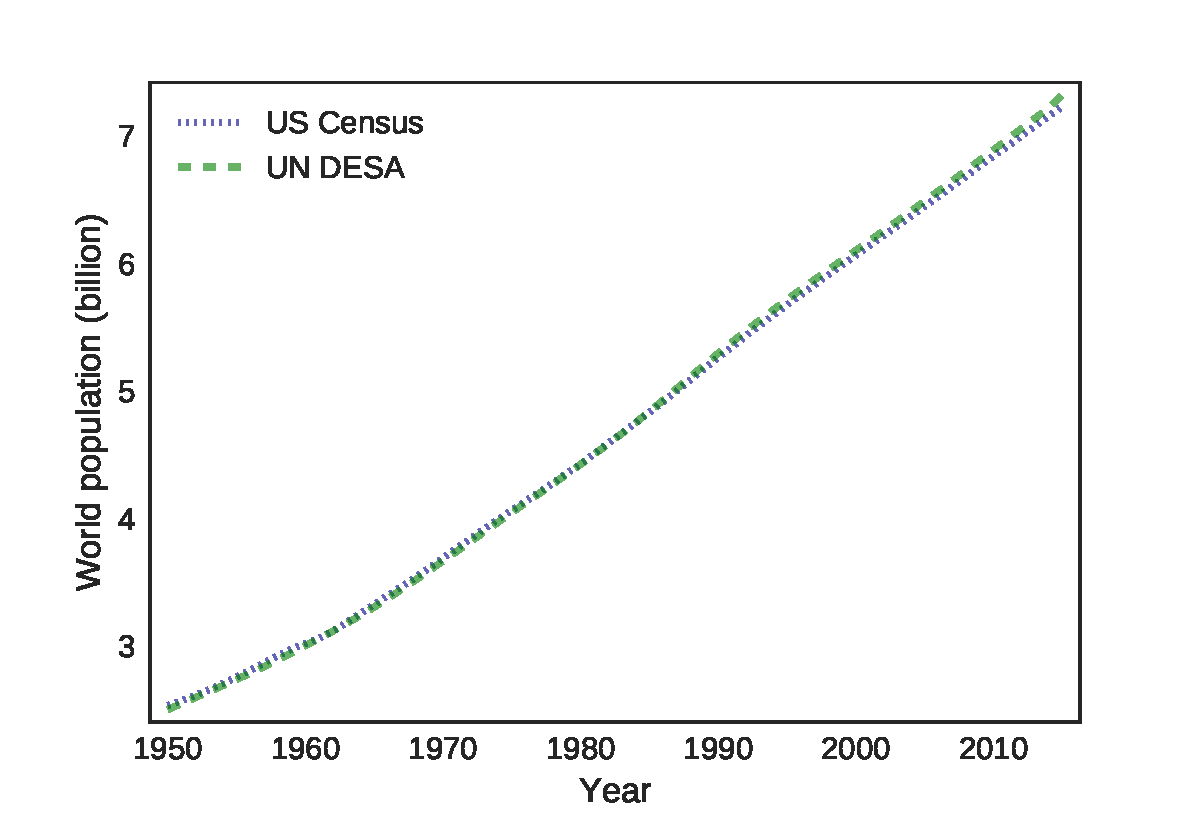
\includegraphics[height=3in]{figs/chap03-fig01.pdf}}
\caption{Estimates of world population, 1950--2015.}
\label{chap03-fig01}
\end{figure}

Figure~\ref{chap03-fig01} shows the result.  Generally the difference between the two estimates is less than 1\%.


\section{Constant growth model}

Suppose we want to predict world population growth over the next 50 or 100 years.  We can do that by developing a model that describes how population grows, fitting the model to the data we have so far, and then using the model to generate predictions.

In the next few sections I will demonstrate this process, starting with simple models, which will turn out not to sufficiently realistic to be credible, and gradually improving them.

Although there is some curvature in the plotted estimates, it looks like world population growth has been close to constant since 1960 or so.  As a starting place, we'll build a model with constant growth.

To fit the model to the data, we'll compute the average annual growth from 1950 to 2015.  Since the UN and Census data are so close, I'll use the Census data, again in terms of billions:

\begin{python}
census = table2.census / 1e9
\end{python}

We can select a value from a \py{Series} using bracket notation:

\begin{python}
census[1950]
\end{python}

So we can get the total growth during the interval like this:

\begin{python}
total_growth = census[2015] - census[1950]
\end{python}

But the values 2015 and 1950 are part of the data, so they should not be part of the program.  Putting values like these in the program is called {\bf hard coding}; it is considered bad practice because if the data changes in the future, we would have to modify the program.  For more about hard coding, see \url{https://en.wikipedia.org/wiki/Hard_coding}.

We can get the first and last year from the index, like this:

\begin{python}
first_year = census.index[0]
last_year = census.index[-1]
\end{python}

In brackets, \py{0} selects the first element from \py{census.index}, and \py{-1} selects the last element.  Now we can compute \py{total_growth} and \py{annual_growth}:

\begin{python}
total_growth = census[last_year] - census[first_year]
elapsed_time = last_year - first_year
annual_growth = total_growth / elapsed_time
\end{python}

The next step is to use this estimate to simulate population growth since 1950.

\section{Simulation}

First, we'll make a new \py{TimeSeries} object:

\begin{python}
model = TimeSeries()
\end{python}

A \py{TimeSeries} object contains {\bf time series}, which is a sequence of times and a corresponding sequence of values (see \url{https://en.wikipedia.org/wiki/Time_series}).  In this example the times are years and the values are populations.  

We can set the first value in the new \py{TimeSeries} by copying the first value from \py{census} (we'll get rid of the hard-coded dates soon):

\begin{python}
model[1950] = census[1950]
\end{python}

Then we can set the rest of the values by simulating annual growth:

\begin{python}
for year in arange(1950, 2015):
    model[year+1] = model[year] + annual_growth
\end{python}

The result from \py{arange} is an array of years from 1951 to 2015 (the second argument, 2016, is not included in the range).  In the model, the population each year is the number of the population during the previous year and \py{annual_growth}.

\begin{figure}
% chap03.ipynb.py
\centerline{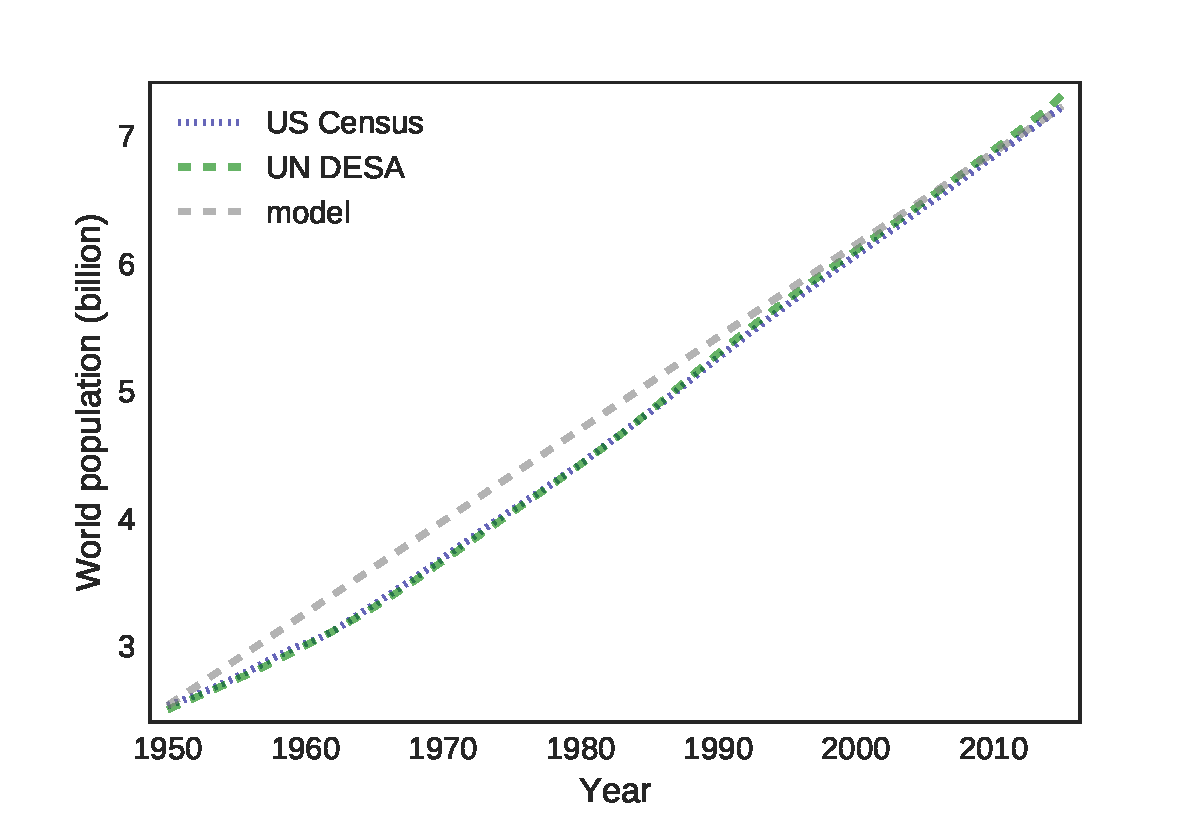
\includegraphics[height=3in]{figs/chap03-fig02.pdf}}
\caption{Estimates of world population, 1950--2015, and a constant growth model.}
\label{chap03-fig02}
\end{figure}

Figure~\ref{chap03-fig02} shows the result. The model does not fit the data particularly well from 1950 to the 1990, but after that, it's pretty good.  Nevertheless, there are problems:

\begin{itemize}

\item There is no plausible mechanism that could cause population growth to be constant from year to year.  Changes in population are determined the fraction of people who die and the fraction of people who give birth, so they should depend on the current population.

\item According to this model, we would expect the population to keep growing at the same rate forever, and that does not seem reasonable.

\end{itemize}

We'll try out some different models in the next few sections, but first let's clean up the code.


\section{Now with system objects}
\label{nowwithsystem}

First, let's put all the information we need to run the model into a \py{System} object:

\begin{python}
system = System(t0=first_year, t_end=last_year,
                p0=census[first_year],
                annual_growth=annual_growth)
\end{python}

\py{t0} and \py{t_end} are the first and last years; \py{p0} is the initial population, and \py{annual_growth} is the estimated annual growth.

Next we'll wrap the code from the previous section in a function:

\begin{python}
def run_simulation1(system):
    model = TimeSeries()
    model[system.t0] = system.p0
    for year in arange(system.t0, system.t_end):
        model[year+1] = model[year] + system.annual_growth
    system.model = model
\end{python}

When \py{run_simulation1} runs, it creates a new series that contains the result of the simulation, and stores it as a new system variable, \py{model}. 

To plot the results, we define a new function:

\begin{python}
def plot_model(system):
    newfig()
    plot_estimates()
    plot(system.model, '--', color='gray', label='model')
    decorate(xlabel='Year', 
             ylabel='World population (billion)',
             ylim=[0, 8])
\end{python}

There's nothing new there except \py{ylim}, which specifies the limits of the $y$ axis, in this case to make the figure look a little better.

Finally, we can run it like this.

\begin{python}
run_simulation1(system)
plot_model(system)
\end{python}

The results are the same as Figure~\ref{chap03-fig02}.

\section{Proportional model}

The biggest problem with the constant growth model is that it doesn't make any sense.    It is hard to imagine how people all over the world could conspire to keep the total constant from year to year.

On the order hand, if some fraction of the population dies each year, and some fraction gives birth, we can compute the net change in the population like this:

\begin{python}
def run_simulation2(system):
    model = TimeSeries()
    model[system.t0] = system.p0
    for year in arange(system.t0, system.t_end):
        births = system.birth_rate * model[year]
        deaths = system.death_rate * model[year]
        model[year+1] = model[year] + births - deaths
    system.model = model
\end{python}

Now we can choose the values of \py{birth_rate} and \py{death_rate} that best fit the data.  Without trying too hard, I chose:

\begin{python}
system.death_rate = 0.01
system.birth_rate = 0.027
\end{python}

Then I ran and plotted the model:

\begin{python}
run_simulation2(system)
plot_model(system)
\end{python}

\begin{figure}
% chap03.ipynb.py
\centerline{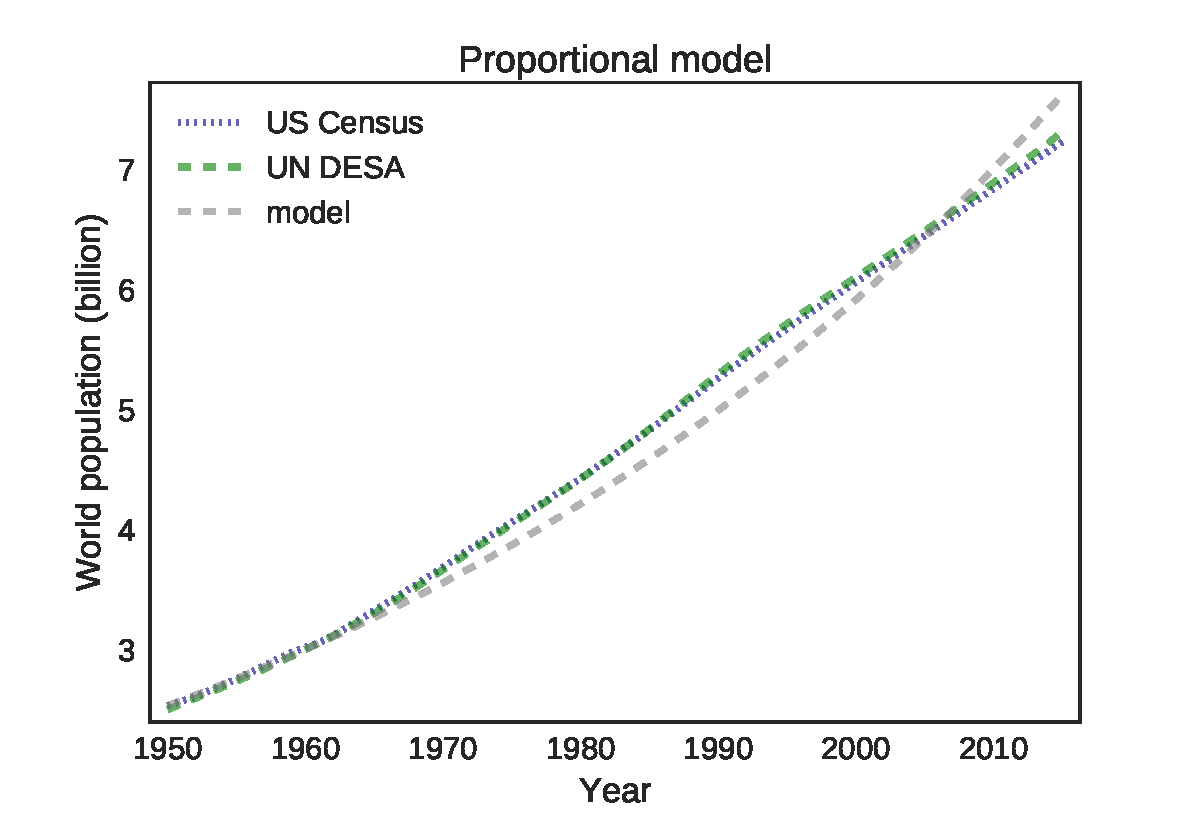
\includegraphics[height=3in]{figs/chap03-fig03.pdf}}
\caption{Estimates of world population, 1950--2015, and a proportional model.}
\label{chap03-fig03}
\end{figure}

Figure~\ref{chap03-fig03} shows the result.  The proportional model fits the data well from 1950 to 1965, but not so well after that.  Overall, the {\bf quality of fit} is not as good as the constant growth model, which is surprising, because it seems like the proportional model is more realistic.

There are a few things we can try to improve the model:

\begin{itemize}

\item Maybe the birth rate and death rate vary over time.

\item Maybe net growth depends on the current population, but the relationship is quadratic, not linear.

\end{itemize}

We will try out these variations, but first, let's clean up the code one more time.

\section{Factoring out the update function}

\py{run_simulation1} and \py{run_simulation2} are nearly identical except for the body of the \py{for} loop, where we compute the population for the next year.

Rather than repeat identical code, we can separate the things that change from the things that don't.  First, we'll pull the body of the loop out and make it a function:

\begin{python}
def update_func1(year, pop, system):
    births = system.birth_rate * pop
    deaths = system.death_rate * pop
    return pop + births - deaths
\end{python}

This function takes as arguments the current year, current population, and a system object, and returns the computed population for the next year.

Now we can write a function that runs any model:

\begin{python}
def run_any_model(system, update_func):
    model = TimeSeries()
    model[system.t0] = system.p0
    for year in arange(system.t0, system.t_end):
        model[year+1] = update_func(year, model[year], system)
    system.model = model
\end{python}

This function demonstrates a feature we have not seen before: it takes a function as a parameter!  When we run \py{run_any_model}, the second parameter is a function, like \py{update_func1}, that computes the population for the next year.

Here's how we call it:

\begin{python}
run_any_model(system, update_func1)
\end{python}

Passing a function as an argument is the same as passing any other value.  The argument, which is \py{update_func1} in this example, gets assigned to the parameter, which is called \py{update_func}.  Inside \py{run_any_model}, we can run \py{update_func} just like any other function.

When you run \py{run_any_model}, it runs \py{update_func1} once for each year between \py{t0} and \py{t_end}.  The result is the same as Figure~\ref{chap03-fig03}.


\section{Combining birth and death}

While we are at it, we can also simplify the code by combining births and deaths to compute the net growth rate.  Instead of two parameters, \py{birth_rate} and \py{death_rate}, we can write the update function in terms of a single parameter that represents the difference

\begin{python}
system.alpha = system.birth_rate - system.death_rate
\end{python}

Here's the modified version of \py{update_func1}:

\begin{python}
def update_func1b(year, pop, system):
    net_growth = system.alpha  * pop
    return pop + net_growth
\end{python}

And here's how we run it:

\begin{python}
run_any_model(system, update_func1b)
\end{python}

Again, the result is the same as Figure~\ref{chap03-fig03}.


\section{Quadratic growth}
\label{quadratic}

It makes sense that net growth should depend on the current population, but maybe it's not a linear relationship, like this:

\begin{python}
    net_growth = system.alpha * pop
\end{python}

Maybe it's a quadratic relationship, like this:

\begin{python}
    net_growth = system.alpha * pop + system.beta * pop**2
\end{python}

We can test that conjecture with a new update function:

\begin{python}
def update_func3(year, pop, system):
    net_growth = system.alpha * pop + system.beta * pop**2
    return pop + net_growth
\end{python}

Now we need two parameters.  I chose these values by trial and error; we will see better ways to do it later.

\begin{python}
system.alpha = 0.025
system.beta = -0.0018
\end{python}

And here's how we run it:

\begin{python}
run_any_model(system, update_func3)
\end{python}

\begin{figure}
% chap03.ipynb.py
\centerline{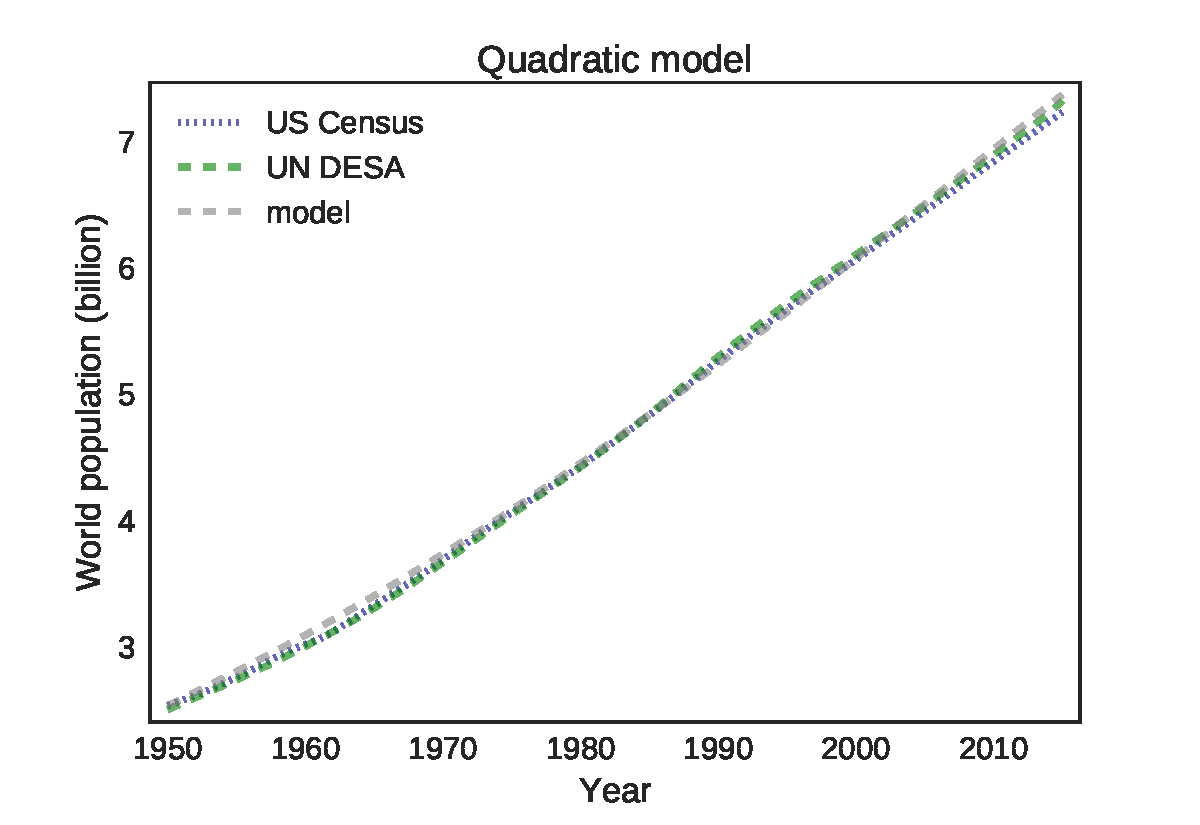
\includegraphics[height=3in]{figs/chap03-fig04.pdf}}
\caption{Estimates of world population, 1950--2015, and a quadratic model.}
\label{chap03-fig04}
\end{figure}

Figure~\ref{chap03-fig04} shows the result.  The model fits the data well over the whole range, with just a bit of daylight between them, in the 1960s.

Of course, we should expect the quadratic model to fit better than the linear or proportional model because it has two parameters we can choose, where the other models have only one.  In general, the more parameters you have to play with, the better you should expect the model to fit.

But fitting the data is not the only reason to think the quadratic model might be a good choice; it also makes sense, that is, there is a legitimate reason to expect the relationship between growth and population to have this form.

To understand it, let's look at net growth as a function of population.  Here's how we compute it:

\begin{python}
pop_array = linspace(0.001, 15, 100)
net_growth_array = (system.alpha * pop_array + 
                    system.beta * pop_array**2)
\end{python}

\py{pop_array} contains 100 equally spaced values from near 0 to 15.  \py{net_growth_array} contains the corresponding 100 values of net growth.  We can plot the results like this: 

\begin{python}
plot(pop_array, net_growth_array, '-')
\end{python}

\begin{figure}
% chap03.ipynb.py
\centerline{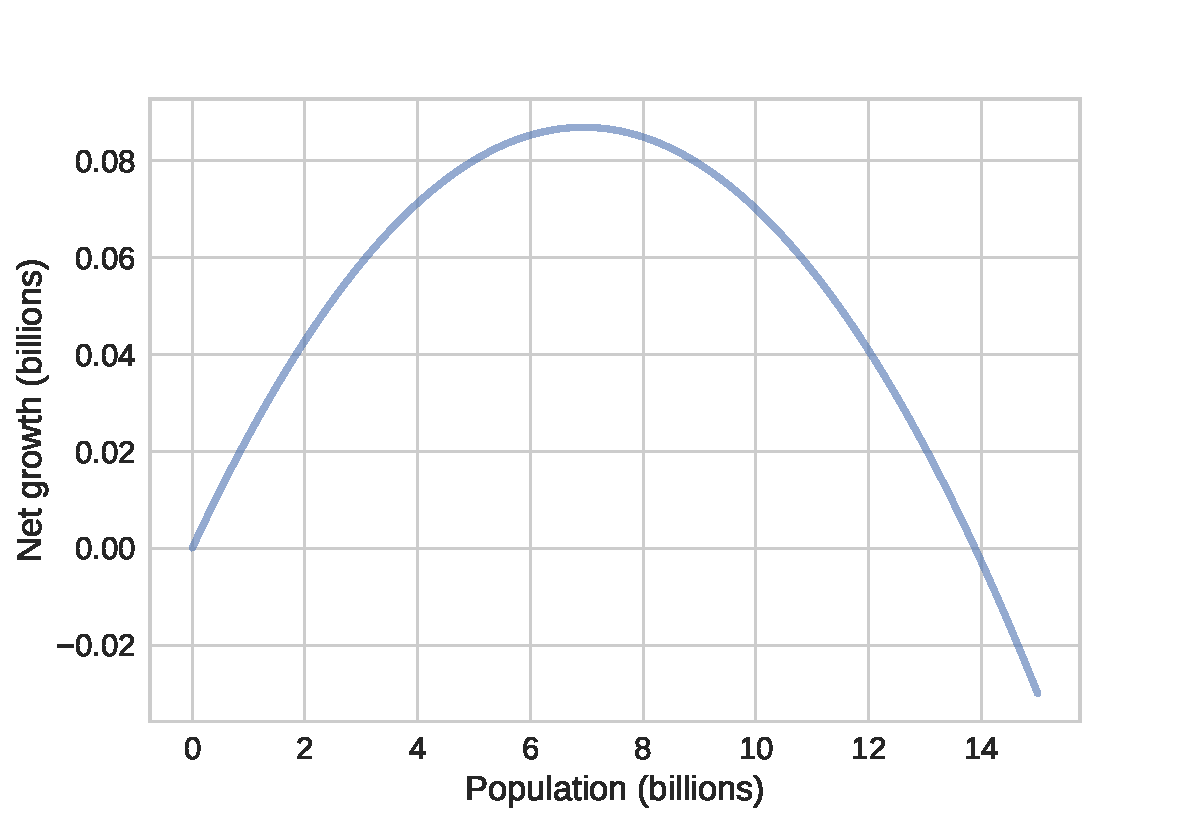
\includegraphics[height=3in]{figs/chap03-fig05.pdf}}
\caption{Net growth as a function of population.}
\label{chap03-fig05}
\end{figure}

Figure~\ref{chap03-fig05} shows the result.  Note that the x axis is not time, as in the previous figures, but population.  We can divide this curve into four regimes of behavior:

\begin{itemize}

\item When the population is less than 3-4 billion, net growth is proportional to population, as in the proportional model.  In this regime,  the population grows slowly because the population is small.

\item Between 4 billion and 10 billion, the population grows quickly because there are a lot of people, and there are enough resources, like food, water, and space, to sustain high birth rates and low death rates.

\item Above 10 billion, population grows more slowly because resource limits start to decrease birth rates, increase death rates, or both.

\item Above 14 billion, resources are so limited that the death rate exceeds the birth rate and net growth becomes negative.

\end{itemize}

Just below 14 billion, there is a population where net growth is 0, which means that the population does not change.  At this point, the birth and death rates are equal, so the population is in {\bf equilibrium}.

\section{Equilibrium}
\label{equilibrium}

To find this equilibrium point, we can find the roots, or zeros, of this equation:
%
\[ \Delta p = \alpha p + \beta p^2 = 0 \]
%
where $\Delta p$ is net growth, $p$ is current population, and $\alpha$ and $\beta$ are the parameters of the model.  We can rewrite the right hand side like this:
%
\[ \Delta p = p (\alpha + \beta p) = 0 \]
%
which is $0$ when $p=0$ or $p=-\alpha/\beta$.  In this example, $\alpha = 0.025$, $\beta = -0.0018$, and $-\alpha/\beta = 13.9$.

In the context of population modeling, the quadratic model is more conventionally written like this:
%
\[ \Delta p = r p (1 - p / K) \]
%
This is the same model; it's just a different way {\bf parameterize} it.  Given $\alpha$ and $\beta$, we can compute $r=\alpha$ and $K=-\alpha/\beta$.

In this version, it is easier to interpret the parameters: $\alpha$ is the maximum growth rate, observed when $p$ is small, and $K$ is the equilibrium point.  $K$ is also called the {\bf carrying capacity}, since it indicates the maximum population the environment can sustain.

In the next chapter we will use the models we have developed to generate predictions.  But first, a few more thoughts about debugging.

\section{Debugging}

Coming soon.



\chapter{Predict}

Intro

\section{Generating projections}

In the previous chapter we developed a model of world population growth from 1950 to 2016.  The is simple, but it fits the data well and the mechanisms it is based on are plausible.  Now we can use it to generate projections.

We'll start with the quadratic model from Section~\ref{quadratic}, which is based on this update function:

\begin{python}
def update_func3(year, pop, system):
    net_growth = system.alpha * pop + system.beta * pop**2
    return pop + net_growth
\end{python}

As we saw in the previous chapter, we can get the start date, end date, and initial population from \py{census}, which is a series that contains world population estimates generated by the U.S. Census:

\begin{python}
t0 = census.index[0]
t_end = census.index[-1]
p0 = census[t0]
\end{python}

Now we can initialize a system object:

\begin{python}
system = System(t0=t0, 
              t_end=t_end,
              p0=p0,
              alpha = 0.025,
              beta = -0.0018)
\end{python}

And run the model:

\begin{python}
run_any_model(system, update_func3)
\end{python}

We have already seen the results in Figure~\ref{chap03-fig04}.


Now, to generate a projection, the only thing we have to change is \py{t_end}:

\begin{python}
system.t_end = 2250
run_any_model(system, update_func3)
\end{python}

\begin{figure}
% chap03.ipynb.py
\centerline{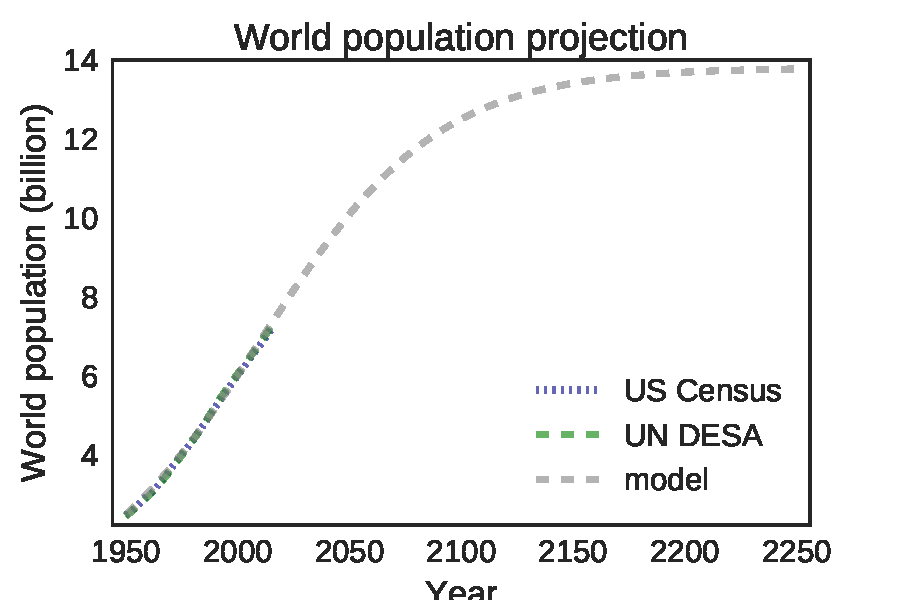
\includegraphics[height=3in]{figs/chap04-fig01.pdf}}
\caption{Quadratic model of world population growth, with projection from 2016 to 2250.}
\label{chap04-fig01}
\end{figure}

Figure~\ref{chap04-fig01} shows the result, with a projection until 2250.  According to this model, population growth will continue almost linearly for the next 50--100 years, then slow over the following 100 years, approaching 13.9 billion by 2250.

I am using the word ``projection" deliberately, rather than ``prediction", with the following distinction: ``prediction" implies something like ``this is what we should reasonably expect to happen, at least approximately"; ``projection" implies something like ``if this model is actually a good description of what is happening in this system, and if nothing in the future causes the parameters of the model to change, this is what would happen."

Using ``projection" leaves open the possibility that there are important things in the real world that are not captured in the model, and even if the model is good, that the parameters might change.

In this example, the model is based on the assumption that population growth is limited by the availability of resources; in that scenario, as the population approaches the carrying capacity, birth rates fall and death rates rise because resources become scarce.

And if that's the case, it might be possible to use actual population growth to estimate carrying capacity, especially if we observe the transition into the regime where the growth rate starts to fall.

But in the case of world population growth, these conditions don't apply:

\begin{itemize}

\item Over the last 50 years, the net growth rate has leveled off, but not yet started to fall, so we don't have enough data to estimate carrying capacity accurately.

\item Resource limitations are probably {\em not} the primary reason the growth rate has slowed. 

\end{itemize} 

First, the death rate is not increasing; rather, it has declined from 1.9\% in 1950 to 0.8\% now (see \url{https://en.wikipedia.org/wiki/Mortality_rate}).

So the decrease in net growth is due entirely to declining birth rates.  And there are many reasons birth rates are falling, but resource limitations are not among them; in fact, it's almost the opposite.  As nations develop and people become more wealthy, birth rates tend to fall.  


\section{Comparing projections}

If recent changes in birth and death rates are not caused by resource limitations, we should not expect the long-term predictions of this model to be accurate.

However, the same agencies and researchers that produce population estimates also produce projections, and we can compare theirs to ours.  Table 3 from \url{https://en.wikipedia.org/wiki/World_population_estimates} contains projections from the U.S. Census and the United Nations DESA:

\begin{python}
table3 = tables[3]
\end{python}

We can plot their projections like this:

\begin{python}
def plot_projections(table):
    census = table.census / 1e9
    un = table.un / 1e9
    
    plot(census, ':', color='darkblue', label='US Census')
    plot(un.dropna(), '--', color='green', label='UN DESA')
\end{python}

When we plot the UN data, we use \py{dropna}; it removes from the \py{Series} any elements that contain the special value \py{NaN}, which indicates missing data (in this case, years where the UN did not produce an estimate).

We can run our model over the same interval:

\begin{python}
system.t_end = 2100
run_any_model(system, update_func3)
\end{python}


\begin{figure}
\centerline{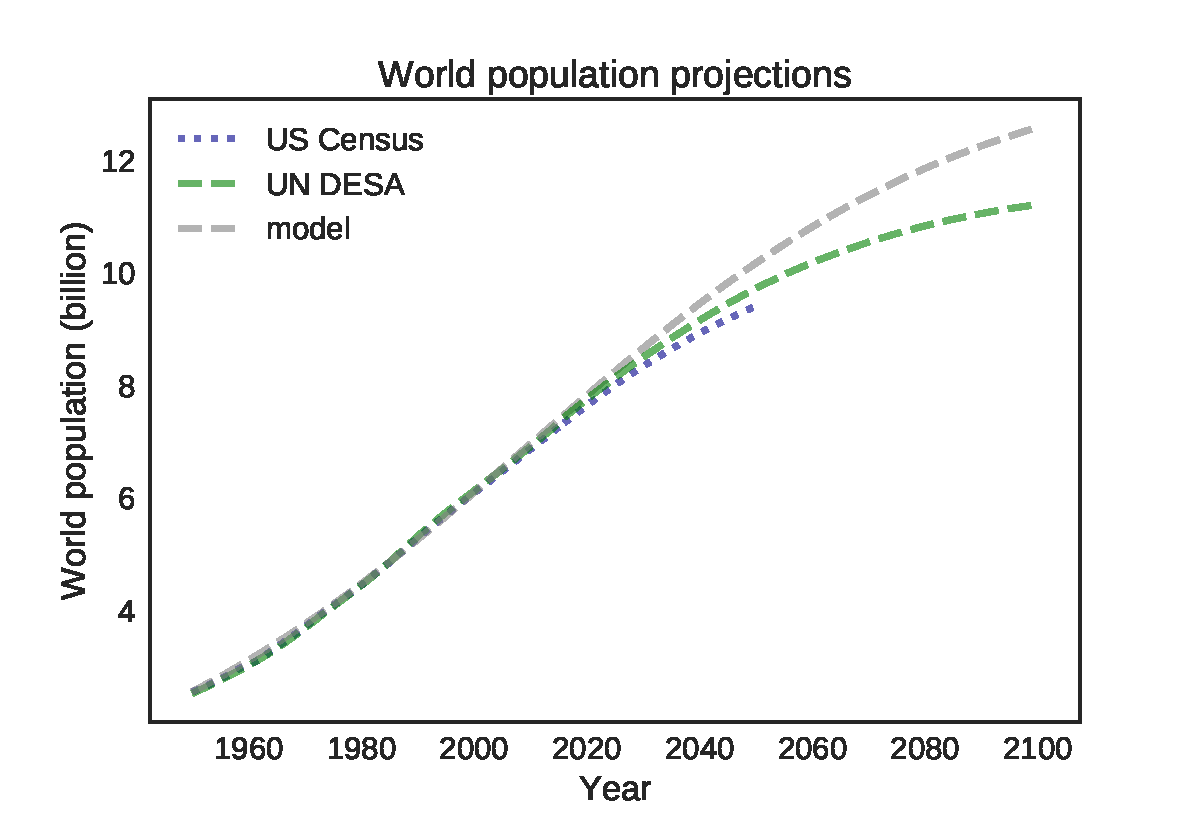
\includegraphics[height=3in]{figs/chap04-fig02.pdf}}
\caption{Projections of world population generated by the U.S. Census Bureau, the United Nations, and our quadratic model.}
\label{chap04-fig02}
\end{figure}

And compare our projections to theirs.  Figure~\ref{chap04-fig02} shows the results.  People who know what they are doing expect world population to grow more slowly than our model projects, probably because their models are broken down by region and country, where conditions are different, and they take into account expected economic development.

Nevertheless, their projections are qualitatively similar to ours, and theirs differ with each other almost as much as they differ with ours.  So the result from this model, simple as it is, are not entirely crazy.


\section{Difference equations}

The population models in the previous chapter and this one are simple enough that we didn't really need to run simulations.  We could have solved them mathematically.  For example, we wrote the constant growth model like this:

\begin{python}
model[year+1] = model[year] + annual_growth
\end{python}

In mathematical notation, we would write the same model like this:
%
\[ x_{n+1} = x_n + c \]
%
where $x_n$ is the population during year $n$, $x_0$ is a given initial population, and $c$ is constant annual growth.  This way of representing the model is a {\bf recurrence relation}; see \url{https://en.wikipedia.org/wiki/Recurrence_relation}.

Often it is possible to solve a recurrence relation by writing an equation that computes $x_n$, for a given value of $n$, directly; that is, without computing the intervening values from $x_1$ through $x_{n-1}$.

In the case of constant growth we can see that $x_1 = x_0 + c$, and $x_2 = x_1 + c$.  Combining these, we get $x_2 = x_0 + 2c$, then $x_3 = x_0 + 3c$, and it is not hard to conclude that in general
%
\[ x_n = x_0 + nc \]
%
So if we want to know $x_100$ and we don't care about the other values, we can compute it with one multiplication and one addition.

We can also write the proportional model as a recurrence relation:
%
\[ x_{n+1} = x_n + \alpha x_n \]
%
Or more conventionally as:
%
\[ x_{n+1} = x_n (1 + \alpha) \]
%
Now we can see that $x_1 = x_0 (1 + \alpha)$, and $x_2 = x_0 (1 + \alpha)^2$, and in general
%
\[ x_n = x_0 (1 + \alpha)^n \]
%
This result is a {\bf geometric progression}; see \url{https://en.wikipedia.org/wiki/Geometric_progression}.  When $\alpha$ is positive, the factor $1+\alpha$ is greater than 1, so the elements of the sequence grow without bound.

Finally, we can write the quadratic model like this:
%
\[ x_{n+1} = x_n + \alpha x_n + \beta x_n^2 \]
%
or with the more conventional parameterization like this:
%
\[ x_{n+1} = x_n + r x_n (1 - x_n / K) \]
%
There is no analytic solution to this equation, but we can approximate it with a differential equation and solve that, which is what we'll do in the next section.


\section{Differential equations}
\label{diffeq}

Starting again with the constant growth model
%
\[ x_{n+1} = x_n + c \]
%
If we define $\Delta x$ to be the change in $x$ from one time step to the next, we can write:
%
\[ \Delta x = x_{n+1} - x_n = c \]
%
If we define $\Delta t$ to be the time step, which is one year in the example, we can write the rate of change per unit of time like this:
%
\[ \frac{\Delta x}{\Delta t} = c \]
%
This model is {\bf discrete}, which means it is only defined at integer values of $n$ and not in between.  But in reality, people are born and die all the time, not once a year, so a {\bf continuous} model might be more realistic.

We can make this model continuous by writing the rate of change in the form of a derivative:
%
\[ \frac{dx}{dt} = c \]
%
This way of representing the model is a {\bf differential equation}; see \url{https://en.wikipedia.org/wiki/Differential_equation}.  We can solve this differential equation by integrating both sides, which yields:
%
\[ x(t) = \int c~dt = c t + x_0 \]
%
Similarly, we can rewrite the proportional growth model like this:
%
\[ \frac{\Delta x}{\Delta t} = \alpha x \]
%
And as a differential equation like this:
%
\[ \frac{dx}{dt} = \alpha x \]
%
If we multiply both sides by $dt$ and divide by $x$, we get
%
\[ \frac{1}{x} dx = \alpha~dt \] 
%
Now we can take the antiderivative of both sides, yielding:
%
\[ \ln x = \alpha t + const \]
%
where $\ln$ is the natural logarithm and $const$ is the constant of integration.  Raising $e$ to both sides, we have
%
\[ x = e^{\alpha t + const} \]
%
which we can rewrite
%
\[ x = e^{\alpha t} e^{const} \]
%
Since $e$ raised to an arbitrary constant is just another arbitrary constant, we can write
%
\[ x = Ce^{\alpha t} \]
%
where $A = e^{const}$.  Or using an alternative notation I prefer:
%
\[ x(t) = C \exp(\alpha t) \]
%
So there are many solutions to this differential equation, with different values of $C$.  The particular solution we want is the one that has the value $x_0$ when $t=0$.  Well, when $t=0$, $x(t) = C$, so $C = x_0$ and the solution we want is

\[ x(t) = x_0 \exp(\alpha t) \]

If you would like to see this derivation done a little more carefully, you might like this video: \url{https://www.khanacademy.org/math/ap-calculus-ab/diff-equations-ab/exponential-models-ab/v/exponential-solution-to-differential-equation}.


\section{Analysis and simulation}

Once you have designed a model, there are generally two ways to proceed: simulation and analysis.  Simulation often comes in the form of a computer program that models changes in a system over time, like births and deaths, or bikes moving from place to place.  Analysis often comes in the form of algebra; that is, symbolic manipulation using mathematical notation.

Analysis and simulation have different capabilities and limitations.  Simulation is generally more versatile; it is easy to add and remove parts of a program and test many versions of a model, as we have done in the previous examples.

But there are several things we can do with analysis that are harder or impossible with simulations:

\begin{itemize}

\item With analysis we can sometimes compute, exactly and efficiently, a value that we could only approximate, less efficiently, with simulation.  For example, in Figure~\ref{chap03-fig05}, we can see that net growth goes to zero near 14 billion, and we could estimate carrying capacity using a numerical search algorithm (more about that later).  But with the analysis in Section~\ref{quadratic}, we get the general result that $K=-\alpha/\beta$.

\item Analysis often provides ``computational shortcuts", that is, the ability to jump forward in time to compute the state of a system many time steps in the future without computing the intervening states.

\item We can use analysis to state and prove generalizations about models; for example, we might prove that certain results will always or never occur.  With simulations, we can show examples and sometimes find counterexamples, but it is hard to write proofs.

\item And analysis can provide insight into models and the systems they describe; for example, sometimes we can identify regimes of qualitatively different behavior and key parameters that control those behaviors.

\end{itemize}

When people see what analysis can do, they sometimes get drunk with power, and imagine that it gives them a special ability to see past the veil of the material world and glimpse the laws of mathematics that govern the universe.  When they analyze a model of a physical system, they talk about ``the math behind it" as if our world is the mere shadow of a world of ideal mathematical entities\footnote{I am not making this up; see \url{https://en.wikipedia.org/wiki/Allegory_of_the_Cave}.}.

This is, of course, nonsense.  Mathematical notation is a language designed by humans for a purpose, specifically to facilitate symbolic manipulations like algebra.  Similarly, programming languages are designed  for a purpose, specifically to represent computational ideas and run programs.

Each of these languages is good for the purposes it was designed for and less good for other purposes.  But they are often complementary, and one of the goals of this book is to show how they can be used together.


\section{Analysis with WolframAlpha}

Traditionally most analysis was done by dragging sticks of graphite across wood pulp, a process that is laborious an error-prone.  A useful alternative is symbolic computation.  If you have used services like WolframAlpha, you have used symbolic computation.

For example, if you go to \url{https://www.wolframalpha.com/} and type

\begin{python}
df(t) / dt = alpha f(t)
\end{python}

WolframAlpha infers that $f(t)$ is a function of $t$ and $alpha$ is a parameter, it classifies the query as a ``first-order linear ordinary differential equation", and reports the general solution:
%
\[ f(t) = c_1 e^{\alpha t} \]
%
If you add a second equation to specify the initial condition:

\begin{python}
df(t) / dt = alpha f(t),  f(0) = p0
\end{python}

WolframAlpha reports the particular solution:

\[ f(t) = p0 e^{\alpha t} \]

WolframAlpha is based on Mathematica, a powerful programming language designed specifically for symbolic computation.


\section{Analysis with SymPy}

Python has a module called SymPy that provides symbolic computation tools similar to Mathematica.  They are not as easy to use as WolframAlpha, but they have some other advantages.

First, we have to import the tools we plan to use:

\begin{python}
from sympy import symbols, Function, diff, dsolve
\end{python}

Because SymPy is integrated into Python, we have to distinguish between normal Python variables and SymPy symbols.  \py{symbols} takes a string and returns a symbol object.  So if we run this assignment:

\begin{python}
t = symbols('t')
\end{python}

Python understands that \py{t} should be treated as a symbol, rather than a number.  If we now run

\begin{python}
expr = t + 1
\end{python}

Python doesn't try to perform addition; rather, it creates a new symbol object that represents the sum of \py{t} and \py{1}.  Later we can evaluate this sum using \py{subs}, which substitutes a value for a symbol.  This example substitutes 2 for \py{t}:

\begin{python}
expr.subs(t, 2)
\end{python}

The result is 3.

Functions in SymPy are represented by a special class of symbol:

\begin{python}
f = symbols('f', cls=Function)
\end{python}

Now if we write \py{f(t)}, we get an object that represents the evaluation of a function, $f$, at a value, $t$.  But again it doesn't actually try to evaluate it.

\section{Differential equations in SymPy}

SymPy provides a function, \py{diff}, that performs differentiation.  We can apply it to \py{f(t)} like this:

\begin{python}
dfdt = diff(f(t), t)
\end{python}

The result is (you guessed it) an object that represents the derivative of \py{f} with respect to \py{t}.  But again, it doesn't try to compute the derivative yet.

To represent a differential equation, we use \py{Eq}:

\begin{python}
alpha = symbols('alpha')
eq1 = Eq(dfdt, alpha*f(t))
\end{python}

The result is an object that represents an equation, which is displayed like this:
%
\[ \frac{d}{d t} f{\left (t \right )} = \alpha f{\left (t \right )} \]
%
Now we can use \py{dsolve} to solve this differential equation:

\begin{python}
solution_eq = dsolve(eq1)
\end{python}

The result is the equation
%
\[ f{\left (t \right )} = C_{1} e^{\alpha t} \]
%
which should look familiar.  This is the general solution, which still contains an unspecified constant, $C_1$.  

To get the particular solution where $f(0) = p_0$, we substitute \py{p0} for \py{C1}.  First, we have to create two more symbols:

\begin{python}
C1, p0 = symbols(['C1', 'p0'])
\end{python}

Now we can perform the substitution:

\begin{python}
particular = solution_eq.subs(C1, p0)
\end{python}

The result is 
%
\[ f{\left (t \right )} = p_{0} e^{\alpha t} \]
%
This function is called the {\bf exponential growth curve}; see \url{https://en.wikipedia.org/wiki/Exponential_growth}.


\section{Solving the quadratic growth model}

In the notebook for this chapter, you will see how to use the same tools to solve the quadratic growth model with parameters $r$ and $K$.  The general solution is
%
\[ f{\left (t \right )} = \frac{K e^{C_{1} K + r t}}{e^{C_{1} K + r t} - 1} \]
%
To get the particular solution where $f(0) = p_0$, we evaluate the general solution at $t=0$, which yields:
%
\[ f(0) = \frac{K e^{C_{1} K}}{e^{C_{1} K} - 1} \]
%
Then we set this expression equal to $p_0$ and solve for $C_1$.  The result is:
%
\[ C_1 = \frac{1}{K} \log{\left (- \frac{p_{0}}{K - p_{0}} \right )} \]
%
Finally, we substitute this value of $C_1$ into the general solution, which yields:
%
\[ f(t) = \frac{K p_{0} e^{r t}}{K + p_{0} e^{r t} - p_{0}} \]
%
This function is called the {\bf logistic growth curve}; see \url{https://en.wikipedia.org/wiki/Logistic_function}.  In the context of growth models, the logistic function is often written
%
\[ f(t) = \frac{K}{1 + A e^{-rt}} \]
%
where $A = (K - p_0) / p_0$.  In the notebook, you'll see how to use SymPy to confirm that the two ways to write the solution are equivalent.

If you would like to see this differential equation solved by hand, you might like this video: \url{https://www.khanacademy.org/math/ap-calculus-bc/diff-equations-bc/logistic-diff-eq-bc/v/solving-logistic-differential-equation-part-1}


\section{Summary}

The following table summarizes the results so far:

\begin{tabular}{l|l|l} 
         & Discrete & Continuous \\ 
\hline 
Constant & linear: $x_n = p_0 + \alpha n$ & linear: $x(t) = p_0 + \alpha t$ \\ 
 
Proportional & geometric: $x_n = p_0(1+\alpha)^n$ & exponential: $x(t) = p_0 \exp(\alpha t)$ \\ 
 
Quadratic &  & logistic: $x(t) = \frac{K p_0 \exp(rt)}{K + \exp(rt) - p_0}$ \\ 
\end{tabular} 

What we've been calling the constant growth model is more commonly called ``linear growth" because the solution is a line.  Similarly, what's we've called proportion is commonly called ``exponential growth", and what we've called quadratic is commonly called ``logistic".

I avoided the more common terms because I thought it would seem strange to use them before we solved the equations and discovered the functional form of the solutions.




\chapter{Design}

Intro

My presentation of the SIR model in this chapter, and the analysis in the next chapter, is based on an excellent article by David Smith and Lang Moore\footnote{Smith and Moore, ``The SIR Model for Spread of Disease," Journal of Online Mathematics and its Applications, December 2001, at \url{https://www.maa.org/press/periodicals/loci/joma/the-sir-model-for-spread-of-disease}.}.

\section{The Freshman Plague}

Every year at Olin College, about 90 new students come to campus from around the country and the world.  Most of them arrive healthy and happy, but we should expect at least one, by chance, to come with some kind of infectious disease.  A few weeks later, predictably, some fraction of the incoming class comes down with what we call ``The Freshman Plague".

In this chapter we introduce a well-known model of infectious disease, the Kermack-McKendrick model, and use it to explain the progression of the disease over the course of the semester, predict the effect of possible interventions (like immunization) and design the most effective intervention campaign.

Normally we like to do our own modeling; that is, we start with a physical system, identify factors that seem likely to be important, and think about how to represent them in a model.  In this chapter we start with an existing model and reverse-engineer it.  Along the way, we will think about the modeling decisions that went into it and identify its capabilities and limitations.

\section{The SIR model}

The Kermack-McKendrick model is a simple version of an ``SIR model", so-named because it considers three categories of people:

\begin{itemize}

\item {\bf S}: People who are ``susceptible", that is, capable of contracting the disease if they come into contact with someone who is infected.

\item {\bf I}: People who are ``infected" or, more specifically, capable of passing along the disease if they come into contact with someone susceptible.

\item {\bf R}: People who have ``recovered".

\end{itemize}
  
In the basic version of the model, people who have recovered are considered to be immune to reinfection.  That is a reasonable model for some diseases, but not for others, so it should be on the list of assumptions to reconsider later.

Let's think about how we should expect the number of people in each of these categories to change over time.  Suppose we know that people with the disease are infectious for a period of 4 days, on average.  If 100 people are infectious at a particular point in time, and we ignore the particular time each one became infected, we expect about 1 out of 4 to recover on any particular day.

Putting that a different way, if the time between recoveries is 4 days, the recovery rate is about 0.25 recoveries per day, which we'll denote with the parameter $\gamma$ (the Greek letter gamma).  If the total number of people in the population is $N$, and the fraction currently infected is $i$, the total number of recoveries we expect per day is $\gamma i N$.

Now let's think about the number of new infections.  Suppose we know that each susceptible person comes into contact with 1 person every 3 days, on average, in such a way that they would contract the disease if the other person is infected.  We'll denote this contact rate with the parameter $\beta$ (the Greek letter beta).

It's probably not reasonable to assume that we know $\beta$ ahead of time, but later we'll see how we could estimate it based on data from previous semesters.

If $s$ is the fraction of the population that's susceptible, $s N$ is the number of susceptible people, $\beta s N$ is the number of contacts per day, and $\beta s i N$ is the number of those contacts where the other person is infectious.

In summary:

\begin{itemize}

\item The number of recoveries we expect per day is $\gamma i N$; dividing by $N$ yields the fraction of the population that recovers in a day, which is $\gamma i$.

\item The number of new infections we expect per day is $\beta s i N$; dividing by $N$ yields the fraction of the population that gets infected in a day, which is $\beta s i$.

\end{itemize}

This model assumes that the population is closed, that is, no one arrives or departs.  So the size of the population, $N$, is constant.


\section{The SIR equations}
\label{sireqn}

If we treat time as a continuous quantity, we can write differential equations that describe the rates of change for $s$, $i$, and $r$ (where $r$ is the fraction of the population that has recovered):
%
\begin{align*}
\frac{ds}{dt} &= -\beta s i \\
\frac{di}{dt} &= \beta s i - \gamma i\\
\frac{dr}{dt} &= \gamma i
\end{align*}
%
To avoid cluttering the equations, I leave it implied that $s$ is a function of time, $s(t)$, and likewise for $i$ and $r$.

SIR models are examples of {\bf compartment models}, so-called because they divide the world into discrete categories, or compartments, and describe transitions from one compartment to another.  Compartments are also called {\bf stocks} and transitions between them are called {\bf flows}.

In this example, there are three stocks --- susceptible, infected, and recovered --- and two flows --- new infections and recoveries.  Compartment models are often represented visually using stock-and-flow diagrams (see \url{https://en.wikipedia.org/wiki/Stock_and_flow}.

\begin{figure}
%http://yuml.me/edit/3de9c163
\centerline{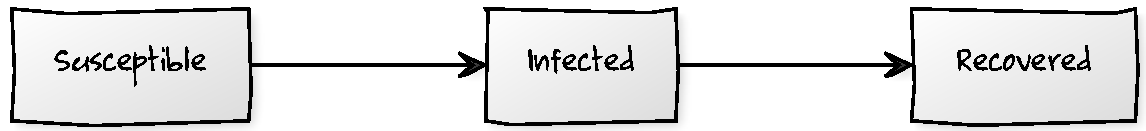
\includegraphics[width=4.5in]{figs/stock_flow1.pdf}}
\caption{Stock and flow diagram for an SIR model.}
\label{stock_flow1}
\end{figure}

Figure~\ref{stock_flow1} shows the stock and flow diagram for an SIR model.



\section{Implementation}

For a given physical system, there are many possible models, and for a given model, there are many ways to represent it.  For example, we can represent an SIR model as a stock-and-flow diagram, as a set of differential equations, or as a Python program.

The process of representing a model in these forms is called {\bf implementation}.  In this section, we implement the SIR model in Python.

As a first step, I'll represent the initial state of the system using a \py{State} object, which represents a {\bf state vector}, which is a collection of {\bf state variables}.  Each state variable represents information about the system that changes over time (see \url{https://en.wikipedia.org/wiki/State-space_representation}).  

In this example, there are three state variables that represent the fraction of the population in each compartment, \py{S}, \py{I}, and \py{R}.

Creating a \py{State} object is similar to creating a \py{System} object.  We can initialize the \py{State} object with the {\em number} of people in each compartment:

\begin{python}
init = State(S=89, I=1, R=0)
\end{python}

And the convert the numbers to fractions by dividing through by the total:

\begin{python}
init /= np.sum(init)
\end{python}

For now, let's assume we know the time between contacts and time between recoveries:

\begin{python}
tc = 3             # time between contacts in days 
tr = 4             # recovery time in days
\end{python}

In that case we can compute the parameters of the model:

\begin{python}
beta = 1 / tc      # contact rate in per day
gamma = 1 / tr     # recovery rate in per day
\end{python}

Now we need a \py{System} object to store the parameters and initial conditions:

\begin{python}
def make_system(beta, gamma):
    init = State(S=89, I=1, R=0)
    init /= np.sum(init)

    t0 = 0
    t_end = 7 * 14

    return System(init=init, t0=t0, t_end=t_end,
                  beta=beta, gamma=gamma)
\end{python}

This function takes the model parameters as function parameters and returns a new \py{System} object.  The default value for \py{t_end} is 14 weeks, about the length of a semester.


\section{The update function}

At any point in time, the state of the system is represented by a \py{State} object with three values, \py{S}, \py{I} and \py{R}.  The update function takes this series as a parameter, along with the \py{System} object that contains the parameters, and computes the state of the system during the next time step:

\begin{python}
def update1(system, state):
    s, i, r = state

    infected = system.beta * i * s    
    recovered = system.gamma * i
    
    s -= infected
    i += infected - recovered
    r += recovered
    
    return State(S=s, I=i, R=r)
\end{python}

The first line uses a feature we have not seen before, {\bf multiple assignment}.  The value on the right side is a \py{State} that contains three values.  The left hand side is a sequence of three variable names.  The assignment does just what you would want: it assigns the three values from the \py{State} to the three variables, in order.

The update function computes \py{infected} and \py{recovered} as a fraction of the population, then updates \py{s}, \py{i} and \py{r}.  The return value is a \py{State} that contains the updated values.

When we call \py{update1} like this:

\begin{python}
state = update1(sir, init)
\end{python}

The result is the \py{State}

\begin{result}
S    0.985388
I    0.011865
R    0.002747
\end{result}

%TODO: figure out when to talk about integers and floats
%\py{dtype} indicates the type of the data in the \py{State}; \py{float64} %indicates that it contains 64-bit floating-point numbers.  A {\bf %floating-point number} can represent a number with a decimal or %fractional part, as opposed to an integer.


\section{Running the model}

Now we can run the model over a sequence of time steps:

\begin{python}
def run_simulation(system, update_func):
    state = system.init
    for i in arange(system.t0, system.t_end):
        state = update_func(system, state)
    return state
\end{python}

The parameters of \py{run_simulation} are the \py{System} object, which contains the model parameters, initial conditions, and values of \py{t0} and \py{t_end}, and the update function.  The outline of this function should look familiar; it is similar to the function we used for the population model in Section~\ref{nowwithstate}.

We can call \py{run_simulation} like this:

\begin{python}
run_simulation(sir, update1)
\end{python}

The result is the final state of the system:

\begin{result}
S    0.520819
I    0.000676
R    0.478505
\end{result}

This result indicates that after 14 weeks (98 days), about 52\% of the population is still susceptible, which means they were never infected, less than 1\% are actively infected, and 48\% have recovered, which means they were infected at some point.


\section{Collecting the results}

The previous version of \py{run_simulation} only returns the state of the system at the end of the simulation, \py{t_end}, but we might want to see how the state changes over time.  We'll consider two ways to do that: first, using three \py{TimeSeries} objects, then using one \py{DataFrame}.

Here's the first version:

\begin{python}
def run_simulation(system, update_func):
    S = TimeSeries()
    I = TimeSeries()
    R = TimeSeries()

    state = system.init
    t0 = system.t0
    S[t0], I[t0], R[t0] = state
    
    for i in arange(system.t0, system.t_end):
        state = update_func(system, state)
        S[i+1], I[i+1], R[i+1] = state
    
    system.S = S
    system.I = I
    system.R = R
\end{python}

First, we create \py{TimeSeries} objects that will store the results.  

The initial value of \py{state} is a copy of \py{system.init}, which is the \py{State} that contains the initial values of \py{S}, \py{I} and \py{R}.  

Inside the loop, we use \py{update_func} to compute the state of the next time step, then use multiple assignment to unpack the three elements of \py{state} and assign each to the corresponding \py{TimeSeries}.

At the end of the function, we store \py{S}, \py{I}, and \py{R} as attributes of the \py{System} object.

Now we can run the function like this:

\begin{python}
run_simulation(sir, update1)
\end{python}

We'll use the following function to plot the results:

\begin{python}
def plot_results(S, I, R):
    plot(S, '--', color='blue', label='Susceptible')
    plot(I, '-', color='red', label='Infected')
    plot(R, ':', color='green', label='Resistant')
    decorate(xlabel='Time (days)',
             ylabel='Fraction of population')
\end{python}

And run it like this:

\begin{python}
plot_results(sir.S, sir.I, sir.R)
\end{python}

\begin{figure}
\centerline{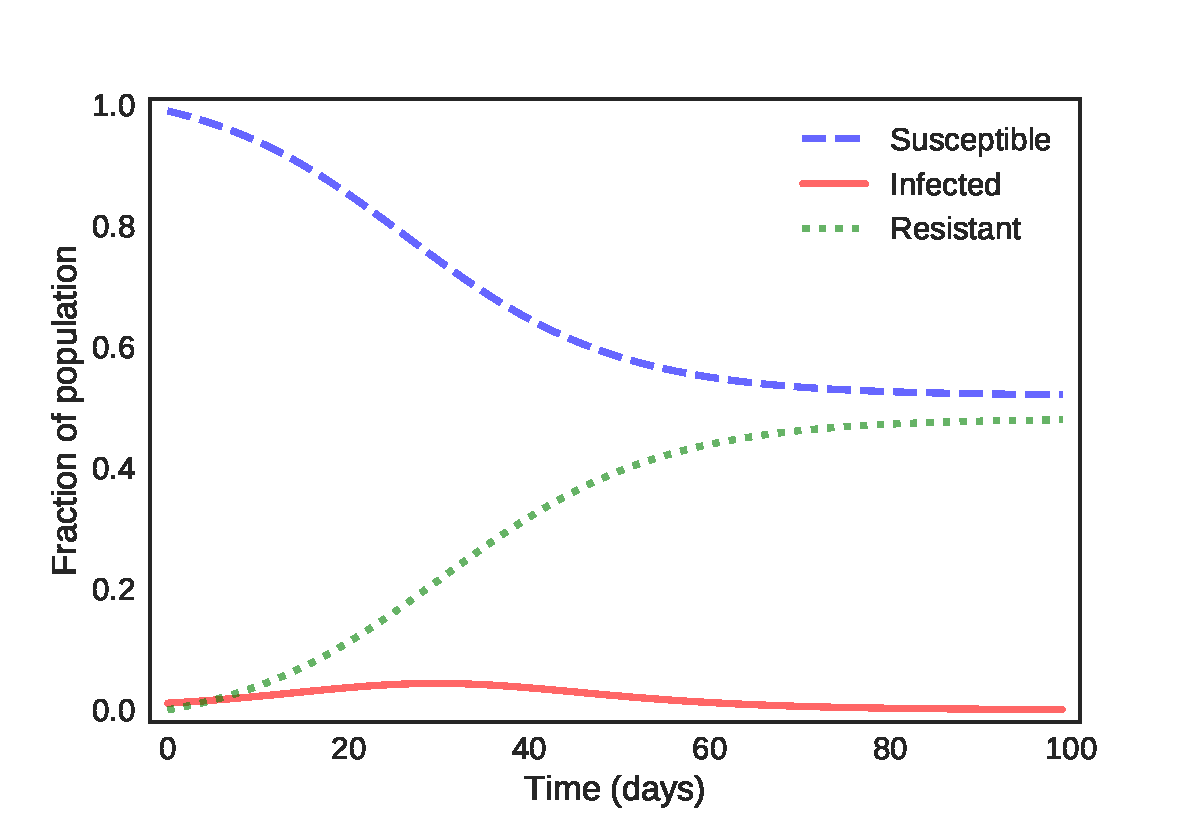
\includegraphics[height=3in]{figs/chap05-fig01.pdf}}
\caption{Time series for \py{S}, \py{I}, and \py{R} over the course of 98 days.}
\label{chap05-fig01}
\end{figure}

Figure~\ref{chap05-fig01} shows the result.  Notice that it takes about three weeks (21 days) for the outbreak to get going, and about six weeks (42 days) before it peaks.  The fraction of the population that's infected is never very high, but it adds up.  In total, almost half the population gets sick. 


\section{Now with a TimeFrame}
\label{timeframe}

If the number of state variables is small, storing them as separate \py{TimeSeries} objects might not be so bad.  But a better alternative is to use a \py{TimeFrame}.  

\py{TimeFrame} objects are defined in \py{modsim.py}.  They are almost identical to the \py{DataFrame} objects we used in Section~\ref{worldpopdata}, with just a few changes I made to make them easier to use for our purposes.  If you want to know the details, you can read about it in \py{modsim.py}.

Here's a more concise version of \py{run_simulation}:

\begin{python}
def run_simulation(system, update_func):
    df = TimeFrame(columns=system.init.index)
    df.loc[system.t0] = system.init
    
    for i in arange(system.t0, system.t_end):
        df.loc[i+1] = update_func(system, df.loc[i])
    
    system.results = df
\end{python}

The first line creates an empty \py{TimeFrame} with one column for each state variables.

Before the loop starts, we want to store the initial conditions in the \py{TimeFrame} at \py{t0}.  Based on the way we've been using \py{TimeSeries} objects, it might be tempting to write:

\begin{python}
df[system.t0] = system.init
\end{python}

The problem is that when you use the bracket operator with a \py{TimeFrame}, it selects a column, not a row.  For example, to select the first column, we could write

\begin{python}
df['S']
\end{python}

The result would be a time series.  To read or write a single row, we have to use \py{loc}, which stands for ``location".  So \py{df.loc[0]} reads a row from a \py{TimeFrame} and 

\begin{python}
df.loc[system.t0] = system.init
\end{python}

assigns the values from \py{system.init} to the first row of \py{df}.  Since the value on the right-hand side is a \py{State}, the assignment matches up the index from the \py{State} with the columns of the \py{TimeFrame}; it assigns the \py{S} value from \py{system.init} to the \py{S} column of the \py{TimeFrame}, and likewise with \py{I} and \py{R}.

We can use the same feature to write the loop more concisely, assigning the \py{State} we get from \py{update_func} directly to the next row of \py{df}.  

Finally, we store \py{df} as a new attribute of \py{system}.  We can call this version of \py{run_simulation} like this:

\begin{python}
run_simulation(sir, update1)
\end{python}

And plot the results like this:

\begin{python}
df = sir.results
plot_results(df.S, df.I, df.R)
\end{python}

As we saw in Section~\ref{series}, we can use dot notation to select columns from the \py{TimeFrame}.


\section{Metrics}

When we plot a time series, we get a view of everything that happened when the model ran, but often we want to boil it down to a few numbers, ideally one, that summarize the outcome.  These summary statistics are called {\bf metrics}.

In the SIR model, we might want to know the time until the peak of the outbreak, the number of people who are sick at the peak, the number of students who will still be sick at the end of the semester, or the total number of students who will be sick at any point.

As an example I will focus on the last one --- the total number of sick students --- and we will consider interventions intended to minimize it.

When a person gets infected, they move from \py{S} to \py{I}, so we can compute the total number of infections like this:

\begin{python}
def calc_total_infected(system):
    df = system.results
    return df.S[system.t0] - df.S[system.t_end]
\end{python}

In the notebook that accompanies this chapter, you will have a chance to write functions that compute other metrics.


\section{Immunization}

Models like this are useful for testing ``what if?" scenarios.  As an example, we'll consider the effect of immunization.

Suppose there is a vaccine that causes a patient to become immune to the Freshman Plague without being infected.  How might you modify the model to capture this effect?

One option is to treat immunization as a short cut from \py{S} to \py{R}, that is, from susceptible to removed (or resistant).  We can implement this feature like this:

\begin{python}
def add_immunization(system, fraction):
    system.init.S -= fraction
    system.init.R += fraction
\end{python}

\py{add_immunization} moves the given fraction of the population from \py{S} to \py{R}.  If we assume that 10\% of students are vaccinated at the beginning of the semester, and the vaccine is 100\% effective, we can simulate the effect like this:

\begin{python}
sir2 = make_system(beta, gamma)
add_immunization(sir2, 0.1)
run_simulation(sir2, update1)
\end{python}

For comparison, we ran the same model without immunization and plot the results.

\begin{figure}
\centerline{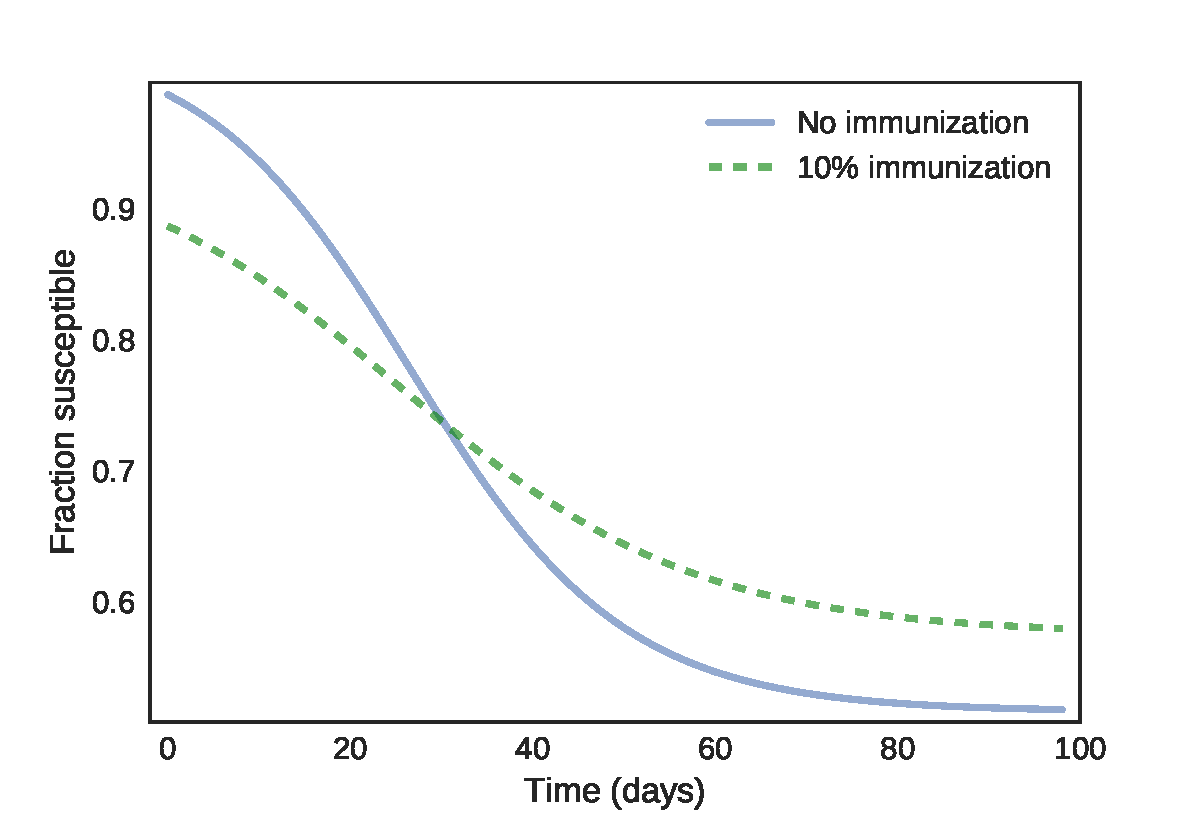
\includegraphics[height=3in]{figs/chap05-fig02.pdf}}
\caption{Time series for \py{S}, with and without immunization.}
\label{chap05-fig02}
\end{figure}

Figure~\ref{chap05-fig02} shows the results, plotting \py{S} as a function of time, with and without immunization.  

Without immunization, almost 47\% of the population is infected at some point.  With 10\% immunization, only 31\% are infected.  That's pretty good.

So let's see what happens if we administer more vaccines.  This function sweeps a range of immunization rates:

\begin{python}
def sweep_immunity(immunize_array):
    sweep = Sweep()
    for fraction in immunize_array:
        sir = make_system(beta, gamma)
        add_immunization(sir, fraction)
        run_simulation(sir, update1)
        sweep[fraction] = calc_total_infected(sir)
    return sweep
\end{python}

The result is a \py{Sweep} object, which is similar to a \py{TimeSeries}; the difference is that the index of the \py{Sweep} contains parameter values, not times.  

Figure~\ref{chap05-fig03} shows a plot of the \py{Sweep}.  Again, notice that the x-axis is the immunization rate, not time.

As the immunization rate increases, the number of infections drops steeply.  If 40\% of the students are immunized, fewer than 4\% get sick.  That's because immunization has two effects: if protects the people who get immunized, of course, but it also protects the rest of the population. 

\begin{figure}
\centerline{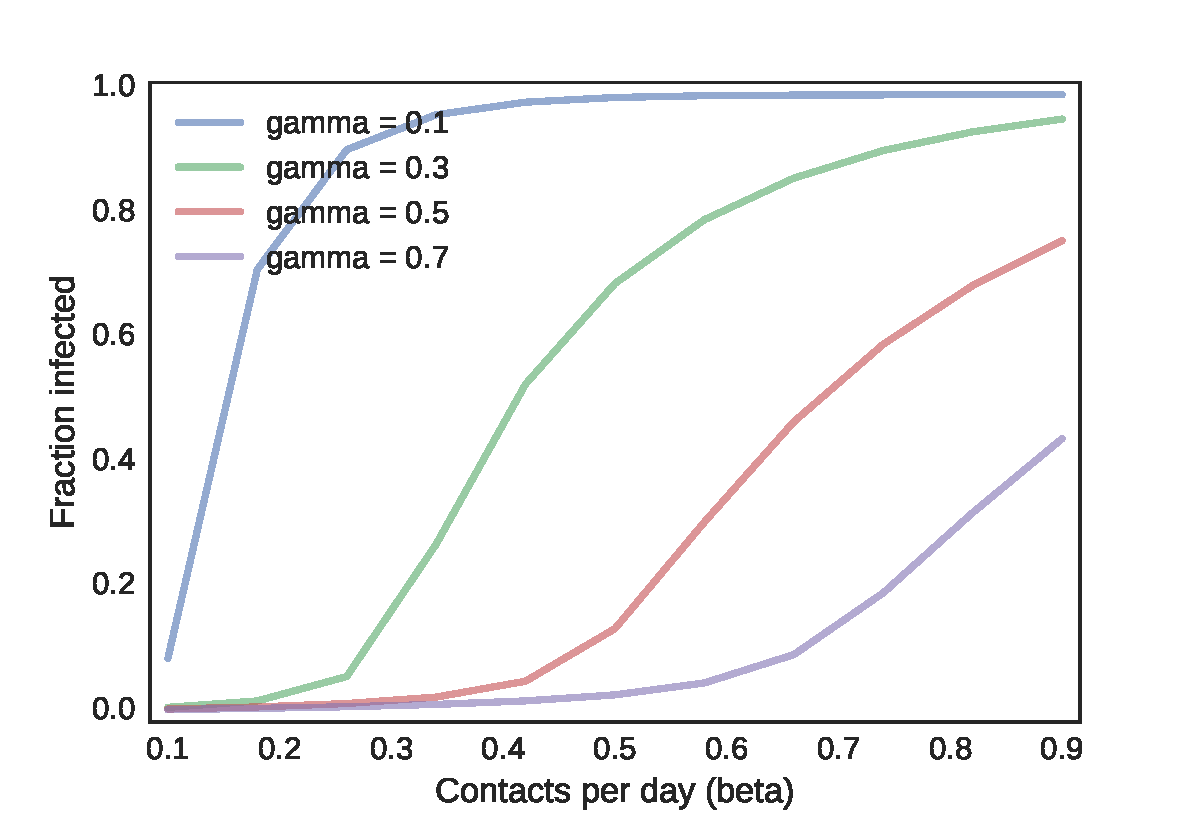
\includegraphics[height=3in]{figs/chap05-fig03.pdf}}
\caption{Fraction of the population infected as a function of immunization rate.}
\label{chap05-fig03}
\end{figure} 

Reducing the number of ``susceptibles" and increasing the number of ``resistants" makes it harder for the disease to spread, because some fraction of contacts are wasted on people who cannot be infected.

This phenomenon is called {\bf herd immunity}, and it is an important element of public health (see \url{https://en.wikipedia.org/wiki/Herd_immunity}).

The steepness of the curve in Figure~\ref{chap05-fig03} is a blessing and a curse.  It's a blessing because it means we don't have to immunize everyone, and vaccines can protect the ``herd" even if they are not 100\% effective.

But it's a curse because a small decrease in immunization can cause a big increase in infections.  In this example, if we drop from 80\% immunization to 60\%, that might not be too bad.  But if we drop from 40\% to 20\%, that would trigger a major outbreak, affecting more than 15\% of the population.  For a serious disease like measles, just to name one, that would be a public health catastrophe.

One use of models like this is to demonstrate phenomena like herd immunity and to predict the effect of interventions like vaccination.  Another use for models is to evaluate alternatives and guide decision making.  We'll see an example in the next section.


\section{Hand washing}

Suppose you are the Dean of Student Affairs, and you have a budget of just \$1200 to try to combat the Freshman Plague.  You have two options for spending this money:

\begin{enumerate}

\item You can pay for vaccinations, at a rate of \$100 per dose.

\item You can spend money on a campaign to remind students to wash hands frequently.

\end{enumerate}

We have already seen how we can model the effect of vaccination.  Now let's think about the hand-washing campaign.  We'll have to answer two questions:

\begin{enumerate}

\item How should we incorporate the effect of hand washing in the model?

\item How should we quantify the effect of the money we spend on a hand-washing campaign?

\end{enumerate}

For the sake of simplicity, let's assume that we have data from a similar campaign at another school, showing that a well-funded campaign can change student behavior enough to reduce the infection rate by 20\%.  

In terms of the model, hand washing has the effect of reducing \py{beta}.  That's not the only way we could incorporate the effect, but it seems reasonable and it's easy to implement.

Now we have to model the relationship between the money we spend and the effectiveness of the campaign.  Again, let's suppose we have data from another school that suggests:

\begin{itemize}

\item If we spend \$500 on posters, materials, and staff time, we can change student behavior in a way that decreases the effective value of \py{beta} by 10\%.

\item If we spend \$1000, the total decrease in \py{beta} is almost 20\%.

\item Above \$1000, the extra spending has little additional benefit.

\end{itemize}

In the notebook for this chapter you will see how I used a logistic curve to fit this data.  The result is this function, which takes spending as a parameter and returns \py{factor}, which is the factor by which \py{beta} is reduced.

\begin{python}
def compute_factor(spending):
    return logistic(spending, M=500, K=0.2, B=0.01)
\end{python}

We use \py{compute_factor} to write \py{add_hand_washing}, which takes a \py{System} object and a budget, and modifies \py{system.beta} to model the effect of hand washing:

\begin{python}
def add_hand_washing(system, spending):
    factor = compute_factor(spending)
    system.beta *= (1 - factor)
\end{python}

Now we can sweep a range of values for \py{spending} and use the simulation to compute the effect.

\begin{python}
def sweep_hand_washing(spending_array):
    sweep = Sweep()
    for spending in spending_array:
        sir = make_system(beta, gamma)
        add_hand_washing(sir, spending)
        run_simulation(sir, update1)
        sweep[spending] = calc_total_infected(sir)
    return sweep
\end{python}

Here's how we run it:

\begin{python}
spending_array = linspace(0, 1200, 20)
infected_sweep = sweep_hand_washing(spending_array)
\end{python}

\begin{figure}
\centerline{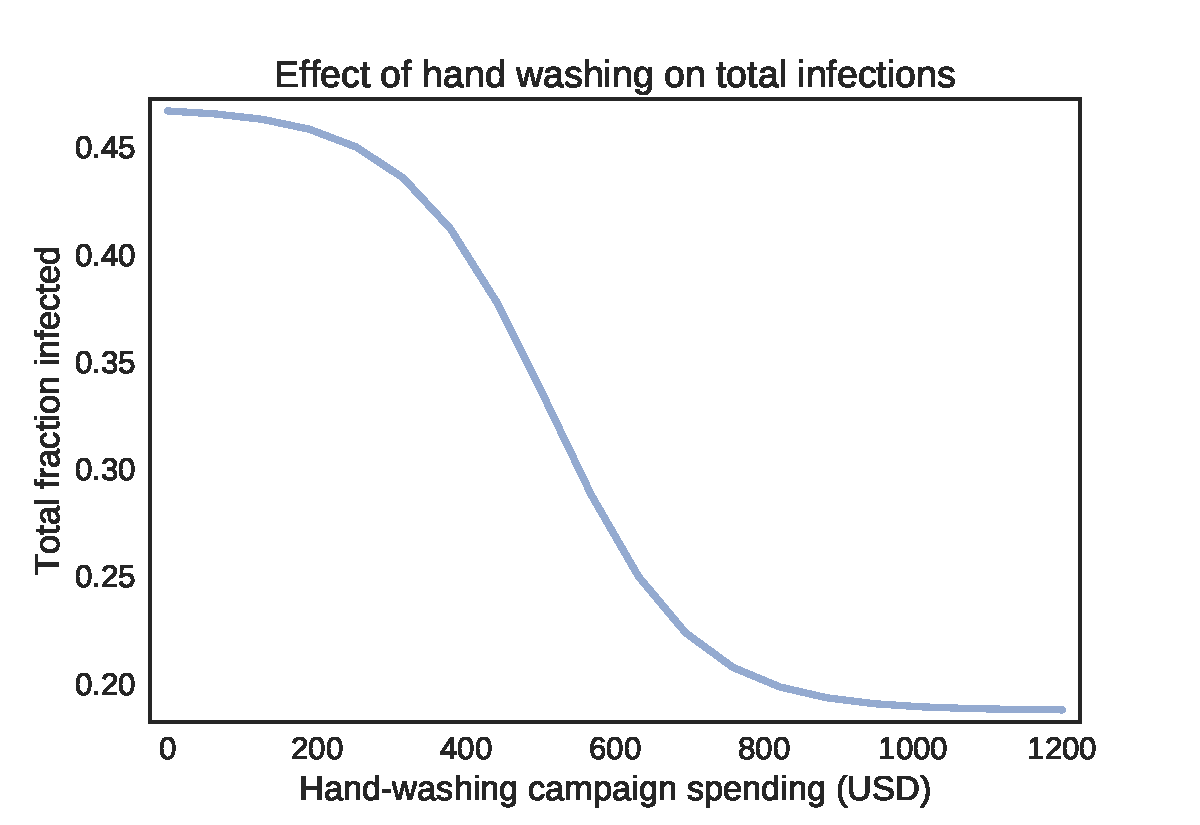
\includegraphics[height=3in]{figs/chap05-fig05.pdf}}
\caption{Fraction of the population infected as a function of hand-washing campaign spending.}
\label{chap05-fig05}
\end{figure} 

Figure~\ref{chap05-fig05} shows the result.  Below \$200, the campaign has little effect.  At \$800 it has a substantial effect, reducing total infections from 46\% to 20\%.  Above \$800, the additional benefit is small.

\section{Optimization} 

Now we can put it altogether.  With a fixed budget of \$1200, we have to decide how many doses of vaccine to buy, at \$100 each, and how much to spend on the hand-washing campaign.

Here are the parameters:

\begin{python}
num_students = 90
budget = 1200
price_per_dose = 100
max_doses = int(budget / price_per_dose)
\end{python}

We'll sweep the range of possible doses:

\begin{python}
dose_array = arange(max_doses+1)
\end{python}

And run the simulation for each dose:

\begin{python}
def sweep_doses(dose_array):
    sweep = Sweep()
    for doses in dose_array:
        fraction = doses / num_students
        spending = budget - doses * price_per_dose
        
        sir = make_system(beta, gamma)
        add_immunization(sir, fraction)
        add_hand_washing(sir, spending)
        
        run_simulation(sir, update1)
        sweep[doses] = calc_total_infected(sir)

    return sweep
\end{python}

For each number of doses, we compute the fraction of students we can immunize, \py{fraction} and the remaining budget we can spend on the campaign, \py{spending}.  Then we run the simulation with those quantities and store the number of infections.

\begin{figure}
\centerline{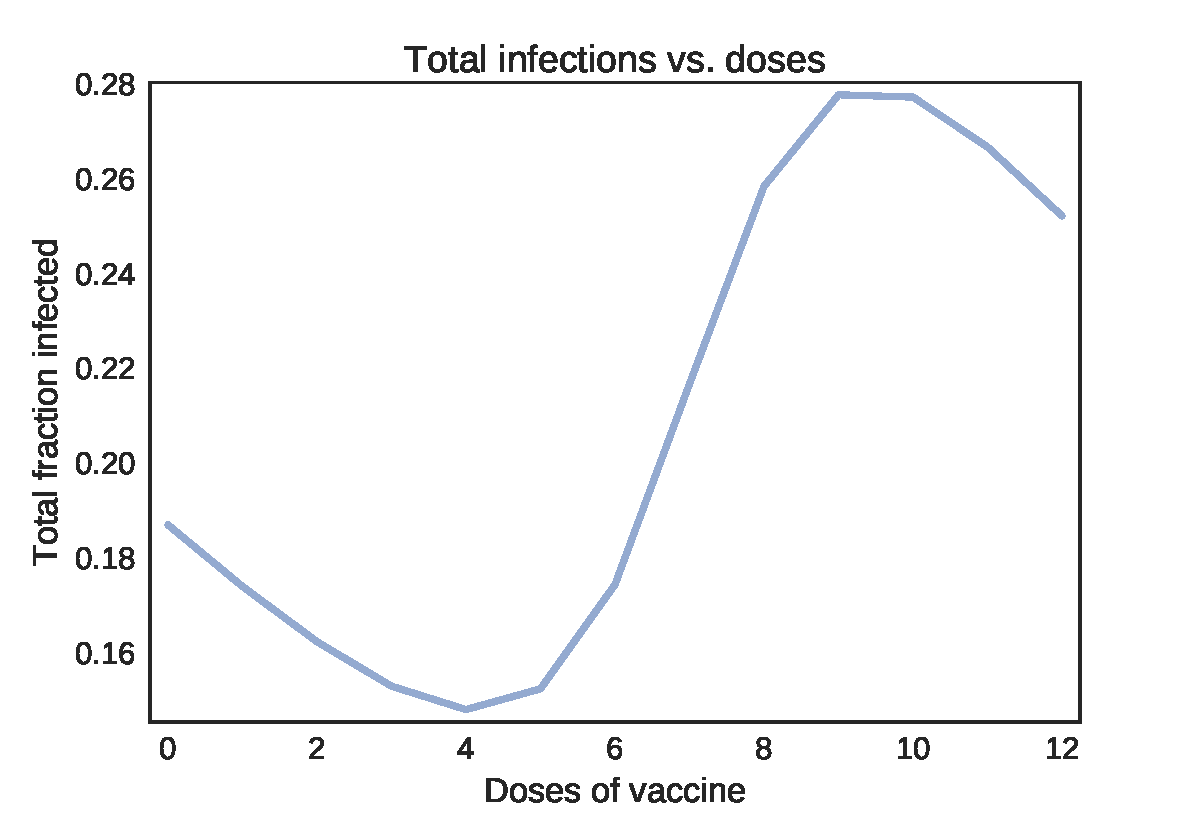
\includegraphics[height=3in]{figs/chap05-fig06.pdf}}
\caption{Fraction of the population infected as a function of the number of doses.}
\label{chap05-fig06}
\end{figure} 

Figure~\ref{chap05-fig06} shows the result.  If we buy no doses of vaccine and spend the entire budget on the campaign, the fraction infected is around 19\%.  At 4 doses, we have \$800 left for the campaign, and this is the optimal point that minimizes the number of students who get sick.

As we increase the number of doses, we have to cut campaign spending, which turns out to make things worse.  But interestingly, when we get above 10 doses, the effect of herd immunity starts to kick in, and the number of sick students goes down again.

In the notebook for this chapter, you'll have a chance to run this optimization for different scenarios.



\chapter{Analysis}

In the previous chapter I presented an SIR model of infectious disease, specifically the Kermack-McKendrick model.  We extended the model to include vaccination and the effect of a hand-washing campaign, and used the extended model to allocate a limited budget optimally, that is, to minimize the number of infections.

But we assumed that the parameters of the model, contact rate and recovery rate, were known.  In this chapter, we explore the behavior of the model as we vary these parameters, use analysis to understand these relationships better, and propose a method for using data to estimate parameters.

We will use the following functions as defined in the previous chapter:
\py{make_system}, \py{run_simulation}, \py{update1}, \py{plot_results}, and \py{calc_total_infected}.

For example, here's the code to create a \py{System} object with given values of \py{beta} and \py{gamma}, run the simulation, and compute the fraction of the population that are infected.

\begin{python}
sir = make_system(0.33, 0.25)
run_simulation(sir, update1)
print(calc_total_infected(sir))
\end{python}


\section{Sweeping beta}

Recall that $\beta$ is the contact rate, which captures both the frequency of interaction between people and the fraction of those interactions that result in a new infection.  If $N$ is the size of the population and $s$ is the fraction that's susceptible, $s N$ is the number of susceptibles, $\beta s N$ is the number of contacts per day between susceptibles and other people, and $\beta s i N$ is the number of those contacts where the other person is infectious.

As $\beta$ increases, we expect the total number of infections to increase.  To quantify that relationship, I'll create a range of values for $\beta$:

\begin{python}
beta_array = linspace(0.1, 0.9, 11)
\end{python}

Then run the simulation for each value and print the results.

\begin{python}
for beta in beta_array:
    sir = make_system(beta, gamma)
    run_simulation(sir, update1)
    print(sir.beta, calc_total_infected(sir))
\end{python}

We can encapsulate that code in a function and store the results in a \py{Sweep} object:

\begin{python}
def sweep_beta(beta_array, gamma):
    sweep = Sweep()
    for beta in beta_array:
        system = make_system(beta, gamma)
        run_simulation(system, update1)
        sweep[system.beta] = calc_total_infected(system)
    return sweep
\end{python}

Now we can run \py{sweep_beta} like this:

\begin{python}
infected_sweep = sweep_beta(beta_array, gamma)
\end{python}

And plot the results:

\begin{python}
label = 'gamma = ' + str(gamma)
plot(infected_sweep, label=label)
\end{python}

%TODO: figure out when to introduce strings

The first line uses string operations to assemble a label for the plotted line:

\begin{itemize}

\item When the \py{+} operator is applied to strings, it joins them end-to-end, which is called {\bf concatenation}.  

\item The function \py{str} converts any type of object to a String representation.  In this case, \py{gamma} is a number, so we have to convert it to a string before trying to concatenate it.

\end{itemize}

If the value of \py{gamma} is \py{0.25}, the value of \py{label} is the string \py{'gamma = 0.25'}.

\begin{figure}
\centerline{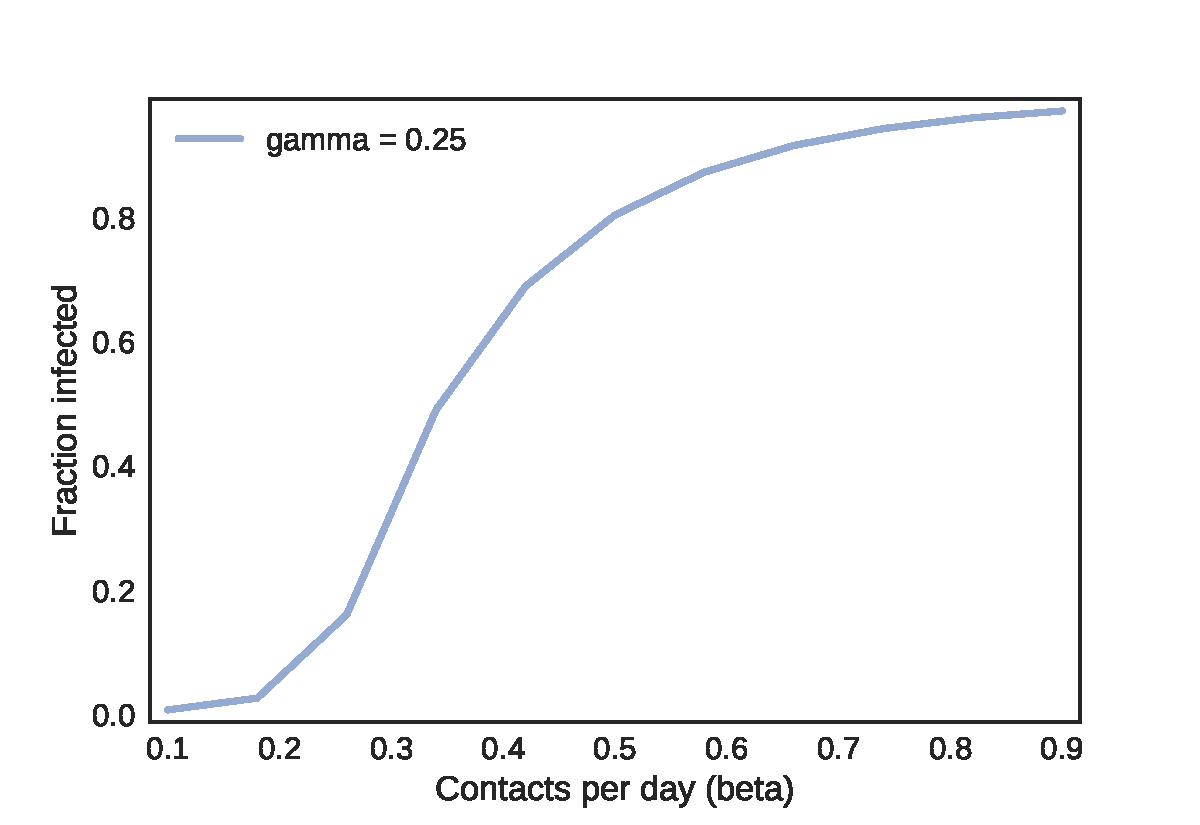
\includegraphics[height=3in]{figs/chap06-fig01.pdf}}
\caption{Total number of infected students as a function of the parameter \py{beta}, with \py{gamma = 0.25}.}
\label{chap06-fig01}
\end{figure}

Figure~\ref{chap06-fig01} shows the results.  Remember that this figure is a parameter sweep, not a time series, so the x-axis is the parameter \py{beta}, not time.  

When \py{beta} is small, the contact rate is low and the outbreak never really takes off; the total number of infected students is near zero.  As \py{beta} increases, it reaches a threshold near 0.3 where the fraction of infected students increases quickly.  When \py{beta} exceeds 0.5, more than 80\% of the population gets sick.


\section{Sweeping gamma}

Now let's see what that looks like for a few different values of \py{gamma}.  Again, we'll use \py{linspace} to make an array of values:

\begin{python}
gamma_array = linspace(0.1, 0.7, 4)
\end{python}

And run \py{sweep_beta} for each value of \py{gamma}:

\begin{python}
for gamma in gamma_array:
    infected_sweep = sweep_beta(beta_array, gamma)
    label = 'gamma = ' + str(gamma)
    plot(infected_sweep, label=label)
\end{python}

\begin{figure}
\centerline{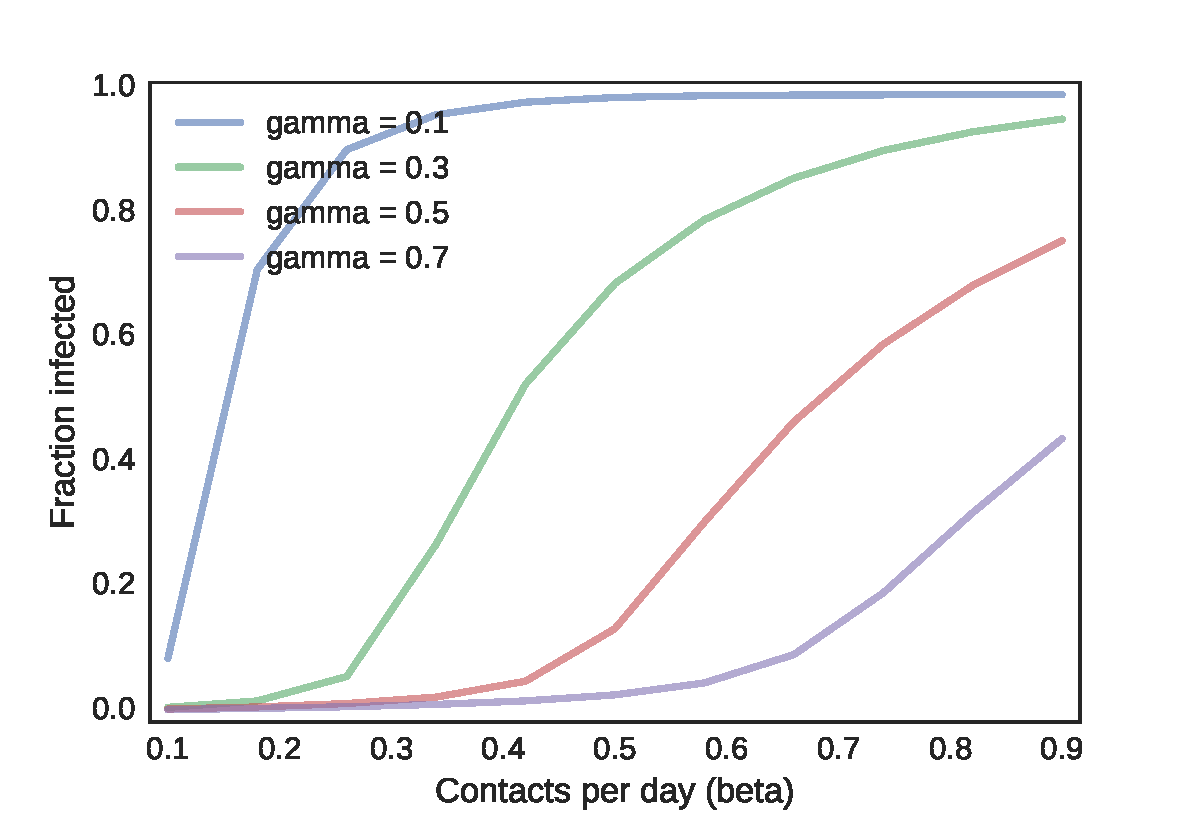
\includegraphics[height=3in]{figs/chap06-fig02.pdf}}
\caption{Total number of infected students as a function of the parameter \py{beta}, for several values of \py{gamma}.}
\label{chap06-fig02}
\end{figure}

Figure~\ref{chap06-fig02} shows the results.  When \py{gamma} is low, the recovery rate is low, which means people are infectious longer.  In that case, even low a contact rate (\py{beta}) results in an epidemic.

When \py{gamma} is high, \py{beta} has to be even higher to get things going.  That observation suggests that there might be a relationship between \py{gamma} and \py{beta} that determines the outcome of the model.  

In fact, there is.  I will demonstrate it first by running simulations, then derive it by analysis.


\section{Nondimensionalization}

Before we go on, let's encapsulate the code from the previous section in a function:

\begin{python}
def sweep_parameters(beta_array, gamma_array):
    sf = SweepFrame(columns=gamma_array)
    for gamma in gamma_array:
        sf[gamma] = sweep_beta(beta_array, gamma)
    return sf
\end{python}

\py{sweep_parameters} takes as parameters two arrays: a range of values for \py{beta} and a range of values for \py{gamma}.

It creates a \py{SweepFrame} to store the results, with one column for each value of \py{gamma} and one row for each value of \py{beta}.  A \py{SweepFrame} is a kind of \py{DataFrame}, defined in \py{modsim.py}.  Its purpose is to store results from a two-dimensional parameter sweep.

Each time through the loop, we run \py{sweep_beta}.  The result is a \py{Sweep} object with one element for each value of \py{gamma}.  The assignment

\begin{python}
sf[gamma] = sweep_beta(beta_array, gamma)
\end{python}

stores the values from the \py{Sweep} object as a new column in the \py{SweepFrame}, corresponding to the current value of \py{gamma}.

At the end, the \py{SweepFrame} stores the fraction of students infected for each pair of parameters, \py{beta} and \py{gamma}.

We can run it like this:

\begin{python}
sf = sweep_parameters(beta_array, gamma_array)
\end{python}

Then we can loop through the results like this:

\begin{python}
for gamma in sf.columns:
    sweep = sf[gamma]
    for beta in sweep.index:
        frac_infected = sweep[beta]
        print(beta, gamma, frac_infected)
\end{python}

This is the first example we've seen with one \py{for} loop inside another:

\begin{itemize}

\item Each time the outer loop runs, it selects a value of \py{gamma} from the columns of the \py{DataFrame} and extracts the corresponding column.

\item Each time the inner loop runs, it selects a value of \py{beta} from the \py{Sweep} and selects the corresponding element, which is the fraction of student infected.

\end{itemize}  

In this example, \py{sf} has 4 columns, one for each value of \py{gamma}, and 11 rows, one for each value of \py{beta}.  So these loops print 44 lines, one for each pair of parameters.

Now let's think about possible relationships between \py{beta} and \py{gamma}:

\begin{itemize}

\item When \py{beta} exceeds \py{gamma}, that means there are more contacts (that is, potential infections) than recoveries.  The difference between \py{beta} and \py{gamma} might be called the ``excess contact rate", in units of contacts per day.

\item As an alternative, we might consider the ratio \py{beta/gamma}, which is the number of contacts per recovery.  Because the numerator and denominator are in the same units, this ratio is {\bf dimensionless}, which means it has no units.

\end{itemize}

Describing physical systems using dimensionless parameters is often a useful move in the modeling and simulation game.  It is so useful, in fact, that it has a name: nondimensionalization (see \url{https://en.wikipedia.org/wiki/Nondimensionalization#First_order_system}).

So we'll try the second option first.  In the notebook for this chapter, you will explore the first option as an exercise.

The following function encapsulates the previous loops and plots the fraction infected as a function of the ratio \py{beta/gamma}:

\begin{python}
def plot_sweep_frame(sf):
    for gamma in sf.columns:
        sweep = sf[gamma]
        for beta in sweep.index:
            frac_infected = sweep[beta]
            plot(beta / gamma, frac_infected, 'ro')
\end{python}

\begin{figure}
\centerline{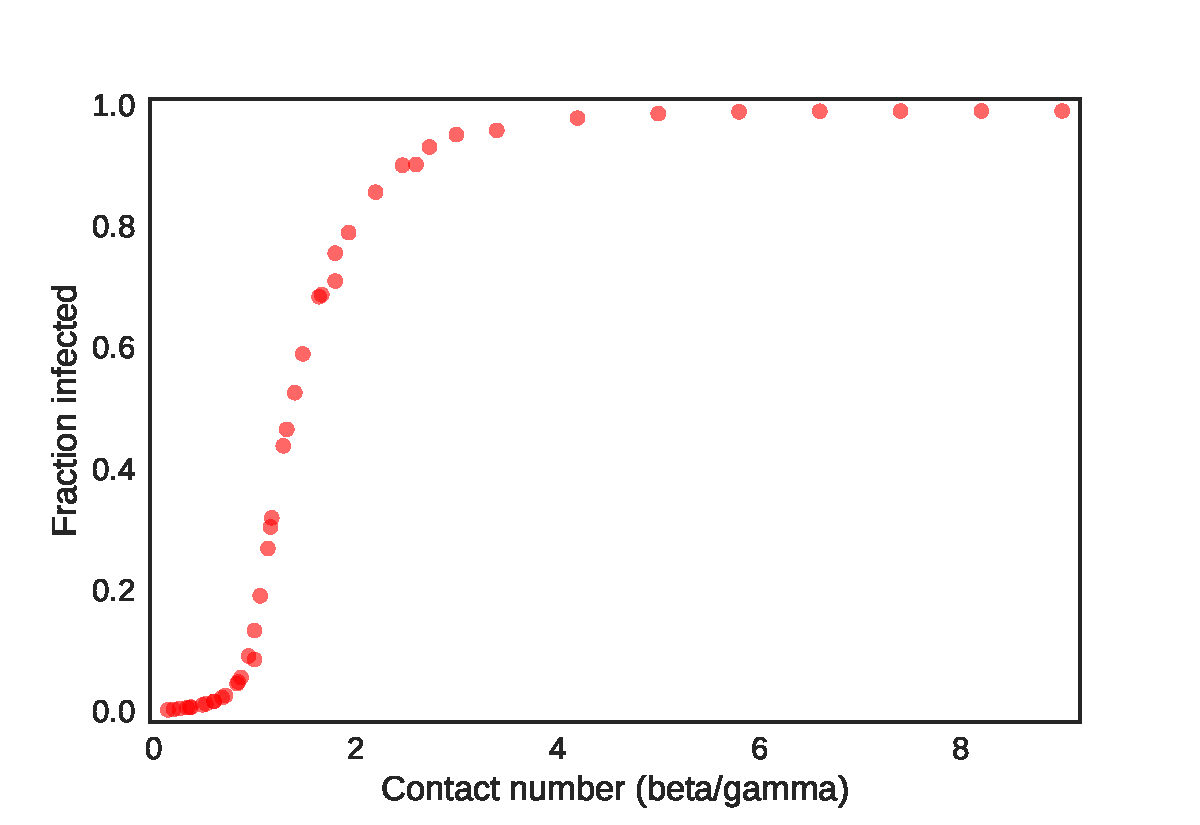
\includegraphics[height=3in]{figs/chap06-fig03.pdf}}
\caption{Total fraction infected as a function of contact number.}
\label{chap06-fig03}
\end{figure}

Figure~\ref{chap06-fig03} shows that the results fall neatly on a single curve, at least approximately.  That means that we can predict the fraction of students who will be infected based on a single parameter, the ratio \py{beta/gamma}.  We don't need to know the values of \py{beta} and \py{gamma} separately.


\section{Contact number}

Recall that the number of new infections in a given day is $\beta s i N$, and the number of recoveries is $\gamma i N$.  If we divide these quantities, the result is $\beta s / \gamma$, which is the number of new infections per recovery (as a fraction of the population).

When a new disease is introduced to a susceptible population, $s$ is approximately 1, so the number of people infected by each sick person is $\beta / \gamma$.  This ratio is called the ``contact number" or ``basic reproduction number" (see \url{https://en.wikipedia.org/wiki/Basic_reproduction_number}).  By convention it is usually denoted $R_0$, but in the context of an SIR model, this notation is confusing, so we'll use $c$ instead.

The results in the previous section suggest that there is a relationship between $c$ and the total number of infections.  We can derive this relationship by analyzing the differential equations from Section~\ref{sireqn}:
%
\begin{align*}
\frac{ds}{dt} &= -\beta s i \\
\frac{di}{dt} &= \beta s i - \gamma i\\
\frac{dr}{dt} &= \gamma i
\end{align*}
%
In the same way we divided the contact rate by the infection rate to get the dimensionless quantity $c$, now we'll divide $di/dt$ by $ds/dt$ to get an equation that does not depend on time:
%
\[ \frac{di}{ds} = -1 + \frac{1}{cs} \]
%
Dividing one differential equation by another is not an obvious move, but in this case it is useful because it gives us a relationship between $i$, $s$ and $c$ that does not depend on time.  We can multiply both sides by $ds$:
%
\[ di = \left( -1 + \frac{1}{cs} \right) ds \]
%
And then integrate both sides:
%
\[ i = -s + \frac{1}{c} \log s + q \]
%
where $q$ is a constant of integration.  Rearranging terms yields:
%
\[ q = i + s - \frac{1}{c} \log s \]
%
Now let's see if we can figure out what $q$ is.  At the beginning of an epidemic, if the fraction infected is small and nearly everyone is susceptible, we can use the approximations $i(0) = 0$ and $s(0) = 1$ to compute $q$:
%
\[ q = 0 + 1 + \frac{1}{c} \log 1 \]
%
Since $\log 1 = 0$, we get $q = 1$.

\newcommand{\sinf}{s_{\infty}}

Now, at the end of the epidemic, let's assume that $i_{\infty} = 0$ and $s(\infty)$ is an unknown quantity $\sinf$.  Now we have:
%
\[ q = 1 = 0 + \sinf - \frac{1}{c} \log \sinf \]
%
Solving for $c$, we get
%
\[ c = \frac{\log \sinf}{\sinf - 1} \]
%
If we create a range of values for $\sinf$

\begin{python}
s_inf_array = linspace(0.0001, 0.9999, 31)
\end{python}

we can compute the corresponding values of $c$:

\begin{python}
c_array = np.log(s_inf_array) / (s_inf_array - 1)
\end{python}

To get the total infected, we compute the difference between $s(0)$ and $s(\infty)$, then store the results in a \py{Series}:

\begin{python}
frac_infected = 1 - s_inf_array
frac_infected_series = Series(frac_infected, index=c_array)
\end{python}

Recall from Section~\ref{series} that a \py{Series} object contains an index, which is \py{c_array} in this example, and a corresponding sequence of values, which is \py{frac_infected}.


\section{Analysis and simulation}

Now we can plot the results:

\begin{python}
plot(frac_infected_series)
\end{python}

\begin{figure}
\centerline{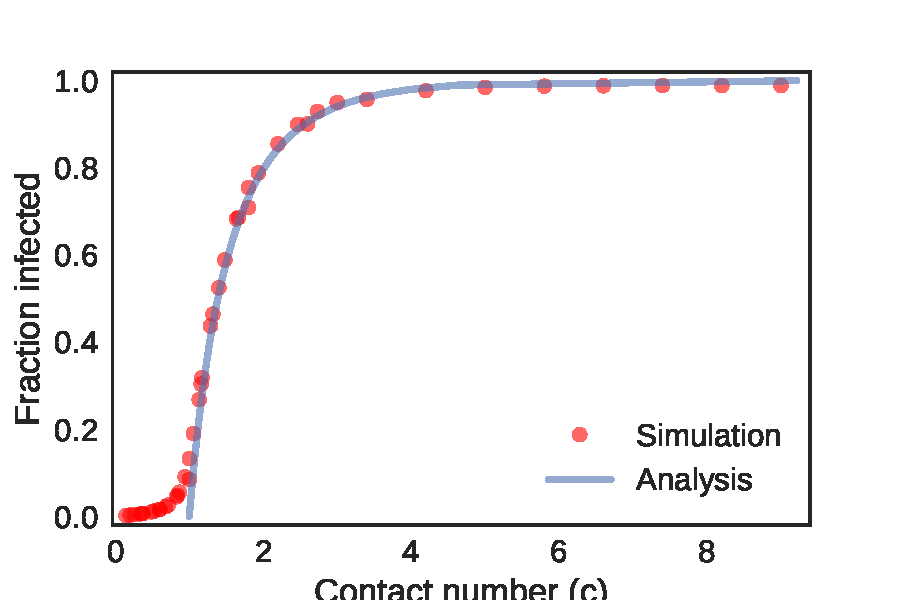
\includegraphics[height=3in]{figs/chap06-fig04.pdf}}
\caption{Total fraction infected as a function of contact number, results from simulation and analysis.}
\label{chap06-fig04}
\end{figure}

Figure~\ref{chap06-fig04} compares the analytic results from this section with the simulation results from the previous section.  Over most of the range they are consistent with each other, but when the contact number is less than 1, the analysis suggests that there will be virtually no infections; in the simulations a new infection can affect a small part of the population, even when $c<1$.

The reason for the discrepancy is that the simulation divides time into a discrete series of days, whereas the analysis treats time as a continuous quantity.  In other words, the two methods are actually based on different models.

So which model is better?  Probably neither.  When the contact number is small, the early progress of the epidemic will depend on details of the scenario.  If we are lucky, the original infected person, ``patient zero",  infects no one and there is no epidemic.  If we are unlucky, patient zero might have a large number of close friends, or might work in the dining hall (and fail to observe safe food handling procedures).

For contact numbers near or less than 1, we might need a more detailed model.  But for higher contact numbers the SIR model might be good enough.

Figure~\ref{chap06-fig04} shows that if we know the contact number, we can compute the fraction infected.  But we can also read the figure the other way; that is, at the end of an epidemic, if we can estimate the fraction of the population that was ever infected, we can use it to estimate the contact number.

Well, at least in theory.  In practice, it might not work very well, because of the shape of the curve.  When the contact number is near 2, the curve is quite steep, which means that small changes in $c$ yield big changes in the number of infections.  If we observe that the total fraction infected is anywhere from 20\% to 80\%, we would conclude that $c$ is near 2.

On the other hand, for larger contact numbers, nearly the entire population is infected, so the curve is quite flat.  In that case we would not be able to estimate $c$ precisely, because any value greater than 3 would yield effectively the same results.  Fortunately, this is unlikely to happen in the real world; very few epidemics affect anything like 90\% of the population.

In summary, the SIR model has limitations; nevertheless, it provides insight into the behavior of infectious disease, especially the phenomenon of herd resistance.  As we saw in the previous chapter, if we know the parameters of the model, we can use it to evaluate possible interventions.  And as we saw in this chapter, we might be able to use data from earlier outbreaks to estimate the parameters.



\chapter{Thermal systems}

Intro

\section{The coffee cooling problem}

The coffee cooling problem was discussed by Jearl Walker in Scientific American in 1977\footnote{Walker, ``The Amateur Scientist", Scientific American, Volume 237, Issue 5, November 1977.}, and since then it has become a standard example of modeling and simulation.

Here is my version of the problem:

\begin{quote}
Suppose I stop on the way to work to pick up a cup of coffee, which I take with milk.  Assuming that I want the coffee to be as hot as possible when I arrive at work, should I add the milk at the coffee shop, wait until I get to work, or add the milk at some point in between?
\end{quote}

To help answer this question, I made a trial run with the milk and coffee in separate containers and took some measurements:

\begin{itemize}

\item When served, the temperature of the coffee is \SI{90}{\celsius}.  The volume is \SI{300}{mL}.

\item The milk is at an initial temperature of \SI{5}{\celsius}, and I take about \SI{50}{mL}.

\item The ambient temperature in my car is \SI{22}{\celsius}.

\item The coffee is served in a well insulated cup.  When I arrive at work after 30 minutes, the temperature of the coffee has fallen to \SI{70}{\celsius}.

\item The milk container is not as well insulated.  After 15 minutes, it warms up to \SI{20}{\celsius}, nearly the ambient temperature.

\end{itemize}

To use this data and answer the question, we'll need to know something about temperature and heat, and we'll have to make some modeling decisions.


\section{Temperature and heat}

To understand how coffee cools (and milk warms), we need a model of temperature and heat.  {\bf Temperature} is a property of an object or a system; it quantifies how hot or cold the object is, which is related to the average velocity of the particles that make up the object.  As an object cools, its particles slow down.

{\bf Heat} is a flow of energy from one object to another.  As the coffee cools, heat flows from the coffee, through the container, and into the surrounding environment.

Heat is related to temperature by the following equation (see \url{https://en.wikipedia.org/wiki/Thermal_mass}):
%
\[ Q = C \Delta T \]
%
where $Q$ is the amount of heat transferred to an object, usually measured in joules (\si{J}), $\Delta T$ is the change in temperature of the object, measured in degrees Celsius (\si{\celsius}), and $C$ is the {\bf thermal mass} of the object which quantifies how much energy it takes to heat or cool it, in joules per degree Celsius (\si{J/\celsius}).

For objects made primarily from one material, thermal mass can be computed like this:
%
\[ C = m c_p \]
%
where $m$ is the mass of the object and $c_p$ is the {\bf specific heat capacity} of the material (see \url{https://en.wikipedia.org/wiki/Heat_capacity#Specific_heat_capacity}).

The specific heat capacity of coffee is probably close to that of water, which is \SI{4.2}{J/g/\celsius}.

Assuming that the density of coffee is close to that of water, which is \SI{1}{g/ml}, the mass of \SI{300}{mL} of coffee is \SI{300}{g}, and the thermal mass is \SI{1260}{J/\celsius}.  So when the coffee cooled from \SI{90}{\celsius} to \SI{70}{\celsius}, the change in temperature, $\Delta T$ was \SI{20}{\celsius}, which means that \SI{25200}{J} of heat energy was transferred from the coffee to the surrounding environment, presumably the cup holder and air in my car.

To give you a sense of how much energy that is, if you were able to harness all of that heat to do work (which you cannot), you could use it to lift a cup of coffee from sea level to \SI{8571}{m}, just shy of the height of Mount Everest, \SI{8848}{m}.

Assuming that the cup has less mass than the coffee, and is made from a material with lower a specific heat, we can ignore the thermal mass of the cup.


\section{Heat transfer}

In a situation like the coffee cooling problem, there are three ways heat flows from one object to another (see \url{https://en.wikipedia.org/wiki/Heat_transfer}):

\begin{itemize}

\item Conduction: When objects at different temperatures come into contact, the faster-moving particles of the higher-temperature object transfer kinetic energy to the slower-moving particles of the lower-temperature object.  This energy transfer is a form of heat flow.

\item Convection: When particles in a gas or liquid flow from place to place, they carry heat energy with them.  Fluid flows can be caused by external action, like stirring, or by internal differences in temperature.  For example, you might have heard that hot air rises, which is a form of ``natural convection".

\item Radiation: As the particles in an object move due to thermal energy, they emit electromagnetic radiation.  The heat energy carried by this radiation depends on the object's temperature and surface properties, including its {\bf emissivity} (see \url{https://en.wikipedia.org/wiki/Thermal_radiation}).

\end{itemize}

For objects like coffee in a car, thermal radiation is much smaller than 
heat transfer due to conduction and convection, so we will ignore it.

Convection can be a complex topic, since it often depends on details of fluid flow in three dimensions.  But for this problem we will be able to get away with a simple model called ``Newton's law of cooling".


\section{Newton's law of cooling}

Newton's law of cooling asserts that the temperature rate of change for an object is proportional to the difference in temperature between the object and the surrounding environment:
%
\[ \frac{dT}{dt} = -r (T - T_{env}) \]
%
where $T$, the temperature of the object, is a function of time, $t$; $T_{env}$ is the temperature of the environment, and $r$ is a constant that characterizes how quickly heats moves between across the boundary between the system and the environment.

Newton's so-called ``law" is really a model in the sense that it is approximately true in some conditions, only roughly true in others, and not at all true in others.

For example, if the primary mechanism of heat transfer is conduction, Newton's law is ``true", which is to say that $r$ is constant over a wide range of temperatures.  And sometimes we can estimate $r$ based on the material properties and shape of the object.

When convection contributes a non-negligible fraction of heat transfer, $r$ might depend on temperature, but Newton's law is often accurate enough, at least over some range of temperatures.  In this case $r$ usually has to be estimated experimentally, since it depends on details of surface shape, air flow, evaporation, etc.

When radiation makes up a substantial part of heat transfer, Newton's law is not a good model at all.  This is the case for objects in space or in a vacuum, and for objects at high temperatures, more than a few hundred degrees Celsius, say.

However, for a situation like the coffee cooling problem, we expect Newton's model to be quite good.


\section{Implementation}

To get started, let's forget about the milk temporarily and focus on the coffee.  I'll create a \py{State} object to represent the initial temperature:

\begin{python}
init = State(temp=90)
\end{python}

And a \py{System} object to contain the parameters of the system:

\begin{python}
coffee = System(init=init, T_env=22, r=0.01,
                t0=0, t_end=30, dt=1)
\end{python}

The values of \py{T_env}, \py{t0}, and \py{t_end} come from the statement of the problem.  I chose the value of \py{r} arbitrarily for now; we will figure out how to estimate it soon.

\py{dt} is the time step we'll use to simulate the cooling process.
Strictly speaking, Newton's law is a differential equation, but over a short period of time we can approximate it with a difference equation:
%
\[ \Delta T = -r (T - T_{env}) \Delta t \]
%
where $\Delta t$ is a small time step and $\Delta T$ is the change in temperature during that time step.

One note: I use $\Delta T$ to denote a change in temperature over time, but in the context of heat transfer, you might also see $\Delta T$ used to denote the difference in temperature between an object and its environment, $T - T_{env}$.  To minimize confusion, I will avoid this second use.

%TODO: introduce unpack()

Now we can write an update function:

\begin{python}
def update(system, state):
    T = state.temp
    dT = - system.r * (T - system.T_env) * system.dt
    return State(temp=T+dT)
\end{python}

Now if we run 

\begin{python}
update(coffee, init)
\end{python}

we see that the temperature after one minute is \SI{89.3}{\celsius}, so the temperature drops by about \SI{0.7}{\celsius\per\minute}, at least for this value of \py{r}.

Now we can use \py{run_simulation}, as defined in Section~\ref{timeframe}, to simulate a series of time steps from \py{t0} to \py{t_end}:

\begin{python}
def run_simulation(system, update_func):
    df = TimeFrame(columns=system.init.index)
    df.loc[system.t0] = system.init
    
    for i in range(system.t0, system.t_end):
        df.loc[i+1] = update_func(system, df.loc[i])
    
    system.results = df
\end{python}

and run it like this:

\begin{python}
run_simulation(coffee, update)
\end{python}

The result is a \py{TimeFrame} object with one row per time step and just one column, \py{temp}.  The temperature after 30 minutes is \SI{72.3}{\celsius}, which is a little higher than stated in the problem, \SI{70}{\celsius}.  We could adjust \py{r} by hand and find the right value by trial and error, but we can do better, as we'll see in the next section.

First I want to encapsulate what we have so far in a function:

\begin{python}
def run(T_init, **kwargs):
    init = State(temp=T_init)
    system = System(init=init, T_env=22, t0=0, 
                    dt=1, **kwargs)
    run_simulation(system, update)
    return system
\end{python}

\py{run} uses a feature we have not seen before: the parameter \py{**kwargs} gathers any keyword arguments provided when the function runs and stores them in an object (specifically, it's a Python dictionary).

In this example, it passes the arguments along to \py{System}, so they become variables in the new \py{System} object.

If we call it like this:

\begin{python}
coffee = run(T_init=90, t_end=30, r=0.01)
\end{python}

\py{coffee} contains \py{t_end} and \py{r} as system variables, along with
\py{init}, \py{T_env}, \py{t0}, and \py{dt}.

Now let's see a better was to estimate \py{r}.


\section{Using fsolve}

SciPy provides a method called \py{fsolve} that finds the roots of non-linear equations.  As a simple example, suppose you want to find the roots of the polynomial
%
\[ f(x) = (x - 1)(x - 2)(x - 3) \]
%
where ``root" means a value of $x$ that makes $f(x)=0$.  Because of the way I wrote the polynomial, we can see that if $x=1$, the first factor is 0; if $x=2$, the second factor is 0; and if $x=3$, the third factor is 0, so those are the roots.

But usually it's not that easy.  In that case \py{fsolve} can help.  First, we have to write a function that evaluates $f$:

\begin{python}
def func(x):
    return (x-1) * (x-2) * (x-3)
\end{python}

Now we call \py{fsolve} like this:

\begin{python}
fsolve(func, x0=0)
\end{python}

The first argument is the function whose roots we want.  The second argument, \py{x0}, is an initial guess about where a root might be.  Generally, the closer the initial guess is to an actual root, the faster \py{fsolve} runs.  In this case, with the initial guess \py{x0=0}, the result is 1.

Often \py{fsolve} finds the root that's closest to the initial guess.  In this example, when \py{x0=1.9}, \py{fsolve} returns 2, and when \py{x0=2.9}, \py{fsolve} returns 3.  But this behavior can be unpredictable; with \py{x0=1.5}, \py{fsolve} returns 3.

So how can we use \py{fsolve} to estimate \py{r}?  

Now, we want to find the value of \py{r} that yields a final temperature of \SI{70}{\celsius}.  To work with \py{fsolve}, we need a function that takes \py{r} as a parameter and returns the difference between the final temperature and the goal:

\begin{python}
def error_func1(r):
    system = run(T_init=90, t_end=30, r=r)
    return final_temp(system) - 70
\end{python}

I call a function like this an ``error function" because it returns the difference between what we got and what we wanted, that is, the error.  When we find the right value of \py{r}, this error will be 0.

We can test \py{error_func1} like this, using our initial guess for \py{r}:

\begin{python}
error_func1(r=0.01)
\end{python}

The result is an error of \SI{2.3}{\celsius}, because the final temperature with this value of \py{r} is too high.

Now we can call \py{fsolve} like this:

\begin{python}
solution = fsolve(error_func1, 0.01)
r_coffee = solution[0]
\end{python}

The return value from \py{fsolve} is an array with a single element, which is the root \py{fsolve} found.  In this example, \py{r_coffee} turns out to be about \py{0.012}, in units of \si{\per\minute}.

\begin{figure}
\centerline{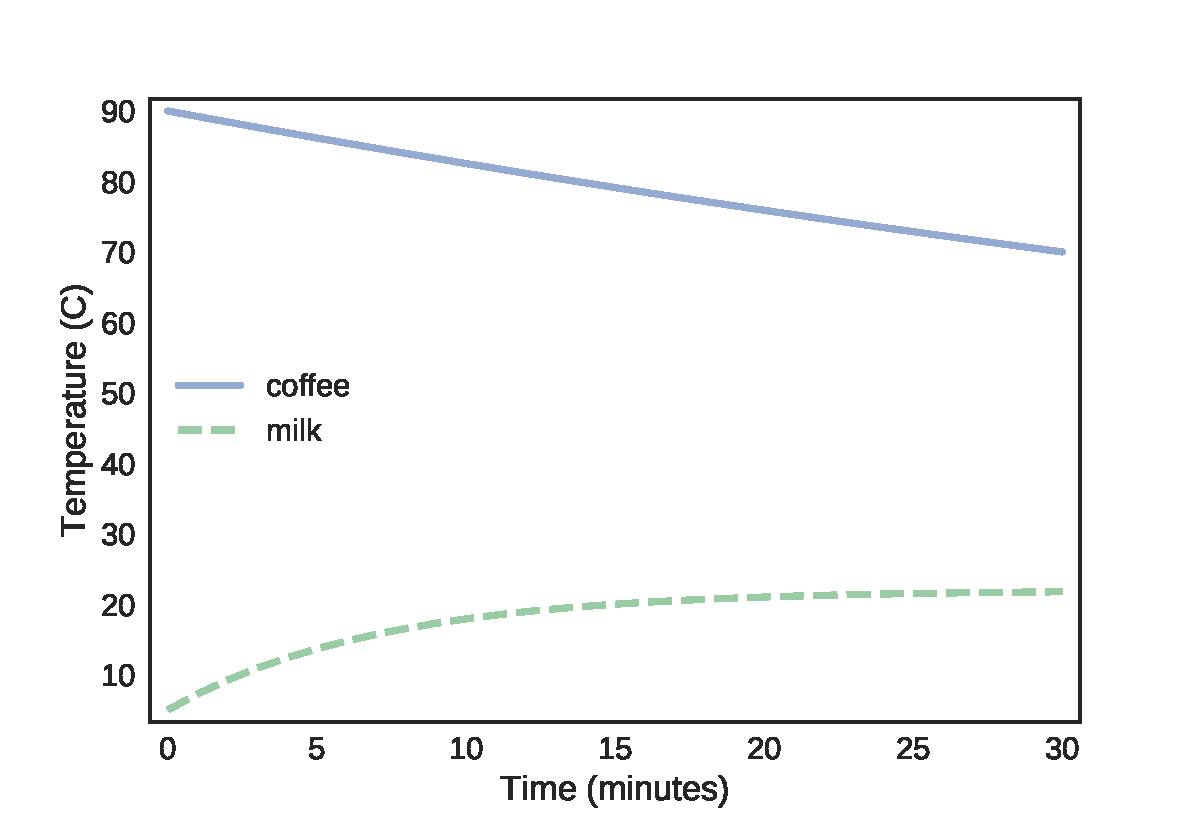
\includegraphics[height=3in]{figs/chap07-fig01.pdf}}
\caption{Temperature of the coffee and milk over time.}
\label{chap07-fig01}
\end{figure}

As one of the exercises for this chapter, you will use the same process to estimate \py{r_milk}.  The result should look like Figure~\ref{chap07-fig01}, which shows the temperature of the coffee and milk over time, with the estimated values of \py{r_coffee} and \py{r_milk}.


\section{Mixing liquids}

When we mix two liquids, the temperature of the mixture depends on the temperatures of the ingredients, but it might not be obvious how to compute it.

Assuming there are no chemical reactions between the liquids that either produce or consume heat, the total thermal energy of the system is the same before and after mixing; in other words, thermal energy is {\bf conserved}.

If the temperature of the first liquid is $T_1$, the temperature of the second liquid is $T_2$, and the final temperature of the mixture is $T$, the heat transfer into the first liquid is $C_1 (T - T_1)$ and the heat transfer into the second liquid is $C_2 (T - T_2)$, where $C_1$ and $C_2$ are the thermal masses of the liquids.

In order to conserve energy, these heat transfers must add up to 0:
%
\[ C_1 (T - T_1) + C_2 (T - T_2) = 0 \]
%
We can solve this equation for T:
%
\[ T = \frac{C_1 T_1 + C_2 T_2}{C_1 + C_2} \]
%
For the coffee cooling problem, we have the volumes of the liquids; to get their thermal masses, recall that thermal mass is related to mass, $m$, by specific heat capacity, $c_p$:
%
\[ C = m c_p \]
%
And mass is related to volume $V$, by density, $\rho$ (see \url{https://en.wikipedia.org/wiki/Density}):
%
\[ m = \rho V \]
%
So the thermal mass of each ingredient is
%
\[ C = \rho V c_p \]
%
If we assume that the density and specific heat of the milk and coffee are equal, they drop out of the equation, and we can write:
%
\[ T = \frac{V_1 T_1 + V_2 T_2}{V_1 + V_2} \]
%
where $V_1$ and $V_2$ are the volumes of the liquids.  As an exercise, you can look up the density and specific heat of milk to see how good this approximation is.

The following function takes two \py{System} objects that represent the coffee and milk, creates a new \py{System} to represent the mixture, then runs a simulation of the mixture until \py{t_end}.  The return value is the new \py{System}.

\begin{python}
def mix(s1, s2, t_end):
    assert s1.t_end == s2.t_end
    
    volume = s1.volume + s2.volume
    
    temp = (s1.volume * final_temp(s1) + 
            s2.volume * final_temp(s2)) / volume
    
    mixture = run(T_init=temp, t_end=t_end, 
                  r=s1.r, volume=volume)
    return mixture
\end{python}

The first line is an \py{assert} statement, which is a way of checking for errors.  It compares \py{t_end} for the two systems to confirm that they have been cooling for the same time.  If not, \py{assert} displays an error message and stops the program.

The next two statements compute the total volume of the mixture and its temperature.  Then we use \py{run} to make a new \py{System} and simulate it.

This function uses the value of \py{r} from \py{s1} as the value of \py{r} for the mixture.  If \py{s1} represents the coffee, and we are adding the milk to the coffee, this is probably a reasonable choice.  On the other hand, when we increase the amount of liquid in the coffee cup, that might change \py{r}.  So this is an assumption to revisit when we consider sources of error.


\section{Mix first or last?}

Now we have everything we need to solve the problem.  First I'll create objects to represent the coffee and cream, and run for 30 minutes.

\begin{python}
coffee = run(T_init=90, t_end=30, r=r_coffee, volume=300)
milk = run(T_init=5, t_end=30, r=r_milk, volume=50)
\end{python}

The final temperatures, before mixing, are \SI{70}{\celsius} and \SI{21.7}{\celsius}.  Then we mix them:

\begin{python}
mix_last = mix(coffee, milk)
\end{python}

After mixing, the temperature is \SI{63.1}{\celsius}, which is still warm enough to be enjoyable.  Would we do any better if we added the milk first?

I'll create new objects for the coffee and milk, with \py{t_end=0}

\begin{python}
coffee = run(T_init=90, t_end=0, r=r_coffee, volume=300)
milk = run(T_init=5, t_end=0, r=r_milk, volume=50)
\end{python}

Then mix them and simulate 30 minutes:

\begin{python}
mix_first = mix(coffee, milk, t_end=30)
\end{python}

The final temperature is only \SI{61.6}{\celsius}.  So it looks like adding the milk at the end is better, by about \SI{1.5}{\celsius}.  But is that the best we can do?


\section{Optimization}

Adding the milk after 30 minutes is better than adding it after one minute, but maybe there's something in between that's even better.  To find out, I'll use the following function, which takes \py{t_add} as a parameter:

\begin{python}
def run_and_mix(t_add):
    coffee = run(T_init=90, t_end=t_add, 
                 r=r_coffee, volume=300)
    milk = run(T_init=5, t_end=t_add, 
               r=r_milk, volume=50)
    mixture = mix(coffee, milk, t_end=30-t_add)
    return final_temp(mixture)
\end{python}

When \py{t_add=0}, we add the milk immediately; when \py{t_add=30}, we add it at the end.  Now we can sweep the range of values in between:

\begin{python}
sweep = Sweep()
for t_add in arange(0, 30):
    temp = run_and_mix(t_add)
    sweep[t_add] = temp
\end{python}

\begin{figure}
\centerline{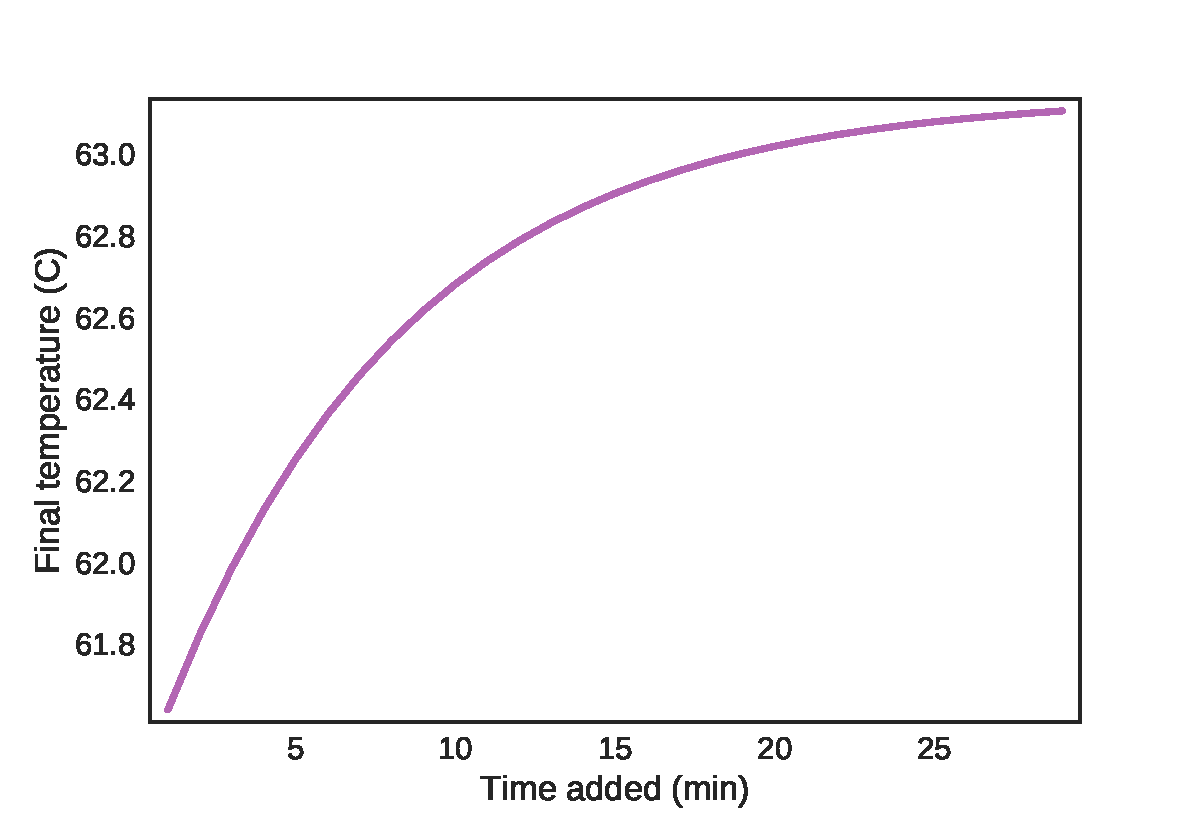
\includegraphics[height=3in]{figs/chap07-fig02.pdf}}
\caption{Final temperature as a function of when we add the milk.}
\label{chap07-fig02}
\end{figure}

Figure~\ref{chap07-fig02} shows the result.  Again, note that this is a parameter sweep, not a time series.  The x-axis is the time when we add the milk, not the time index of a \py{TimeSeries}.

The final temperature is maximized when \py{t_add=30}, so adding the milk at the end is optimal.

In the notebook for this chapter you will have a chance to explore this solution and try some variations.  For example, suppose the coffee shop won't let me take milk in a separate container, but I keep a bottle of milk in the refrigerator at my office.  In that case is it better to add the milk at the coffee shop, or wait until I get to the office?


\section{Analysis}

Simulating Newton's law of cooling is almost silly, because we can solve the differential equation analytically.  If
%
\[ \frac{dT}{dt} = -r (T - T_{env}) \]
%
the general solution is
%
\[ T{\left (t \right )} = C_{1} e^{- r t} + T_{env} \]
%
and the particular solution where $T(0) = T_init$ is
%
\[ T_{env} + \left(- T_{env} + T_{init}\right) e^{- r t} \]
%
In the notebook for this chapter, you'll see how I got this solution using SymPy, and if you would like to see it done by hand, you can watch this video: \url{https://www.khanacademy.org/math/ap-calculus-ab/diff-equations-ab/exponential-models-ab/v/newtons-law-of-cooling}

Now we can use the observed data to estimate the parameter $r$.  If we observe $T(t_{end}) = T_{end}$, we can plug $t_{end}$ and $T_{end}$ into the particular solution and solve for $r$.  The result is:
%
\[ r = \frac{1}{t_{end}} \log{\left (\frac{T_{init} + T_{env}}{T_{end} - T_{env}} \right )} \]
%
Plugging in $t_{end}=30$ and $T_{end}=70$ (and again with $T_{init}=90$ and $T_{env}=22$), the estimate for $r$ is 0.0116.

We can use this function to compute the time series:

\begin{python}
def run_analysis(system):
    T_init = system.init.temp
    T_env = system.T_env
    
    ts = arange(system.t0, system.t_end+1)
    Ts = T_env + (T_init - T_env) * np.exp(-system.r * ts)
    series = TimeSeries(Ts, index=ts)
    
    system.results = TimeFrame(series, columns=['temp'])
\end{python}

The interface for this function is similar to \py{run_simulation}: it takes a \py{System} as a parameter, and stores a \py{TimeFrame} as a result.

We can run it like this, using the computed value for \py{r_coffee2}

\begin{python}
init = State(temp=90)
coffee2 = System(init=init, T_env=22, r=r_coffee2, 
                 t0=0, t_end=30)
run_analysis(coffee2)
\end{python}

The final temperature is \SI{70}{\celsius}, as it should be.  In fact, the results are identical to what we got by simulation, with very small differences due to round off errors.


\chapter{Pharmacokinetics}

{\bf Pharmacokinetics} is the study of how drugs and other substances move around the body, react, and are eliminated.  In this chapter, we will implement one of the most widely used pharmacokinetic models: the so-called ``minimal model" of glucose and insulin in the blood stream.

{\bf Glucose} is a form of sugar that circulates in the blood of animals; it is used a fuel for muscles, the brain, and other organs.  The concentration of blood sugar is controlled by the hormone system, and especially by {\bf insulin}, which is produced by the pancreas and has the effect of reducing blood sugar.

In people with normal pancreatic function, the hormone system maintains {\bf homeostasis}; that is, it keeps the concentration of blood sugar in a range that is neither too high or too low.

But if the pancreas does not produce enough insulin, or if the cells that should respond to insulin become insensitive to its effect, blood sugar can become elevated, a condition called {\bf hyperglycemia}.  Long term, severe hyperglycemia is the defining symptom of {\bf diabetes mellitus}, a serious disease that affects almost 10\% of the population in the U.S. (see \url{https://www.cdc.gov/diabetes/data/statistics/2014statisticsreport.html}).

One of the most used tests for hyperglycemia and diabetes is the frequently sampled intravenous glucose tolerance test (FSIVGTT or FSIGTT), in which glucose is injected into the blood stream of a fasting subject (someone who has not eaten recently), and then blood samples are collected at intervals of 2--10 minutes for 3 hours.  The samples are analyzed to measure the concentration of glucose and insulin.

By analyzing these measurements, we can estimate several parameters of the subjects response; the most important is $S_I$, which quantifies the effect of insulin on the rate of reduction in blood sugar.

My presentation in this chapter follows Bergman (2005) ``Minimal Model" (abstract at \url{https://www.karger.com/Article/Abstract/89312}, PDF at \url{http://faculty.washington.edu/gennari/teaching/591-BioSimSem/Bergman-minmodel05.pdf}).

I also found useful a report by Natal van Riel (2004) ``Minimal Models for Glucose and Insulin Kinetics" (PDF at \url{https://pdfs.semanticscholar.org/3071/79e20d80ffa4a810e943aa7f737caf6517ca.pdf}).



\section{The glucose minimal model}

The minimal model consists of two parts, the glucose model, which takes measurements of insulin levels as inputs, and the insulin model, which takes measurements of glucose as inputs.  I will present an implementation of the glucose model; then in the notebook for this chapter, you will have the chance to implement the insulin model as an exercise.

The original version of the minimal model was developed in the 1970s; since then, many variations and extensions have been proposed.  Bergman's comments on the development of the model provide insight into their process:

\begin{quote}
We applied the principle of Occam’s Razor, i.e. by asking
what was the simplest model based upon known physiology
that could account for the insulin-glucose relationship
revealed in the data. Such a model must be simple
enough to account totally for the measured glucose (given
the insulin input), yet it must be possible, using mathematical
techniques, to estimate all the characteristic parameters
of the model from a single data set (thus avoiding
unverifiable assumptions).
\end{quote}

The most useful models are the ones that achieve this balance: including enough realism to capture the essential features of the system, without too much complexity to be practical.  In this case the practical limit is the ability to estimate the parameters of the model using data, and to interpret the parameters meaningfully.

Berman discusses the features he and his colleagues thought were essential:

\begin{quote}
(1) Glucose, once elevated by injection, returns to basal level due to
two effects: the effect of glucose itself to normalize its own
concentration [...] as well as the catalytic effect of insulin to allow
glucose to self-normalize (2) Also, we discovered
that the effect of insulin on net glucose disappearance
must be sluggish --- that is, that insulin acts slowly because
insulin must first move from plasma to a remote compartment [...] to exert its action on glucose disposal.
\end{quote}

To paraphrase the second point, the effect of insulin on glucose disposal, as seen in the data, happens more slowly than we would expect if it depended primarily on the the concentration of insulin in the blood.  Bergman's group hypothesized the insulin must move, relatively slowly, from the blood to a ``remote compartment" where it has its effect.

At the time, the remote compartment was a modeling abstraction that might, or might not, reflect something physical.  Later, according to Bergman, it was ``shown to be interstitial fluid"; that is, the fluid that surrounds tissue cells.  In the history of mathematical modeling, it is common for hypothetical entities, added models to achieve particular effects, to be found later to correspond to real physical entities.

The glucose model consists of two differential equations:
%
\[ \frac{dG}{dt} = -k_1 \left[ G(t) - G_b \right] - X(t) G(t)  \]
%
\[ \frac{dX}{dt} = k_3 \left[I(t) - I_b \right] - k_2 X(t) \]
%
where

\begin{itemize}

\item $G$ is the concentration of blood glucose as a function of time and $dG/dt$ is its rate of change.

\item $I$ is the concentration of insulin in the blood as a function of time, which is taken as an input into the model, based on measurements.

\item $G_b$ is the basal concentration of blood glucose and $I_b$ is the basal concentration of blood insulin, that is, the concentrations at equilibrium.  Both are constants estimated from measurements at the beginning or end of the test.

\item $X$ is the concentration of insulin in the tissue fluid as a function of time and $dX/dt$ is its rate of change.

\item $k_1$, $k_2$, and $k_3$ are positive-valued parameters that control the rates of appearance and disappearance for glucose and insulin. 

\end{itemize}

Now we can interpret the terms in the equations one by one:

\begin{itemize}

\item $-k_1 \left[ G(t) - G_b \right]$ is the rate of glucose disappearance due to the effect of glucose itself.  When $G(t)$ is above basal level, $G_b$, this term is negative; when $G(t)$ is below basal level this term is positive.  So in the absence of insulin, this term tends to restore blood glucose to basal level.

\item $-X(t) G(t)$ models the interaction of glucose and insulin in tissue fluid, so the rate increases as either $X$ or $G$ increases.  This term does not require a parameter because the units of $X$ are unspecified; we can consider $X$ to be in whatever units would make the rate parameter of this term 1.

\item $k_3 \left[ I(t) - I_b \right]$ is the rate at which insulin diffuses between blood and tissue fluid.  When $I(t)$ is above basal level, insulin diffuses from the blood into the tissue fluid.  When $I(t)$ is below basal level, insulin diffuses from tissue to the blood.

\item $-k_2 X(t)$ is the rate of insulin disappearance in tissue fluid as it is consumed or broken down.

\end{itemize}

The initial state of the model is $X(0) = I_b$ and $G(0) = G_0$, where $G_0$ is a constant that represents the concentration of blood sugar immediately after the injection.  In theory we could estimate $G_0$ based on measurements, but in practice it takes time for the injected glucose to spread through the blood volume.  Since $G_0$ is not measurable, it is treated as a {\bf free parameter} of the model, which means that we are free to chose it to fit the data.

\section{Data}

To develop and test the model, I'll use data from Pacini and Bergman (1986)\footnote{"MINMOD: a computer program to calculate insulin sensitivity and pancreatic responsivity from the frequently sampled intravenous glucose tolerance test", {\em Computer Methods and Programs in Biomedicine} 23: 113-122.}.

The dataset is in a file in the repository for this book, which we can read into a DataFrame:

\begin{python}
df = pd.read_csv('glucose_insulin.csv', index_col='time')
\end{python}

\py{df} has two columns: \py{glucose} is the concentration of blood glucose in \si{\milli\gram/\deci l}; \py{insulin} is concentration of insulin in the blood in \si{\micro U\per\milli l}.  The index is time in \si{\minute}.

\begin{figure}
\centerline{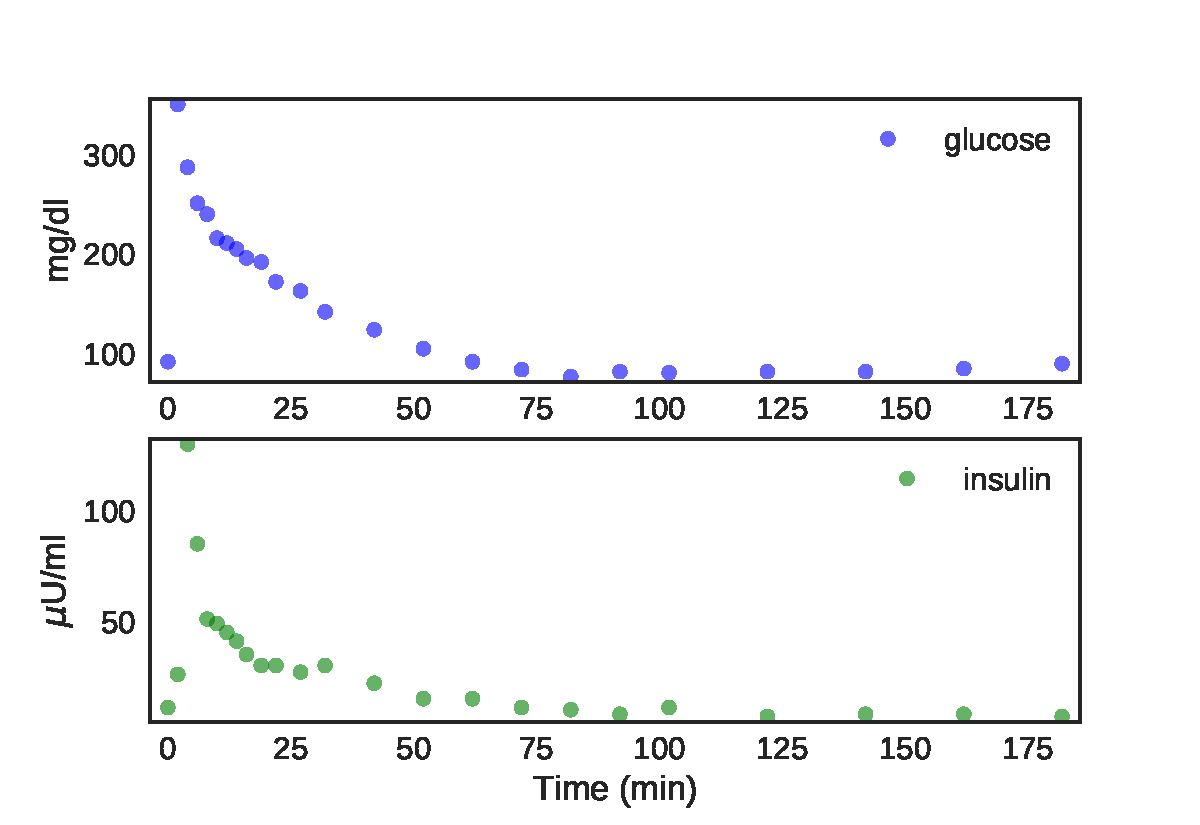
\includegraphics[height=3in]{figs/chap08-fig01.pdf}}
\caption{Glucose and insulin concentrations measured by IVGTT.}
\label{chap08-fig01}
\end{figure}

Figure~\ref{chap08-fig01} shows glucose and insulin concentrations over \SI{182}{\minute} for a subject with normal insulin production and sensitivity.

%TODO: consider siunitx settings for \per (as a fraction or negative power).



\section{Interpolation}

Before we are ready to implement the model, there's one problem we have to solve.  In the differential equations, $I$ is a function that can be evaluated at any time, $t$.  But in the \py{DataFrame}, we only have measurements at discreet times.  This is a job for interpolation!

\py{modsim.py} provides a function named \py{interpolate}, which is a wrapper for \py{scipy.interpolate.interp1d}.  It takes any kind of \py{Series} as a parameter, including \py{TimeSeries} and \py{Sweep}, and returns a function.  That's right, I said it returns a {\em function}.

So we can call it like this:

\begin{python}
I = interpolate(df.insulin)
\end{python}

And now we can call the new function, \py{I}, like this:

\begin{python}
I(18)
\end{python}

The result is 31.66, which is a linear interpolation between the actual measurements at \py{t=16} and \py{t=19}.  We can also run \py{I} with an array:

\begin{python}
ts = arange(0, 182, 2)
I(ts)
\end{python}

The result is an array of interpolated values for equally-spaced values of \py{t} between 0 and 182.

\py{interpolate} can take additional options as parameters, which it passed along to \py{scipy.interpolate.interp1d}.  You can read about these options at \url{https://docs.scipy.org/doc/scipy/reference/generated/scipy.interpolate.interp1d.html}.



\section{Implementing the model}
\section{glucose}

To get started, we'll assume that the parameters of the model are known.  We'll implement the model and use it to generate time series for \py{G} and \py{X}.  Then we'll see how to find parameter values that generate series that best fit the data.

Taking advantage of estimates from prior work, I'll start with these values:

\begin{python}
k1 = 0.03
k2 = 0.02
k3 = 1e-05
G0 = 290
\end{python}

And I'll use the measurements at \py{t=0} as the basal levels:

\begin{python}
Gb = df.glucose[0]
Ib = df.insulin[0]
\end{python}

Now we can create the initial state:

\begin{python}
init = State(G=G0, X=0)
\end{python}

And the \py{System} object:

\begin{python}
system = System(init=init, 
                k1=k1, k2=k2, k3=k3,
                I=I, Gb=Gb, Ib=Ib,
                t0=0, t_end=182, dt=2)
\end{python}

%TODO: Consider making System take a string argument like
%      System('init k1 k2 k3...')

Now here's the update function:

\begin{python}
def update_func(state, t, system):
    G, X = state
    unpack(system)
        
    dGdt = -k1 * (G - Gb) - X*G
    dXdt = k3 * (I(t) - Ib) - k2 * X
    
    G += dGdt * dt
    X += dXdt * dt

    return State(G=G, X=X)
\end{python}

As usual, the parameters include a \py{State} object with the current state and a \py{System} object with the system parameters.  But there's  one difference from previous examples: this update function also takes \py{t} as a parameter, because this system of differential equations is {\bf time-dependent}; that is, time appears in the right-hand side of at least one equation.  Specifically, we have to evaluate \py{I} at \py{t}.  

The first line uses multiple assignment to extract the current values of \py{G} and \py{X}.  The second line uses \py{unpack} to make the system variables available as if they were global variables, as we saw in Section~\ref{xxx}.  %TODO: add that section

Computing the derivatives \py{dGdt} and \py{dXdt} is straightforward; we just have to translate the equations from math notation to Python.

Then, to perform the update, we multiply each derivative by the discrete time step \py{dt}, which is \SI{2}{\minute} in this example.  The return value is a \py{State} object with the new values of \py{G} and \py{X}.

Before running the simulation, it is always a good idea to run the update function with the initial conditions:

\begin{python}
update_func(init, 0, system)
\end{python}

If there are no errors, and the results seem reasonable, we are ready to run the simulation.  Here's one more version of \py{run_simulation}.  It is almost the same as in Section~\ref{xxx}, with one change: it passes \py{t} as a parameter to \py{update_func}.

%TODO: Make this version consistent with Chapter 7

\begin{python}
def run_simulation(system, update_func):
    unpack(system)
    
    df = TimeFrame(columns=init.index)
    df.loc[t0] = init
    
    for t in arange(t0, t_end, dt):
        df.loc[t+dt] = update_func(df.loc[t], t, system)
    
    system.results = df
\end{python}

And we can run it like this:

\begin{python}
run_simulation(system, update_func)
\end{python}

\begin{figure}
\centerline{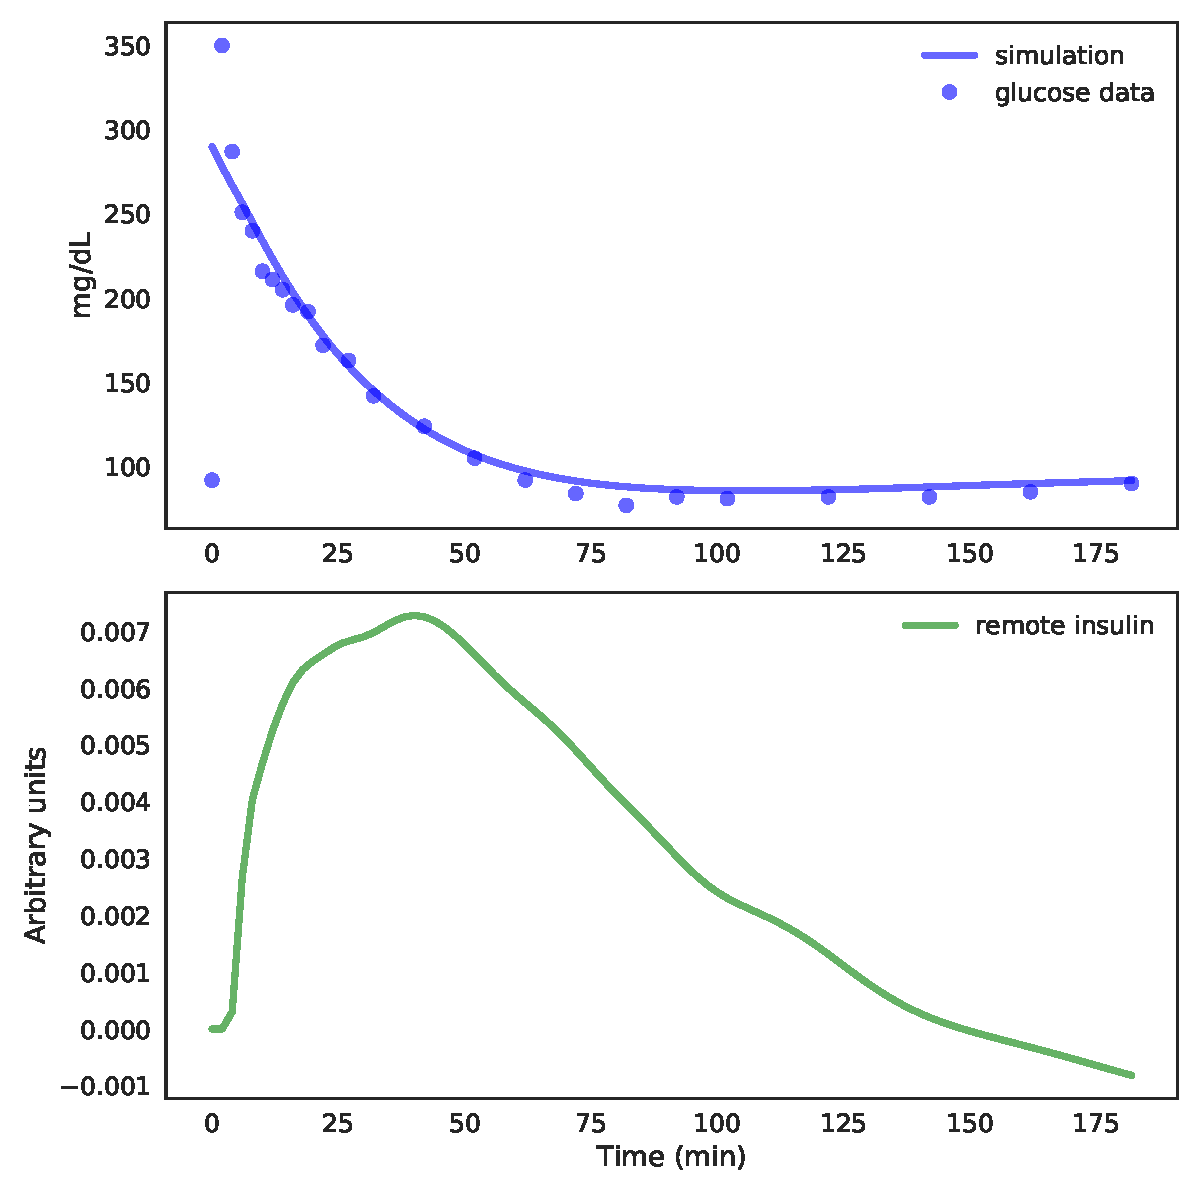
\includegraphics[height=3in]{figs/chap08-fig03.pdf}}
\caption{Results from simulation of the glucose minimal model.}
\label{chap08-fig03}
\end{figure}

The results are shown in Figure~\ref{chap08-fig03}.  The top plot shows simulated glucose levels from the model along with the measured data.  The bottom plot shows simulated insulin levels in tissue fluid, which is in unspecified units, and not to be confused with measured concentration of insulin in the blood.

With the parameters I chose, the model fits the data reasonably well.  We can do better, but first, I want to replace \py{run_simulation} with a better differential equation solver.


\section{Numerical solution of differential equations}
\label{slopefunc}

So far we have been solving differential equations by rewriting them as difference equations.  In the current example, the differential equations are:
%
\[ \frac{dG}{dt} = -k_1 \left[ G(t) - G_b \right] - X(t) G(t)  \]
%
\[ \frac{dX}{dt} = k_3 \left[I(t) - I_b \right] - k_2 X(t) \]
%
If we multiply both sides by $dt$, we have:
%
\[ dG = dt \left[ -k_1 \left[ G(t) - G_b \right] - X(t) G(t) \right] \]
%
\[ dX = dt \left[ k_3 \left[I(t) - I_b \right] - k_2 X(t) \right] \]
%
When $dt$ is very small, or more precisely infinitesimal, this equation is exact.  But in our simulations, $dt$ is \SI{2}{\minute}, which is small but not infinitesimal.  In effect, the simulations assume that the derivatives $dG/dt$ and $dX/dt$ are constant during each \SI{2}{\minute} time step.  That's not exactly true, but it can be a good enough approximation.

This method, evaluating derivatives at discrete time steps and assuming that they are constant in between, is called {\bf Euler's method} (see \url{https://en.wikipedia.org/wiki/Euler_method}).

Euler's method can be good enough for some simple problems, but there are many better ways to solve differential equations, including an entire family of methods called linear multistep methods (see \url{https://en.wikipedia.org/wiki/Linear_multistep_method}).

Rather than implement these methods ourselves, we will use functions from SciPy.  \py{modsim.py} provides a function called \py{run_odeint}, which is a wrapper for \py{scipy.integrate.odeint}.  The name \py{odeint} stands for ``ordinary differential equation integrator".  The equations we are solving are ``ordinary'' because all the derivatives are with respect to the same variable; in other words, there are no partial derivatives.  And the solver is called an integrator because solving differential equations is considered a form of integration.

\py{scipy.integrate.odeint} is a wrapper for \py{LSODA}, which is from ODEPACK, a venerable collection of ODE solvers written in Fortran (for some of the history of ODEPACK, see \url{http://history.siam.org/oralhistories/hindmarsh.htm}).

To use \py{odeint}, we have to provide a ``slope function":

\begin{python}
def slope_func(state, t, system):
    G, X = state
    unpack(system)
    
    dGdt = -k1 * (G - Gb) - X*G
    dXdt = k3 * (I(t) - Ib) - k2 * X
    
    return dGdt, dXdt
\end{python}

\py{slope_func} is similar to \py{update_func}; in fact, it takes the same parameters.  But \py{slope_func} is simpler, because all we have to do is compute the derivatives, that is, the slopes.  We don't have to do the updates; \py{odeint} does them for us.

Before we call \py{run_odeint}, we have to create a \py{System} object:

\begin{python}
system2 = System(init=init, 
                k1=k1, k2=k2, k3=k3,
                I=I, Gb=Gb, Ib=Ib,
                ts=df.index)
\end{python}

When we were using \py{run_simulation}, we created a \py{System} object with variables \py{t0}, \py{t_end}, and \py{dt}.  When we use \py{run_odeint}, we don't need those variables, but we do have to provide \py{ts}, which is an array or \py{Series} that contains the times where we want the solver to evaluate $G$ and $X$.

Now we can call \py{run_odeint} like this:

\begin{python}
run_odeint(system2, slope_func)
\end{python}

Like \py{run_simulation}, \py{run_odeint} puts the results in a \py{DataFrame} and stores it as a system variable named \py{results}.  The columns of \py{results} match the state variables in \py{init}.  The index of results match the values from \py{ts}; in this example, \py{ts} contains the timestamps of the measurements.

The results are similar to what we saw in Figure~\ref{chap08-fig03}.  The difference is about 1\% on average and never more than 2\%.


\section{Optimization}

So far we have been taking the parameters as given, but in general we don't have that luxury.  Normally we are given the data and we have to search for the parameters that yield a time series that best matches the data.

We will do that now, in two steps:

\begin{enumerate}

\item First we'll define an {\bf error function} that takes a set of possible parameters, simulates the system with the given parameters, and computes the difference between the simulation results and the data.

\item Then we'll use a library function from SciPy, \py{leastsq}, to search for the parameters that minimize the mean squared errors (MSE).

\end{enumerate}

Here's an outline of the functions we'll use:

\begin{itemize}

\item \py{modsim.py} provides \py{fit_leastsq}, which takes a function called \py{error_func} as a parameter.  It does some error-checking, then calls \py{scipy.optimize.leastsq}, which does the real work.

\item \py{scipy.optimize.leastsq} uses functions called \py{lmdif} and \py{lmdir}, which implement the Levenberg-Marquardt algorithm for non-linear least squares problems (see \url{https://en.wikipedia.org/wiki/Levenberg-Marquardt_algorithm}).  These functions are provided by another venerable FORTRAN library called MINPACK (see \url{https://en.wikipedia.org/wiki/MINPACK}).

\item When \py{scipy.optimize.leastsq} runs, it calls \py{error_func} many times, each time with a different set of parameters, until it converges on the set of parameters that minimizes MSE.

\end{itemize}

Each time the error function runs, it creates a \py{System} object with the given parameters, so let's wrap that operation in a function:

\begin{python}
def make_system(G0, k1, k2, k3, data):
    init = State(G=G0, X=0)
    system = System(init=init, 
                    k1=k1, k2=k2, k3=k3,
                    Gb=Gb, Ib=Ib, 
                    I=interpolate(data.insulin),
                    ts=data.index)
    return system
\end{python}

\py{make_system} takes \py{G0} and the rate constants as parameters, as well as \py{data}, which is the \py{DataFrame} containing the measurements.  It creates and returns a \py{System} object.

Now here's the error function:

\begin{python}
def error_func(params, data):
    system = make_system(*params, data)
    run_odeint(system, slope_func)
    error = system.results.G - data.glucose
    return error
\end{python}

The parameters of \py{error_func} are

\begin{itemize}

\item \py{params}, which is a sequence of four system parameters, and

\item \py{data}, which is the \py{DataFrame} containing the measurements.

\end{itemize}

It uses \py{make_system} to create the \py{System} object.  This line demonstrates a feature we have not seen before, the {\bf scatter operator}, \py{*}.  Applied to \py{params}, the scatter operator unpacks the sequence, so instead of being considered a single value, it is treated as four separate values.

\py{error_func} calls \py{run_odeint} using the same slope function we saw in Section~\ref{slopefunc}.  Then it computes the difference between the simulation results and the data.  Since \py{system.results.G} and \py{data.glucose} are both \py{Series} objects, the result of subtraction is also a \py{Series}.

Now to do the actual minimization, we run \py{fit_leastsq}:

\begin{python}
k1 = 0.03
k2 = 0.02
k3 = 1e-05
G0 = 290
params = G0, k1, k2, k3
best_params = fit_leastsq(error_func, params, df)
\end{python}

\py{error_func} is the function we just defined.  \py{params} is a sequence containing an initial guess for the four system parameters.  And \py{df} is the \py{DataFrame} containing the measurements.

Actually, the third parameter can be any object we like.  \py{fit_leastsq} and \py{leastsq} don't do anything with this parameter except to pass it along to \py{error_func}, so in general it contains whatever information \py{error_func} needs to do its job.


\section{Interpreting parameters}

The return value from \py{fit_leastsq} is \py{best_params}, which we can pass along to \py{make_system}, again using the scatter operator, and then run the simulation:

\begin{python}
system = make_system(*best_params, df)
run_odeint(system, slope_func)
\end{python}


\begin{figure}
\centerline{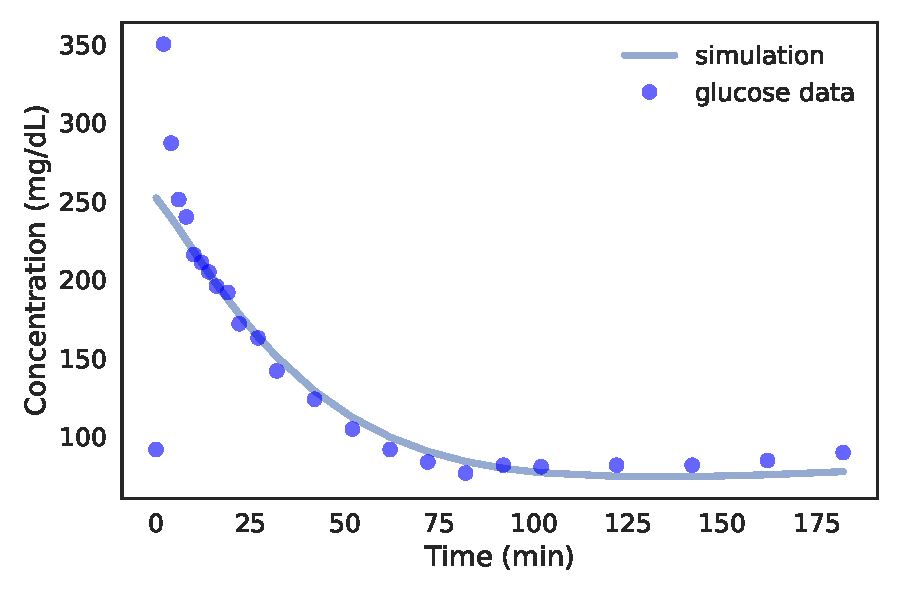
\includegraphics[height=3in]{figs/chap08-fig04.pdf}}
\caption{Simulation of the glucose minimal model with parameters that minimize MSE.}
\label{chap08-fig04}
\end{figure}

Figure~\ref{chap08-fig04} shows the results.  The simulation matches the measurements well, except during the first few minutes after the injection.  But we don't expect the model to do well in this regime.

The reason is that the model is {\bf non-spatial}; that is, it does not take into account differences in concentrations in different places in the body.  Instead, it assumes that the concentration of glucose and insulin in blood, and insulin in tissue fluid, is the same throughout the body.

Immediately after injection, it takes time for the injected glucose to circulate.  During that time, we don't expect a non-spatial model to be accurate.  For this reason, we should not take the estimated value of \py{G0} too seriously; it is useful for fitting the model, but not meant to correspond to a physical, measurable quantity.

On the other hand, the other parameters are meaningful; in fact, they are the reason the model is useful.  Using the best-fit parameters, we can estimate two quantities of interest:

\begin{itemize}

\item ``Glucose effectiveness", which is the tendency of elevated glucose to cause depletion of glucose.  

\item ``Insulin sensitivity", which is the ability of elevated blood insulin to enhance glucose effectiveness.

\end{itemize}

We can use the differential equations to compute these quantities.
%
\[ \frac{dG}{dt} = -k_1 \left[ G(t) - G_b \right] - X(t) G(t) \]
%
\[ \frac{dX}{dt} = k_3 \left[I(t) - I_b \right] - k_2 X(t) \]
%
Glucose effectiveness is defined as the change in $dG/dt$ as we vary $G$:
%
\[ E \equiv - \frac{\delta \dot{G}}{\delta G} \]
%
where $\dot{G}$ is shorthand for $dG/dt$.  Taking the derivative of $dG/dt$ with respect to $G$, we get
%
\[ E = k_1 + X \]
%
The glucose effectiveness index, $S_G$, is defined to be the value of $E$ in when blood insulin is near its basal level, $I_b$.  In that case, $X$ approaches 0 and $E$ approaches $k_1$.  So we can use the best-fit value of $k_1$ as an estimate of $S_G$.

The insulin sensitivity index, $S_I$, is defined to be the value of $S$ when $E$ and $I$ are at steady state:
%
\[ S_I \equiv \frac{\delta E_{SS}}{\delta I_{SS}} \]
%
$E$ and $I$ are at steady state when $dG/dt$ and $dX/dt$ are 0, but we don't actually have to solve those equations to find $S_I$.

If we set $dX/dt = 0$ and solve for $X$, we find the relation:
%
\[ X_{SS} = \frac{k_3}{k_2} I_{SS} \]
%
And since $E = k_1 + X$, we have:  
%
\[ S_I = \frac{\delta E_{SS}}{\delta I_{SS}} = \frac{\delta X_{SS}}{\delta I_{SS}} \]
%
Taking the derivative of $X_{SS}$ with respect to $I_{SS}$, we have:
%
\[ S_I = k3 / k2 \]
%
So if we find parameters that make the model fit the data, we can use $k_3 / k_2$ as an estimate of $S_I$.  

For the example data, the estimated values of $S_G$ and $S_I$ are $0.029$ and for $8.9 \times 10^{-4}$.  According to Pacini and Bergman, these values are within the normal range.


\section{The insulin minimal model}

In addition to the glucose minimal mode, Pacini and Bergman present an insulin minimal model, in which the concentration of insulin, $I$, is governed by this differential equation:
%
\[ \frac{dI}{dt} = -k I(t) + \gamma \left[ G(t) - G_T \right] t \]
%
where

\begin{itemize}

\item $k$ is a parameter that controls the rate of insulin disappearance independent of blood glucose.   

\item $G(t)$ is the measured concentration of blood glucose at time $t$.

\item $G_T$ is the glucose threshold; when blood glucose is above this level, it triggers an increase in blood insulin. 

\item $\gamma$ is a parameter that controls the rate of increase (or decrease) in blood insulin when glucose is above (or below) $G_T$.

% TODO: explain why t is there

\end{itemize}

The initial condition is $I(0) = I_0$.  As in the glucose minimal model, we treat the initial condition as a parameter which we'll choose to fit the data.

The parameters of this model can be used to estimate, $\phi_1$ and $\phi_2$, which are values that ``describe the sensitivity to glucose of the first and second phase pancreatic responsivity".  They are related to the parameters as follows:
%
\[ \phi_1 = \frac{I_{max} - I_b}{k (G_0 - G_b)}\]
%
\[ \phi_2 = \gamma \times 10^4 \]
%
where $I_{max}$ is the maximum measured insulin level, and $I_b$ and $G_b$ are the basal levels of insulin and glucose.

In the notebook for this chapter, you will have a chance to implement this model, find the parameters that best fit the data, and estimate these values.


\chapter{Projectiles}

So far the differential equations we've worked with have been {\bf first order}, which means they involve only first derivatives (see \url{https://en.wikipedia.org/wiki/Ordinary_differential_equation#General_definition}).  First order ODEs can be written
%
\[ \frac{dy}{dx} = F(x, y) \]
%
where $F$ is some function of $x$ and $y$.

In this chapter, we turn our attention to second order ODEs, which can involve both first and second derivatives.  Second order ODEs can be written
%
\[ \frac{d^2y}{dx^2} = G(x, y, y') \]
%
where $y'$ is shorthand for $dy/dx$.  In particular, we will work with one of the most famous, useful, and possibly the first second order ODE, Newton's second law of motion:
%
\[ F = m a \]
%
where $F$ is a force or the total of a set of forces, $m$ is the mass of a moving object, and $a$ is acceleration.

Newton's law might not look like a differential equation, until we realize that acceleration, $a$, is the second derivative of position, $y$, with respect to time, $t$.  With the substitution
%
\[ a = \frac{d^2y}{dt^2} \]
%
Newton's law can be written
%
\[ \frac{d^2y}{dt^2} = F / m \]
%
And that's definitely a second order ODE.  In general, $F$ can be a function of time, position, and velocity.  Mass is often constant, but can also depend on time, position, and velocity.

Of course, this ``law" is really a model, in the sense that it is a simplification of the real world.  Although it is often approximately true, it is not a good model for very small things, which are better described by another model, quantum mechanics.  And it is not a good model for things moving very fast, which are better described by relativistic mechanics.

But for things that are medium to large, moving at speeds that are medium to slow, Newton's model is a phenomenally useful.  In general, if we know what forces act on an object, we can figure out how it will move.

\section{Dropping pennies}

As a first example, let's get back to the penny falling from the Empire State Building, which we considered in Section~\ref{penny}.  We will implement two models of this system, first without air resistance, so the only force acting on the penny is gravity.  Then we'll add air resistance.

Given that the Empire State Building is \SI{381}{\meter} high, and assuming that the penny is dropped with 0 velocity, the initial conditions are:

\begin{python}
init = State(y=381 * m, 
             v=0 * m/s)
\end{python}

where \py{y} is height above the sidewalk and \py{v} is velocity.  The units \py{m} and \py{s} are from the \py{UNITS} object provided by Pint:

\begin{python}
m = UNITS.meter
s = UNITS.second
\end{python}

The only system parameter is the acceleration of gravity:

\begin{python}
g = 9.8 * m/s**2
\end{python}

In addition, we'll specify the sequence of times where we want to solve the differential equation:

\begin{python}
duration = 10 * s
ts = linspace(0, duration, 11)
\end{python}

\py{ts} contains 11 points between 0 and \SI{10}{\second}, including both endpoints.

%TODO: make linspace work with units?

Next we need a \py{System} object to contains the system parameters:

\begin{python}
system = System(init=init, g=g, ts=ts)
\end{python}

Now we need a slope function, and here's where things get tricky.  As we have seen, \py{odeint} can solve systems of first order ODEs, but Newton's law is a second order ODE.

However, if we recognize that

\begin{enumerate}

\item Velocity, $v$, is the derivative of position, $dy/dt$, and

\item Acceleration, $a$, is the derivative of velocity, $dv/dt$

\end{enumerate}

we can rewrite Newton's law as a system of first order ODEs:
%
\[ \frac{dy}{dt} = v \]
%
\[ \frac{dv}{dt} = a \]
%
And we can translate those equations into a slope function:

\begin{python}
def slope_func(state, t, system):
    y, v = state
    unpack(system)    

    dydt = v
    dvdt = -g
    
    return dydt, dvdt
\end{python}

The first parameter, \py{state}, contains the position and velocity of the penny.  The last parameter, \py{system}, contains the system parameter \py{g}, which is the magnitude of acceleration due to gravity.

The second parameter, \py{t}, is time.  It is not used in this slope function because none of the factors of the model are time-dependent (see Section~\ref{glucose}).  I include \py{t} as a parameter anyway because this function will be called by \py{odeint}, and \py{odeint} always provides the same arguments, whether they are needed or not.

The rest of the function is a straightforward translation of the differential equations, with the substitution $a = -g$, which indicates that acceleration is due to gravity, in the direction of decreasing $y$.

The return value is a sequence containing the two derivatives.

Before calling \py{odeint}, it is always a good idea to test the slope function with the initial conditions:

\begin{python}
slope_func(init, 0, system)
\end{python}

The result is a sequence containing \SI{0}{\meter\per\second} for velocity and \SI{-9.8}{\meter\per\second\squared} for acceleration.

Now we can run \py{odeint} like this:

\begin{python}
run_odeint(system, slope_func)
\end{python}

\py{run_odeint} stores the results in a \py{DataFrame} with two columns: \py{y} contains the height of the penny as a function of time; \py{v} contains velocity.  \py{plot_results}, which is defined in the notebook for this chapter, plots height versus time:

\begin{python}
plot_results(system.results)
\end{python}

\begin{figure}
\centerline{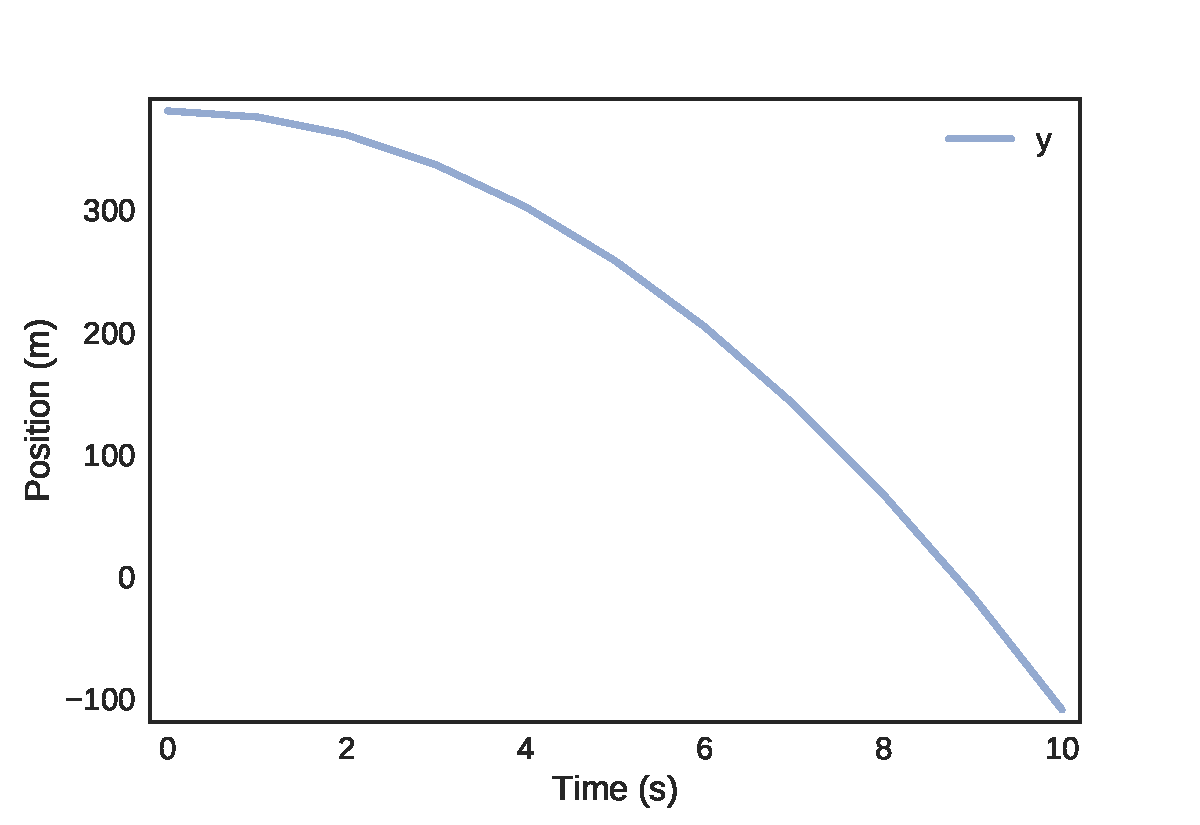
\includegraphics[height=3in]{figs/chap09-fig01.pdf}}
\caption{Height of the penny versus time, with no air resistance.}
\label{chap09-fig01}
\end{figure}

Figure~\ref{chap09-fig01} shows the result.  Since acceleration is constant, velocity increases linearly and position decreases quadratically; as a result, the height curve is a parabola.

In this model, height can be negative, because we have not included the effect of the sidewalk!


\section{Onto the sidewalk}

To avoid negative heights, we can use the results from the previous section to estimate when the penny hits the sidewalk, and run the simulation for the estimated time.

From the results, we can extract \py{y}, which is a \py{TimeSeries} that represents height as a function of time.

\begin{python}
y = system.results.y
\end{python}

But what we really want is the inverse function, time as a function of height, which we can represent by creating a \py{Series} object with the data and index from \py{y}, but reversed:

%TODO: check previous use of Series and see if we use `data` consistently
% instead of values

\begin{python}
inverse = Series(data=y.index, index=y.data)
\end{python}

Now we can use \py{interpolate}, which returns a function:

\begin{python}
T = interpolate(inverse, kind='cubic')
\end{python}

In this case I'm using a cubic spline, rather than linear interpolation, because it should do a better job of filling in the curve correctly (see \url{https://en.wikipedia.org/wiki/Spline_interpolation}).

Now we can evaluate the interpolating function at \py{y=0}

\begin{python}
T_sidewalk = T(0)
\end{python}

The result is \SI{8.8179}{\meter}, which agrees with the exact answer to 4 decimal places.

One caution about using \py{interpolate}: the function has to be single valued (see \url{https://en.wikipedia.org/wiki/Single-valued_function}.  In this example, height decreases monotonically, so for every height there is only one corresponding time.  But if we threw the penny upward and then it fell down, the penny would pass through some heights more than once.  In that case the inverse function represented by \py{T} would not be single valued, and \py{interpolate} would behave unpredictably.


\section{With air resistance}

As an object moves through fluid, including air, the object applies force to the air and, in accordance with Newton's third law of motion, the air applies an equal and opposite force to the object (see \url{https://en.wikipedia.org/wiki/Newton's_laws_of_motion}).

The direction of this {\bf drag force} is opposite the direction of travel, and its magnitude is given by the drag equation (see \url{https://en.wikipedia.org/wiki/Drag_equation}):
%
\[ F_d = \frac{1}{2}~\rho~v^2~C_d~A \]
%
where

\begin{itemize}

\item $F_d$ is force due to drag, in \si{\newton} (assuming as are using SI units).

\item $\rho$ is the density of the fluid in \si{\kg\per\meter\cubed}.

\item $v$ is velocity in \si{\meter\per\second}.

\item $A$ is the reference area of the object, in \si{\meter\squared}; in this context the reference area is the projected frontal area, that is, the visible area of the object as seen from a point on its line of travel (and far away).

\item $C_d$ is the {\bf drag coefficient}, a dimensionless quantity that depends on the shape of the object (including length but not frontal area), its surface properties, and how it interacts with the fluid.

\end{itemize}

For objects moving at moderate speeds through air, typical drag coefficients are between 0.1 and 1.0, with blunt objects at the high end and streamlined objects at the low end (see \url{https://en.wikipedia.org/wiki/Drag_coefficient}).

For simple geometric objects we can sometimes guess the drag coefficient with reasonable accuracy; for more complex objects we usually have to take measurements and estimate $C_d$ from the data.

Of course, the drag equation is itself a model, based on the primary assumption that $C_d$ does not depend on the other terms in the equation, density, velocity, and area.  For objects moving in air at moderate speeds (below 45 mph or \SI{20}{\meter\per\second}), this model might be good enough, but we should remember to revisit these assumptions.

%TODO: exercise with C_d(v)

For the falling penny, we can use measurements of falling pennies to estimate $C_d$.  According to Louis Bloomfield at the University of Virginia, the {\bf terminal velocity} of a penny is about 25 mph or \SI{11}{\meter\per\second} (see \url{https://www.scientificamerican.com/article/could-a-penny-dropped-off/}).

Terminal velocity is the speed where drag force equals force due to gravity:
%
\[ \frac{1}{2}~\rho~v_{term}^2~C_d~A = m g \]
%
where $m$ is the mass of the object and $g$ is acceleration due to gravity.  Solving this equation for $C_d$ yields:
%
\[ C_d = \frac{2~m g}{\rho~v_{term}^2~A} \]
%
According to Mythbusters, the terminal velocity of a penny is between 35 and 65 mph (see \url{https://en.wikipedia.org/wiki/MythBusters_(2003_season)}.  Using the low end of their range, 40 mph or about \SI{18}{\meter\per\second}, the estimated value of $C_d$ is 0.44, which is close to the drag coefficient of a smooth sphere.

Now we are ready to add air resistance to the model.


\section{Implementation}

As the number of system parameters increases, and as we need to do more work to compute them, we will find it useful to define a \py{Condition} object to contain the quantities we need to make a \py{System} object.

The way we create a \py{Condition} object is the same as for \py{System} and \py{State} object.  In fact, these three object type have the same capabilities; I have given them different names just to identify their different roles.  Here's the \py{Condition} object for the falling penny:

\begin{python}
condition = Condition(height = 381 * m,
                      g = 9.8 * m/s**2,
                      mass = 2.5e-3 * kg,
                      diameter = 19e-3 * m,
                      rho = 1.2 * kg/m**3,
                      v_term = 22 * m / s,
                      duration = 30)
\end{python}

The mass and diameter of a penny are from \url{https://en.wikipedia.org/wiki/Penny_(United_States_coin)}.  The density of air depends on temperature, barometric pressure (which depends on altitude), humidity, and composition (\url{https://en.wikipedia.org/wiki/Density_of_air}).  I chose a value that might be typical in New York City at \SI{20}{\celsius}.

And here's the function that takes a \py{Condition} as a parameter and returns a \py{System}:

\begin{python}
def make_system(condition):    
    unpack(condition)
    
    init = State(y=height, v=0 * m/s)
    area = np.pi * (diameter/2)**2
    C_d = 2 * mass * g / (rho * area * v_term**2)
    ts = linspace(0, duration, 101)
    
    return System(init=init, g=g, mass=mass, rho=rho,
                  c_d=c_d, area=area, ts=ts)
\end{python}

It might not be obvious why we need \py{Condition} objects.  One reason is to minimize the number of system parameters.  For example, we use \py{diameter} to compute \py{area} and \py{v_term} to compute \py{C_d}, but then we don't need \py{diameter} and \py{v_term} in the \py{System} object.

Another reason is that the \py{Condition} object will be useful, later in this chapter, because we can modify it, in a loop, to create a sequence of \py{System} objects, each with a different set of conditions.

For now, you might have to take my word that this is a good idea (see \url{https://zen-of-python.info/namespaces-are-one-honking-great-idea--lets-do-more-of-those.html}).

Now we can make a \py{System} like this:

\begin{python}
system = make_system(condition)
\end{python}

And write a version of the slope function that includes drag:

\begin{python}
def slope_func(state, t, system):
    y, v = state
    unpack(system)
    
    f_drag = rho * v**2 * C_d * area / 2
    a_drag = f_drag / mass
    
    dydt = v
    dvdt = -g + a_drag
    
    return dydt, dvdt
\end{python}

\py{f_drag} is the force due to drag, based on the drag equation.  \py{a_drag} is acceleration due to drag, based on Newton's second law.

To compute total acceleration, we add accelerations due to gravity and drag, where \py{g} is negated because it is in the direction of decreasing \py{y}, and \py{a_drag} is positive because it is in the direction of increasing \py{y}.  Soon we will see a way to keep track of the direction of forces and add them up in a less error-prone way.

After we test the slope function, we can run the simulation like this:

\begin{python}
run_odeint(system, slope_func)
\end{python}

\begin{figure}
\centerline{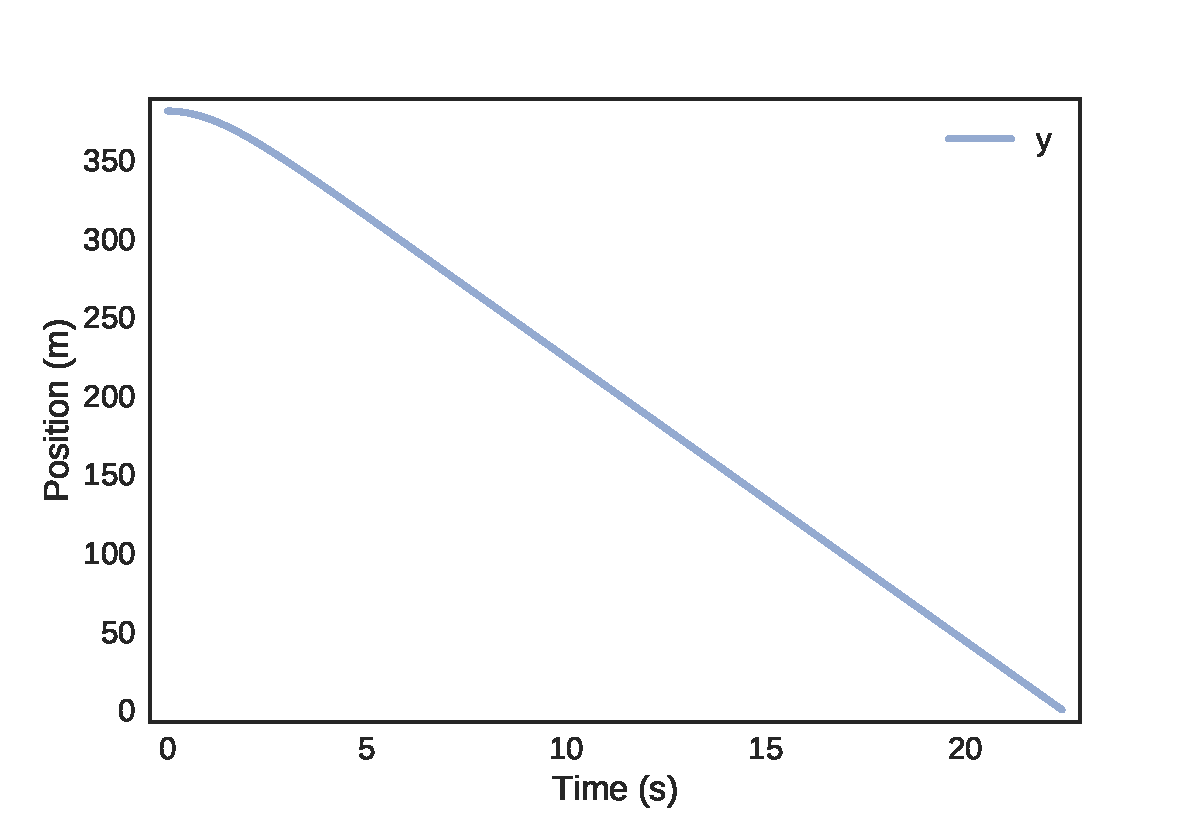
\includegraphics[height=3in]{figs/chap09-fig02.pdf}}
\caption{Height of the penny versus time, with air resistance.}
\label{chap09-fig02}
\end{figure}

Figure~\ref{chap09-fig02} shows the result.  It only takes a few second for the penny to accelerate up to terminal velocity; after that, velocity is constant, so height as a function of time is a straight line.

Now let's move on to two dimensions, and baseball!


\section{The Manny Ramirez problem}

Manny Ramirez is a former member of the Boston Red Sox who was notorious for a work ethic his managers did not always appreciate, which is why is he a former member.  The objective of this problem is to solve the following Manny-inspired problem:

{\it What is the minimum effort required to hit a home run in Fenway Park?}

We'll proceed in the following steps:

\begin{enumerate}

\item

\item

\item

\end{enumerate}


The Green Monster in Fenway Park is about \SI{12}{\meter} high and about \SI{97}{\meter} from home plate along the left field line.  What is the minimum speed a ball must leave the bat in order to clear the monster (assuming it goes off at the optimal angle, for some definition of "optimal")?




\backmatter
\printindex

\end{document}

\end{itemize}
